\documentclass{article}

\title{
	Using Constraints to Discover Sparse and Alternative Subgroup Descriptions
}
\author{
	Jakob Bach~\orcidlink{0000-0003-0301-2798}\\
	\small Karlsruhe Institute of Technology (KIT), Germany\\
	\small \href{mailto:jakob.bach@kit.edu}{jakob.bach@kit.edu}
}
\date{} % don't display a date

\usepackage[style=numeric, backend=bibtex]{biblatex}
\usepackage[ruled,linesnumbered,vlined]{algorithm2e} % pseudo-code
\usepackage{amsmath} % mathematical symbols
\usepackage{amssymb} % mathematical symbols
\usepackage{amsthm} % theorems, definitions etc.
\usepackage{booktabs} % nicely formatted tables (with top, mid, and bottom rule)
\usepackage{enumitem} % customized enumerations
\usepackage{graphicx} % plots
\usepackage{multirow} % cells spanning multiple rows in tables
\usepackage{orcidlink} % ORCID icon
\usepackage{subcaption} % figures with multiple sub-figures and sub-captions
\usepackage{hyperref} % links and URLs

\addbibresource{references.bib}

\newtheorem{proposition}{Proposition}
\theoremstyle{definition}
\newtheorem{definition}{Definition}

\begin{document}

\maketitle

\begin{abstract}
Subgroup-discovery methods allow users to obtain simple descriptions of interesting regions in a dataset.
Using constraints in subgroup discovery can enhance interpretability even further.
In this article, we focus on two types of constraints:
First, we limit the number of features used in subgroup descriptions, making the latter sparse.
Second, we propose the novel optimization problem of finding alternative subgroup descriptions, which cover similar data objects as a given subgroup but use different features.
For both constraint types, we describe how to integrate them into heuristic search methods for subgroups.
Further, we propose a novel Satisfiability Module Theories (SMT) formulation of subgroup discovery as a white-box optimization problem, which allows solver-based search and is open for a variety of constraint types.
Additionally, we prove that both constraint types lead to an $\mathcal{NP}$-hard optimization problem.
Finally, we employ 27 binary-classification datasets to compare heuristic and solver-based search for unconstrained and constrained subgroup discovery.
We observe that heuristic search methods often yield subgroups of high quality within a short runtime, also in scenarios with constraints.
\end{abstract}
%
\textbf{Keywords:} subgroup discovery, alternatives, constraints, satisfiability modulo theories, explainability, interpretability, XAI

\section{Introduction}
\label{sec:csd:introduction}

\paragraph{Motivation}

The interpretability of prediction models has significantly gained importance in recent years~\cite{carvalho2019machine, molnar2020interpretable}.
There are various ways to foster interpretability in machine-learning pipelines.
In particular, some machine-learning models are simple enough to be intrinsically interpretable~\cite{carvalho2019machine}.
Subgroup-discovery methods fall into this category~\cite{atzmueller2015subgroup}.
The goal of subgroup discovery is to find `interesting' subgroups, i.e., subsets of a dataset, e.g., data objects where the prediction target takes a particular value.
Further, such subgroups should be described with a combination of simple conditions on feature values.
E.g., Figure~\ref{fig:csd:exemplary-subgroup} displays a rectangle-shaped subgroup description for a two-dimensional, real-valued dataset with a binary prediction target.
This subgroup is defined by $(\mathit{Feature\_1} \in [3.0, 5.1]) \land (\mathit{Feature\_2} \in [1.0, 1.8])$ and contains a considerably higher fraction of data objects with $\mathit{Target} = 1$ than the complete dataset.
While such subgroup descriptions already tend to be understandable for users, we see further potential to increase interpretability with the help of constraints.

\begin{figure}[t]
	\centering
	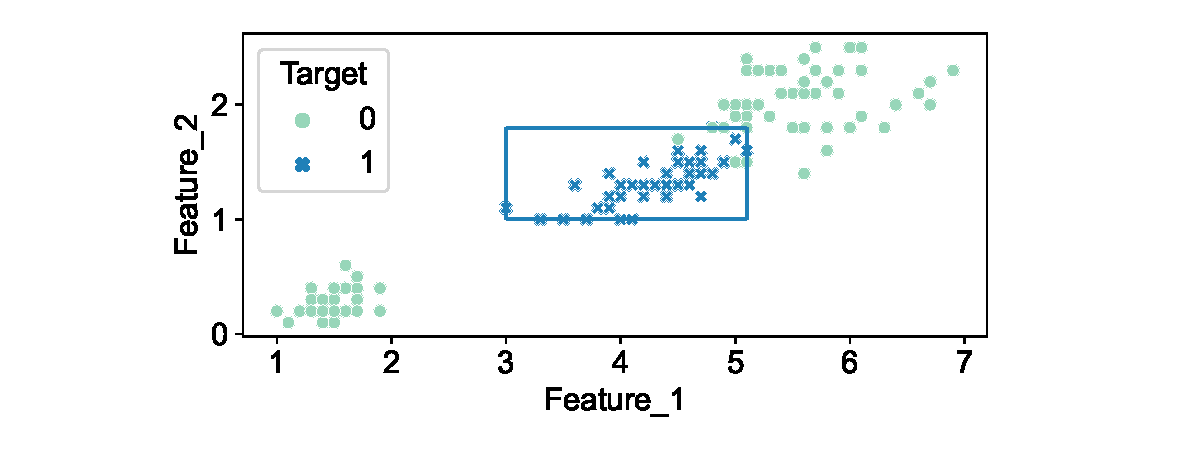
\includegraphics[width=\textwidth, trim=15 20 15 15, clip]{plots/csd-exemplary-subgroup.pdf}
	\caption{
		Exemplary subgroup description in the form a rectangle for a dataset with two real-valued features and a binary prediction target.
	}
	\label{fig:csd:exemplary-subgroup}
\end{figure}

\paragraph{Problem statement}

This article addresses the problem of constrained subgroup discovery.
In particular, we focus on two types of constraints related to the features used in subgroup descriptions:

First, \emph{feature-cardinality constraints} limit the number of selected features, i.e., features used in subgroup descriptions.
E.g., in Figure~\ref{fig:csd:exemplary-subgroup}, one may use only either feature to define a subgroup with $\mathit{Target} = 1$ instead of using both features, thereby simplifying the subgroup description but inevitably capturing more data objects with $\mathit{Target} = 0$.
With feature selection, the subgroup descriptions become \emph{sparse}, which increases their interpretability.
In particular, even intrinsically interpretable model may loose interpretability if they involve too many features~\cite{molnar2020interpretable}.
This constraint type resembles feature selection~\cite{guyon2003introduction, li2017feature}, which is a common task in machine-learning pipelines.

Second, we formulate constraints to search \emph{alternative subgroup descriptions}:
Given an \emph{original} subgroup, an alternative subgroup should reproduce the set of contained data objects as closely as possible but use different features in its subgroup description.
E.g., in Figure~\ref{fig:csd:exemplary-subgroup}, one may define a subgroup with an interval one feature and then try to capture a similar set of data objects with the other feature.
With alternative subgroup descriptions, users obtain different explanations for the same subgroup.
Such alternative explanations are also popular in other explainable-AI techniques like counterfactuals~\cite{mothilal2020explaining, russell2019efficient}, e.g., to enable users to develop and test multiple hypotheses or foster trust in the predictions~\cite{kim2021multi, wang2019designing}.

\paragraph{Related work}

There are various search methods for subgroup discovery, exact~\cite{atzmueller2006sd, bosc2018anytime, grosskreutz2009subgroup, lemmerich2010fast} as well as heuristic~\cite{friedman1999bump, leeuwen2012diverse, mampaey2012efficient, proencca2022robust} ones.
We see research gaps in three aspects:
First, all widely used subgroup-discovery methods are algorithmic in nature and only support a limited set of constraints, as the search routines need to be specifically adapted to particular constraint types.
Second, the number of features used in a subgroup description is a well-known measure for subgroup complexity~\cite{helal2016subgroup, herrera2011overview, ventura2018subgroup}.
However, there is a lack of systematic evaluations of this constraint type, particularly evaluations with different cardinality thresholds and comparing multiple subgroup-discovery methods.
Third, various subgroup-discovery methods yield a diverse set of subgroups rather than only one subgroup, thereby providing alternative solutions~\cite{belfodil2019fssd, bosc2018anytime, leeuwen2012diverse, lemmerich2010fast, lucas2018ssdp+, proencca2022robust}.
However, this notion of alternatives targets at capturing different subsets of data objects from the dataset.
In contrast, our notion of alternative subgroup descriptions tries to capture the same data objects as in the original subgroup but with different features in the description.

\paragraph{Contributions}

Our contribution is fivefold:

First, we formalize subgroup discovery as a Satisfiability Modulo Theories (SMT) optimization problem.
This novel white-box formulation admits solver-based search for subgroups and allows integrating a broad range of constraints.

Second, we formalize two constraint types for this optimization problem, i.e., feature-cardinality constraints and alternative subgroup descriptions.
For the latter, we allow users to control alternatives with two parameters, i.e., the number of alternatives and a dissimilarity threshold.
We integrate both constraint types into our white-box formulation of subgroup discovery.

Third, we describe how to integrate these two constraint types into three existing heuristic search methods and two novel baselines for subgroup discovery.
The latter are faster and simpler than the former, so they may serve as additional reference points for future experimental studies on subgroup discovery.

Fourth, we analyze the computational complexity of the subgroup-discovery problem with each of these two constraint types.
In particular, prove several $\mathcal{NP}$-hardness results and thereby show that finding optimal solutions under these constraint types is not trivial.

Fifth, we conduct comprehensive experiments with 27 binary-classification datasets from the Penn Machine Learning Benchmarks (PMLB)~\cite{olson2017pmlb, romano2021pmlb}.
We evaluate the runtime of subgroup discovery and the quality of the discovered subgroups.
In particular, we compare solver-based and heuristic subgroup-discovery methods without constraints, with a feature-cardinality constraint, and for searching alternative subgroup descriptions.
We also analyze how the subgroup quality in solver-based search depends on the timeout of the solver.
We publish all code\footnote{\url{https://github.com/Jakob-Bach/Constrained-Subgroup-Discovery}} and experimental data\footnote{TODO} online.

\paragraph{Experimental results}

In our experimental scenario without constraints, the heuristic search methods yield similar subgroup quality as solver-based search.
On the test set, the heuristics may even be better since they show less overfitting, i.e., a lower gap between training-set quality and test-set quality.
Additionally, the solver-based search is considerably slower.
Using a solver timeout, a large fraction of the final subgroup quality can be reached in a fraction of the runtime, though this quality is lower than for equally fast heuristics.

With a feature-cardinality constraint, heuristic search methods still are competitive quality-wise compared to solver-based search.
Further, subgroups only using a few features show relatively high quality compared to unconstrained subgroups.
I.e., there is a decreasing marginal utility in selecting more features.
Additionally, feature-cardinality constraints reduce overfitting.

For alternative subgroup description, heuristics also yield similar quality as solver-based search.
Our two user parameters for alternatives control the solutions as expected:
The similarity to the original subgroup and the quality of the alternatives decrease for more alternatives and a higher dissimilarity threshold.

\paragraph{Outline}

Section~\ref{sec:csd:fundamentals} introduces fundamentals.
Section~\ref{sec:csd:baselines} proposes two baselines for subgroup discovery.
Section~\ref{sec:csd:approach} describes and analyzes constrained subgroup discovery.
Section~\ref{sec:csd:experimental-design} outlines our experimental design, while Section~\ref{sec:csd:evaluation} presents the experimental results.
Section~\ref{sec:csd:related-work} reviews related work.
Section~\ref{sec:csd:conclusion} concludes and discusses future work.
Appendix~\ref{sec:csd:appendix} contains supplementary materials.

\section{Fundamentals of Subgroup Discovery}
\label{sec:csd:fundamentals}

In this section, we describe fundamentals for our work.
First, we introduce the optimization problem of subgroup discovery (cf.~Section~\ref{sec:csd:fundamentals:problem}).
Second, we describe common heuristic search methods to solve this problem (cf.~Section~\ref{sec:csd:fundamentals:heuristics}).

\subsection{Problem}
\label{sec:csd:fundamentals:problem}

\paragraph{Context}

In general, subgroup discovery involves finding descriptions of interesting subsets of a dataset~\cite{atzmueller2015subgroup}.
There are multiple options to define the type of dataset, the kind of subgroup description, and the criterion of interestingness.
In the following, we formalize the notion of subgroup discovery that we tackle in this article.
For broader surveys, see~\cite{atzmueller2015subgroup, helal2016subgroup, herrera2011overview, ventura2018subgroup}.

\paragraph{Dataset}

We focus on tabular, real-valued data.
In particular, $X \in \mathbb{R}^{m \times n}$ stands for a dataset in the form of a matrix.
Each row is a data object, and each column is a feature.
We assume that categorical features have already been made numeric, e.g., via one-hot or ordinal encoding.
There are also many subgroup-discovery methods that only process categorical data and require continuous features to be discretized~\cite{herrera2011overview, meeng2021real}.
$X_{i \cdot} \in \mathbb{R}^n$ denotes the values of all features for the $i$-th data object,
while $X_{\cdot j} \in \mathbb{R}^m$ denotes the values of the $j$-th feature for all data objects.
$y \in Y^m$ represents the prediction target with domain $Y$, e.g., $Y=\{0,1\}$ for binary classification or $Y=\mathbb{R}$ for regression.
Thus, we are in a supervised-learning scenario.
In this article, we focus on binary-classification scenarios in our formalization and evaluation.
In general, one may also conduct subgroup discovery in multi-class, multi-target, or regression scenarios~\cite{atzmueller2015subgroup}.

\paragraph{Subgroup}

A Subgroup description typically comprises a conjunction of conditions on individual features~\cite{meeng2021real}.
For real-valued data, the conditions constitute intervals.
Thus, a subgroup description is a hyperrectangle.
In particular, the subgroup description comprises a lower bound and an upper bound for each feature.
The bounds for a feature may also be infinite to leave it unrestricted.
A data object resides in the subgroup if all its feature values are in the intervals formed by lower and upper bounds:
%
\begin{definition}[Subgroup (description)]
	Given a dataset~$X \in \mathbb{R}^{m \times n}$, a \emph{subgroup} is described by its lower bounds~$\mathit{lb} \in \{\mathbb{R} \cup \{-\infty, +\infty\}\}^n$ and upper bounds~$\mathit{ub} \in \{\mathbb{R} \cup \{-\infty, +\infty\}\}^n$.
	Data object $X_{i \cdot}$ is a \emph{member} of this subgroup if $\forall j \in \{1, \dots, n\}:~ \left( X_{ij} \geq \mathit{lb}_j \right) \land \left( X_{ij} \leq \mathit{ub}_j \right)$.
	\label{def:csd:subgroup}
\end{definition}
%
For categorical features, one may replace the inequality comparisons with equality comparisons against categorical feature values~\cite{atzmueller2015subgroup}.

Throughout this article, we often use the terms \emph{subgroup} and \emph{subgroup description} interchangeably.
In a more strict sense, one may use the former term to denote the subgroup's members and the latter for the subgroup's bounds~\cite{atzmueller2015subgroup}.

\paragraph{Subgroup discovery}

For framing subgroup discovery as an optimization problem, we need a notion of subgroup quality, i.e., interestingness of the subgroup.
A function $Q(\mathit{lb}, \mathit{ub}, X, y)$ shall return the quality of a subgroup on a particular dataset.
Without loss of generality, we assume that this function should be maximized:
%
\begin{definition}[Subgroup discovery]
	Given a dataset~$X \in \mathbb{R}^{m \times n}$ with prediction target~$y \in \{0, 1\}^m$,
	\emph{subgroup discovery} is the problem of finding a subgroup (cf.~Definition~\ref{def:csd:subgroup}) with bounds~$\mathit{lb}, \mathit{ub} \in \{\mathbb{R} \cup \{-\infty, +\infty\}\}^n$ that maximizes a given notion of subgroup quality~$Q(\mathit{lb}, \mathit{ub}, X, y)$.
	\label{def:csd:subgroup-discovery}
\end{definition}
%
While this definition refers to one subgroup, some subgroup-discovery methods may also return a set of subgroups~\cite{atzmueller2015subgroup}.

For binary-classification scenarios, interesting subgroups should typically contain many data objects from one class but few from the other class.
While traditional classification tries to characterize the dataset globally, subgroup discovery follows a local paradigm, i.e., focuses on the data objects in the subgroup~\cite{meeng2021real}.
Without loss of generality, we assume that the class with label~`1' is the class of interest, also called \emph{positive} class.

\paragraph{Subgroup quality}

Weighted Relative Accuracy (WRAcc)~\cite{lavravc1999rule} is a popular metric for subgroup quality~\cite{meeng2021real}:
%
\begin{equation}
	\text{WRACC} = \frac{m_b}{m} \cdot \left( \frac{m_b^+}{m_b} - \frac{m^+}{m} \right)
	\label{eq:csd:wracc}
\end{equation}
%
Besides the total number of data objects~$m$, this metric considers the number of positive data objects~$m^+$, the number of data objects in the subgroup~$m_b$, and the number of positive data objects in the subgroup~$m_b^+$.
In particular, WRAcc is the product of two factors:
$m_b / m$ quantifies the generality of the subgroup with the relative frequency of subgroup membership.
The second factor measures the difference in relative frequency of the positive class between the subgroup and the whole dataset, i.e., the relative accuracy of the subgroup.
If the subgroup contains the same fraction of positive data objects as the whole dataset, WRAcc is zero.
The theoretical maximum and minimum of WRAcc depend on the class frequencies in the dataset.
In particular, the maximum WRAcc for a dataset equals the product of the relative frequencies of positive and negative data objects in the dataset:
%
\begin{equation}
	\text{WRACC}_{\text{max}} = \frac{m^+}{m} \cdot \left( 1 - \frac{m^+}{m} \right)
	\label{eq:csd:wracc-max}
\end{equation}
%
This maximum is reached if all positive data objects are in the subgroup and all negative data objects are outside, i.e., $m_b^+ = m_b = m^+$.
Depending on the feature values of the dataset, a corresponding subgroup description may not exist.
Further, while the maximum is 0.25 if both classes occur with equal frequency, it becomes smaller the more imbalanced the classes are.
Thus, it makes sense to normalize WRAcc when working with datasets with different class frequencies.
One normalization, which we use in our experiments, is a max-normalization to the range $[-1, 1]$~\cite{mathonat2021anytime}:
%
\begin{equation}
	\text{nWRACC} = \frac{\text{WRACC}}{\text{WRACC}_{\text{max}}} = \frac{m_b^+ \cdot m - m^+ \cdot m_b}{m^+ \cdot (m - m^+)}
	\label{eq:csd:wracc-normalized}
\end{equation}
%
Alternatively, one can also min-max normalize the range to~$[0, 1]$~\cite{carmona2018unifying, ventura2018subgroup}.

\subsection{Heuristic Search Methods}
\label{sec:csd:fundamentals:heuristics}

In general, there are heuristic and exhaustive search methods for subgroup discovery~\cite{atzmueller2015subgroup}.
In this section, we discuss three heuristic search methods, which we will employ in our experiments.
All three methods are well-established and originate from related work.

\begin{algorithm}[p]
	\DontPrintSemicolon
	\KwIn{Dataset~$X \in \mathbb{R}^{m \times n}$, \newline
		Prediction target~$y \in \{0, 1\}^m$, \newline
		Subgroup-quality function~$Q(\mathit{lb}, \mathit{ub}, X, y)$, \newline
		Peeling fraction~$\alpha \in (0, 1)$, \newline
		Support threshold~$\beta_0 \in [0, 1]$
	}
	\KwOut{Subgroup bounds~$\mathit{lb}, \mathit{ub} \in \{\mathbb{R} \cup \{-\infty, +\infty\}\}^n$}
	\BlankLine
	\For(\tcp*[f]{Start with unrestricted subgroup}){$j \leftarrow 1$ \KwTo $n$}{ \label{al:csd:prim:line:initialization-start}
		$(\mathit{lb}^{\text{opt}}_j,~ \mathit{ub}^{\text{opt}}_j) \leftarrow (-\infty, +\infty)$\;
	}
	$Q^{\text{opt}} \leftarrow Q(\mathit{lb}^{\text{opt}}, \mathit{ub}^{\text{opt}}, X, y)$\;
	$(\mathit{lb}^{\text{peel}}, \mathit{ub}^{\text{peel}}) \leftarrow (\mathit{lb}^{\text{opt}},~ \mathit{ub}^{\text{opt}})$\; \label{al:csd:prim:line:initialization-end}
	\While(\tcp*[f]{Support threshold satisfied}){$\frac{m_b}{m} > \beta_0$}{ \label{al:csd:prim:line:stop} \label{al:csd:prim:iteration-start}
		$Q^{\text{cand}} \leftarrow -\infty$\;
		\For{$j \in$ get\_permissible\_feature\_idxs(\dots)}{ \label{al:csd:prim:line:peel-start} \label{al:csd:prim:line:permissible-features}
			$(\mathit{lb},~ \mathit{ub}) \leftarrow (\mathit{lb}^{\text{peel}},~ \mathit{ub}^{\text{peel}})$ \tcp*{Try peeling lower bound}
			$\mathit{lb}_j \leftarrow$ quantile($X_{\cdot j}$, $\mathit{lb}$, $\mathit{ub}$, $\alpha$)\;
			\If{$Q(\mathit{lb}, \mathit{ub}, X, y) > Q^{\text{cand}}$}{
				$(\mathit{lb}^{\text{cand}}, \mathit{ub}^{\text{cand}}) \leftarrow (\mathit{lb}, \mathit{ub})$\;
			}
			$(\mathit{lb},~ \mathit{ub}) \leftarrow (\mathit{lb}^{\text{peel}},~ \mathit{ub}^{\text{peel}})$ \tcp*{Try peeling upper bound}
			$\mathit{ub}_j \leftarrow$ quantile($X_{\cdot j}$, $\mathit{lb}$, $\mathit{ub}$, $1-\alpha$)\;
			\If{$Q(\mathit{lb}, \mathit{ub}, X, y) > Q^{\text{cand}}$}{
				$(\mathit{lb}^{\text{cand}}, \mathit{ub}^{\text{cand}}) \leftarrow (\mathit{lb}, \mathit{ub})$\; \label{al:csd:prim:line:peel-end}
			}
		}
		$(\mathit{lb}^{\text{peel}}, \mathit{ub}^{\text{peel}}) \leftarrow (\mathit{lb}^{\text{cand}}, \mathit{ub}^{\text{cand}})$ \tcp*{Retain best candidate} \label{al:csd:prim:line:best-peel-selection}
		\If(\tcp*[f]{Update optimum}){$Q(\mathit{lb}^{\text{peel}}, \mathit{ub}^{\text{peel}}, X, y) > Q^{\text{opt}}$}{ \label{al:csd:prim:line:opt-check-start}
			$Q^{\text{opt}} \leftarrow Q(\mathit{lb}^{\text{peel}}, \mathit{ub}^{\text{peel}}, X, y)$\;
			$(\mathit{lb}^{\text{opt}},~ \mathit{ub}^{\text{opt}}) \leftarrow (\mathit{lb}^{\text{peel}},~ \mathit{ub}^{\text{peel}})$\; \label{al:csd:prim:line:opt-check-end} \label{al:csd:prim:iteration-end}
		}
	}
	$(\mathit{lb}, \mathit{ub}) \leftarrow (\mathit{lb}^{\text{opt}}, \mathit{ub}^{\text{opt}})$\;
	\For(\tcp*[f]{Reset non-excluding bounds}){$j \leftarrow 1$ \KwTo $n$}{ \label{al:csd:prim:line:bounds-infty-start}
		\lIf{$\mathit{lb}_j = \min_{i \in \{1, \dots, m\}} X_{ij}$}{$\mathit{lb}_j \leftarrow -\infty$}
		\lIf{$\mathit{ub}_j = \max_{i \in \{1, \dots, m\}} X_{ij}$}{$\mathit{ub}_j \leftarrow +\infty$} \label{al:csd:prim:line:bounds-infty-end}
	}
	\Return{$\mathit{lb}, \mathit{ub}$}
	\caption{\emph{PRIM} for subgroup discovery.}
	\label{al:csd:prim}
\end{algorithm}

\paragraph{PRIM}

\emph{Patient Rule Induction Method (PRIM)}~\cite{friedman1999bump} is an iterative search algorithm.
In its basic form, it consists of a peeling phase and a pasting phase.
Peeling iteratively restricts bounds of the subgroup, while pasting iteratively expands them.
Algorithm~\ref{al:csd:prim} outlines the peeling phase for finding one subgroup, which is the flavor of PRIM we consider in this article and denote as \emph{PRIM}.
Pasting may have little effect on the subgroup quality and is often left out~\cite{arzamasov2021reds}.
Further, we do not discuss extensions of PRIM like bumping~\cite{friedman1999bump, kwakkel2016improving}, which uses bagging of multiple PRIM runs to improve subgroup quality, or covering~\cite{friedman1999bump}, which returns a sequence of subgroups.

The algorithm \emph{PRIM} starts with a subgroup containing all data objects, which is the initial solution candidate (Lines~\ref{al:csd:prim:line:initialization-start}-\ref{al:csd:prim:line:initialization-end}).
It continues peeling until the current solution candidate contains at most a fraction~$\beta_0$ of data objects (Line~\ref{al:csd:prim:line:stop}).
The support threshold~$\beta_0 \in [0, 1]$ is a user parameter.
The returned subgroup is the optimal solution candidate over all peeling iterations.
In our \emph{PRIM} implementation, we add a small post-processing step after peeling.
In particular, we set \emph{non-excluding bounds} to infinity (Lines~\ref{al:csd:prim:line:bounds-infty-start}-\ref{al:csd:prim:line:bounds-infty-end}).
These are bounds that do not exclude any data objects from the subgroup, i.e., lower/upper bounds that equal the minimum/maximum feature value of all data objects.
Thereby, we ensure that these bounds remain non-excluding for any new data, where global feature minima/maxima may differ.

In the iterative peeling procedure (Lines~\ref{al:csd:prim:iteration-start}-\ref{al:csd:prim:iteration-end}), the algorithm generates new solution candidates by trying to restrict each \emph{permissible feature} (Lines~\ref{al:csd:prim:line:peel-start}-\ref{al:csd:prim:line:peel-end}).
In unconstrained subgroup discovery, each feature is permissible, but the function \emph{get\_permissible\_feature\_idxs(\dots)} will become useful once we introduce constraints.
For each Feature~$j$, the algorithm tests a new lower bound at the $\alpha$-quantile of feature values in the subgroup and a new upper bound at the $1-\alpha$-quantile of feature values in the subgroup.
The peeling fraction $\alpha \in (0, 1)$ is a user parameter.
It describes which fraction of data objects gets excluded from the subgroup in each peeling iteration.
Having tested two new bounds for each feature, the algorithm takes the subgroup with the highest associated quality (Line~\ref{al:csd:prim:line:best-peel-selection}) and continues peeling it in the next iteration. Further, if this solution candidate improves upon the optimal solution candidate from prior iterations, it is stored as the new optimum (Lines~\ref{al:csd:prim:line:opt-check-start}-\ref{al:csd:prim:line:opt-check-end}).

\begin{algorithm}[p]
	\DontPrintSemicolon
	\KwIn{Dataset~$X \in \mathbb{R}^{m \times n}$, \newline
		Prediction target~$y \in \{0, 1\}^m$, \newline
		Subgroup-quality function~$Q(\mathit{lb}, \mathit{ub}, X, y)$, \newline
		Beam width~$w \in \mathbb{N}$
	}
	\KwOut{Subgroup bounds~$\mathit{lb}, \mathit{ub} \in \{\mathbb{R} \cup \{-\infty, +\infty\}\}^n$}
	\BlankLine
	\For(\tcp*[f]{Initialize beam}){$l \leftarrow 1$ \KwTo $w$}{ \label{al:csd:generic-beam-search:line:initialization-start}
		\For{$j \leftarrow 1$ \KwTo $n$}{
			$(\mathit{lb}^{(\text{beam, } l)}_j,~ \mathit{ub}^{(\text{beam, } l)}_j) \leftarrow (-\infty, +\infty)$\;
		}
		$\mathit{cand\_has\_changed}^{(l)} \leftarrow$ \textbf{true}\;
		$Q^{(l)} \leftarrow Q(\mathit{lb}^{(\text{beam, } l)}, \mathit{ub}^{(\text{beam, } l)}, X, y)$\; \label{al:csd:generic-beam-search:line:initialization-end}
	}
	\While(\tcp*[f]{Beam has changed}){$\left( \sum_{l=1}^w \mathit{cand\_has\_changed}^{(l)} \right) > 0$}{ \label{al:csd:generic-beam-search:line:iteration-start} \label{al:csd:generic-beam-search:line:stop}
		$\mathit{prev\_cand\_changed\_idxs} \leftarrow \{l \mid \mathit{cand\_has\_changed}^{(l)} \}$\;
		\For(\tcp*[f]{Create temporary solution candidates}){$l \leftarrow 1$ \KwTo $w$}{
			$(\mathit{lb}^{(\text{cand, } l)},~ \mathit{ub}^{(\text{cand, } l)}) \leftarrow$ $(\mathit{lb}^{(\text{beam, } l)},~ \mathit{ub}^{(\text{beam, } l)})$\;
			$\mathit{cand\_has\_changed}^{(l)} \leftarrow$ \textbf{false}\;
		}
		\For(\tcp*[f]{Prepare beam updates}){$l \in \mathit{prev\_cand\_changed\_idxs}$}{ \label{al:csd:generic-beam-search:line:update-start}
			\For{$j \in$ get\_permissible\_feature\_idxs(\dots)}{ \label{al:csd:generic-beam-search:line:permissible-features}
				evaluate\_subgroup\_updates(\dots) \tcp*{Algorithm~\ref{al:csd:beam-search-subgroup-update} or~\ref{al:csd:best-interval-subgroup-update}} \label{al:csd:generic-beam-search:line:update-end}
			}
		}
		\For(\tcp*[f]{Update beam}){$l \leftarrow 1$ \KwTo $w$}{
			$(\mathit{lb}^{(\text{beam, } l)},~ \mathit{ub}^{(\text{beam, } l)}) \leftarrow$ $(\mathit{lb}^{(\text{cand, } l)},~ \mathit{ub}^{(\text{cand, } l)})$\; \label{al:csd:generic-beam-search:line:iteration-end}
		}
	}
	$l \leftarrow \arg\max_{l \in \{1, \dots, w\}} Q^{(l)}$ \tcp*{Select best subgroup from beam} \label{al:csd:generic-beam-search:line:finalization-start}
	$(\mathit{lb},~ \mathit{ub}) \leftarrow (\mathit{lb}^{(\text{beam, } l)},~ \mathit{ub}^{(\text{beam, } l)})$\;
	\For(\tcp*[f]{Reset non-excluding bounds}){$j \leftarrow 1$ \KwTo $n$}{ \label{al:csd:generic-beam-search:line:bounds-infty-start}
		\lIf{$\mathit{lb}_j = \min_{i \in \{1, \dots, m\}} X_{ij}$}{$\mathit{lb}_j \leftarrow -\infty$}
		\lIf{$\mathit{ub}_j = \max_{i \in \{1, \dots, m\}} X_{ij}$}{$\mathit{ub}_j \leftarrow +\infty$} \label{al:csd:generic-beam-search:line:bounds-infty-end}
	}
	\Return{$\mathit{lb}, \mathit{ub}$}  \label{al:csd:generic-beam-search:line:finalization-end}
	\caption{Generic beam search for subgroup discovery.}
	\label{al:csd:generic-beam-search}
\end{algorithm}

\begin{algorithm}[t]
	\DontPrintSemicolon
	\KwIn{Parameters and variables from Algorithm~\ref{al:csd:generic-beam-search}}
	\KwOut{None; modifies variables from Algorithm~\ref{al:csd:generic-beam-search} in-place}
	$(\mathit{lb},~ \mathit{ub}) \leftarrow (\mathit{lb}^{(\text{beam, } l)},~ \mathit{lb}^{(\text{beam, } l)})$ \tcp*{Next, update lower bound} \label{al:csd:beam-search-subgroup-update:line:lb-start}
	\For{$b \in $ sort(unique(get\_feature\_values($X_{\cdot j}$, $\mathit{lb}^{(\text{beam, } l)}$, $\mathit{ub}^{(\text{beam, } l)}$)))}{
		$\mathit{lb}_j \leftarrow b$\;
		\If{$\left( Q(\mathit{lb}, \mathit{ub}, X, y) > \min_{l \in \{1, ..., w\}} Q^{(l)} \right)$ \textbf{and} $(\mathit{lb},~ \mathit{ub}) \notin \{(\mathit{lb}^{(\text{cand, } l)},~ \mathit{ub}^{(\text{cand, } l)}) \mid l \in \{1, \dots, w\}\}$ }{ \label{al:csd:beam-search-subgroup-update:line:lb-replace-start}
			$l \leftarrow \arg\min_{l \in \{1, \dots, w\}} Q^{(l)}$ \tcp*{Replace worst candidate}
			$(\mathit{lb}^{(\text{cand, } l)},~ \mathit{ub}^{(\text{cand, } l)}) \leftarrow (\mathit{lb}, \mathit{ub})$\;
			$\mathit{cand\_has\_changed}^{(l)} \leftarrow$ \textbf{true}\;
			$Q^{(l)} \leftarrow Q(\mathit{lb}, \mathit{ub}, X, y)$\; \label{al:csd:beam-search-subgroup-update:line:lb-replace-end} \label{al:csd:beam-search-subgroup-update:line:lb-end}
		}
	}
	$(\mathit{lb},~ \mathit{ub}) \leftarrow (\mathit{lb}^{(\text{beam, } l)},~ \mathit{lb}^{(\text{beam, } l)})$ \tcp*{Next, update upper bound} \label{al:csd:beam-search-subgroup-update:line:ub-start}
	\For{$b \in $ sort(unique(get\_feature\_values($X_{\cdot j}$, $\mathit{lb}^{(\text{beam, } l)}$, $\mathit{ub}^{(\text{beam, } l)}$)))}{
		$\mathit{ub}_j \leftarrow b$\;
		\If{$\left( Q(\mathit{lb}, \mathit{ub}, X, y) > \min_{l \in \{1, ..., w\}} Q^{(l)} \right)$ \textbf{and} $(\mathit{lb},~ \mathit{ub}) \notin \{(\mathit{lb}^{(\text{cand, } l)},~ \mathit{ub}^{(\text{cand, } l)}) \mid l \in \{1, \dots, w\}\}$ }{ \label{al:csd:beam-search-subgroup-update:line:ub-replace-start}
			$l \leftarrow \arg\min_{l \in \{1, \dots, w\}} Q^{(l)}$ \tcp*{Replace worst candidate}
			$(\mathit{lb}^{(\text{cand, } l)},~ \mathit{ub}^{(\text{cand, } l)}) \leftarrow (\mathit{lb}, \mathit{ub})$\;
			$\mathit{cand\_has\_changed}^{(l)} \leftarrow$ \textbf{true}\;
			$Q^{(l)} \leftarrow Q(\mathit{lb}, \mathit{ub}, X, y)$\; \label{al:csd:beam-search-subgroup-update:line:ub-replace-end} \label{al:csd:beam-search-subgroup-update:line:ub-end}
		}
	}
	\caption{evaluate\_subgroup\_updates(\dots) for \emph{Beam Search}}
	\label{al:csd:beam-search-subgroup-update}
\end{algorithm}

\paragraph{Beam Search}

Beam search is a generic search strategy that maintains a set of currently best solution candidates, i.e., the beam, and iteratively updates it.
The number of solution candidates, i.e., subgroups, in the beam is a user parameter, i.e., the beam width~$w \in \mathbb{N}$.
This strategy is common in heuristic search for subgroups~\cite{atzmueller2005exploiting}.
One way to implement this strategy is outlined in Algorithms~\ref{al:csd:generic-beam-search} and~\ref{al:csd:beam-search-subgroup-update}, which we refer to as \emph{Beam Search} in the following.
It is an adapted version of the beam-search implementation in the Python package \emph{pysubgroup}~\cite{lemmerich2019pysubgroup}.

First, the algorithm \emph{Beam Search} initializes the beam by creating $w$ unrestricted subgroups, characterized by their bounds $\mathit{lb}^{(\text{beam, } l)}$ and $\mathit{ub}^{(\text{beam, } l)}$ (Lines~\ref{al:csd:generic-beam-search:line:initialization-start}-\ref{al:csd:generic-beam-search:line:initialization-end}).
Further, it stores the quality $Q^{(l)}$ of each subgroup in the beam.
Additionally, it records which subgroups changed in the previous iteration (Lines~\ref{al:csd:generic-beam-search:line:iteration-start}-\ref{al:csd:generic-beam-search:line:iteration-end}) of the search.
In particular, it stops once all subgroups in the beam remain unchanged (Line~\ref{al:csd:generic-beam-search:line:stop}).
Subsequently, it returns the best subgroup from the beam (Lines~\ref{al:csd:generic-beam-search:line:finalization-start}-\ref{al:csd:generic-beam-search:line:finalization-end}).
As for \emph{PRIM} (cf.~Algorithm~\ref{al:csd:prim}), \emph{Beam Search} replaces all non-excluding bounds with infinity.

In the main loop (Lines~\ref{al:csd:generic-beam-search:line:iteration-start}-\ref{al:csd:generic-beam-search:line:iteration-end}), the algorithm updates the beam.
In particular, for each subgroup that changed in the previous iteration, the algorithm creates new solution candidates by attempting to update the bounds of each feature separately (Lines~\ref{al:csd:generic-beam-search:line:update-start}-\ref{al:csd:generic-beam-search:line:update-end}).
There are different options for this update.
Algorithm~\ref{al:csd:beam-search-subgroup-update} outlines the update procedure for \emph{Beam Search}, while \emph{Best Interval} uses a slightly different one (cf.~Algorithm~\ref{al:csd:best-interval-subgroup-update}).
For \emph{Beam Search}, the procedure separately tries to refine the lower bound (Lines~\ref{al:csd:beam-search-subgroup-update:line:lb-start}-\ref{al:csd:beam-search-subgroup-update:line:lb-end}) and the upper bound (Lines~\ref{al:csd:beam-search-subgroup-update:line:ub-start}-\ref{al:csd:beam-search-subgroup-update:line:ub-end}) for a given Feature~$j$ by replacing it with another feature value from data objects in the subgroup.
In particular, it iterates over all these unique feature values.
Each solution candidate that improves upon the minimum subgroup quality from the beam replaces the corresponding subgroup, unless it already is part of them beam due to another update action (Lines~\ref{al:csd:beam-search-subgroup-update:line:lb-replace-start}-\ref{al:csd:beam-search-subgroup-update:line:lb-replace-end} and~\ref{al:csd:beam-search-subgroup-update:line:ub-replace-start}-\ref{al:csd:beam-search-subgroup-update:line:ub-replace-end}).

\begin{algorithm}[t]
	\DontPrintSemicolon
	\KwIn{Parameters and variables from Algorithm~\ref{al:csd:generic-beam-search}}
	\KwOut{None; modifies variables from Algorithm~\ref{al:csd:generic-beam-search} in-place}
	$(\mathit{lb},~ \mathit{ub}) \leftarrow (\mathit{lb}^{(\text{beam, } l)},~ \mathit{lb}^{(\text{beam, } l)})$ \tcp*{Value at index~$j$ will change}  \label{al:csd:best-interval-subgroup-update:line:main-start}
	$(\mathit{lb}^{\text{opt}},~ \mathit{ub}^{\text{opt}}) \leftarrow (\mathit{lb}^{(\text{beam, } l)},~ \mathit{lb}^{(\text{beam, } l)})$ \tcp*{$(l, r)$ in~\cite{mampaey2012efficient}}
	$Q^{\text{opt}} \leftarrow Q(\mathit{lb}^{\text{opt}}, \mathit{ub}^{\text{opt}}, X, y)$ \tcp*{$\textit{WRAcc}_{\text{max}}$ in~\cite{mampaey2012efficient}}
	$Q^{\text{temp}} \leftarrow -\infty$ \tcp*{$h_{\text{max}}$ in~\cite{mampaey2012efficient}}
	$\mathit{lb}^{\text{temp}}_j \leftarrow -\infty$ \tcp*{$t_{\text{max}}$ in~\cite{mampaey2012efficient}}
	\For{$b \in $ sort(unique(get\_feature\_values($X_{\cdot j}$, $\mathit{lb}^{(\text{beam, } l)}$, $\mathit{ub}^{(\text{beam, } l)}$)))}{
		$\mathit{lb}_j \leftarrow b$\;
		$\mathit{ub}_j \leftarrow \mathit{ub}^{(\text{beam, } l)}_j$\;
		\If{$Q(\mathit{lb}, \mathit{ub}, X, y) > Q^{\text{temp}}$}{
			$\mathit{lb}^{\text{temp}}_j \leftarrow b$\;
			$Q^{\text{temp}} \leftarrow Q(\mathit{lb}, \mathit{ub}, X, y)$\;
		}
		$\mathit{lb}_j \leftarrow \mathit{lb}^{\text{temp}}_j$\;
		$\mathit{ub}_j \leftarrow b$\;
		\If{$Q(\mathit{lb}, \mathit{ub}, X, y) > Q^{\text{opt}}$}{
			$(\mathit{lb}^{\text{opt}},~ \mathit{ub}^{\text{opt}}) \leftarrow (\mathit{lb},~ \mathit{ub})$\;
			$Q^{\text{opt}} \leftarrow Q(\mathit{lb}, \mathit{ub}, X, y)$\; \label{al:csd:best-interval-subgroup-update:line:main-end}
		}
	}
	\If{$\left( Q(\mathit{lb}^{\text{opt}}, \mathit{ub}^{\text{opt}}, X, y) > \min_{l \in \{1, ..., w\}} Q^{(l)} \right)$ \textbf{and} $(\mathit{lb}^{\text{opt}},~ \mathit{ub}^{\text{opt}}) \notin \{(\mathit{lb}^{(\text{cand, } l)},~ \mathit{ub}^{(\text{cand, } l)}) \mid l \in \{1, \dots, w\}\}$ }{ \label{al:csd:best-interval-subgroup-update:line:replace-start}
		$l \leftarrow \arg\min_{l \in \{1, \dots, w\}} Q^{(l)}$ \tcp*{Replace worst candidate}
		$(\mathit{lb}^{(\text{cand, } l)},~ \mathit{ub}^{(\text{cand, } l)}) \leftarrow (\mathit{lb}^{\text{opt}}, \mathit{ub}^{\text{opt}})$\;
		$\mathit{cand\_has\_changed}^{(l)} \leftarrow$ \textbf{true}\;
		$Q^{(l)} \leftarrow Q(\mathit{lb}^{\text{opt}}, \mathit{ub}^{\text{opt}}, X, y)$\; \label{al:csd:best-interval-subgroup-update:line:replace-end}
	}
	\caption{evaluate\_subgroup\_updates(\dots) for \emph{Best Interval}}
	\label{al:csd:best-interval-subgroup-update}
\end{algorithm}

\paragraph{Best Interval}

\emph{Best Interval}~\cite{mampaey2012efficient} offers an update procedure for subgroups (cf.~Algorithm~\ref{al:csd:best-interval-subgroup-update}) that is tailored towards WRAcc (cf.~Equation~\ref{eq:csd:wracc}) as the evaluation metric.
This update procedure can be used within a generic beam-search strategy (cf.~Algorithm~\ref{al:csd:generic-beam-search}).
As before, the best new solution candidate becomes part of the beam if it improves upon the worst subgroup quality there and is not a duplicate (Lines~\ref{al:csd:best-interval-subgroup-update:line:replace-start}-\ref{al:csd:best-interval-subgroup-update:line:replace-end}).

However, solution candidates are generated differently than in the update procedure \emph{Beam Search} (cf.~Algorithm~\ref{al:csd:beam-search-subgroup-update}).
In particular, \emph{Best Interval} updates lower and upper bounds for a given Feature~$j$ simultaneously rather than separately (Lines~\ref{al:csd:best-interval-subgroup-update:line:main-start}-\ref{al:csd:best-interval-subgroup-update:line:main-end}).
Thus, this procedure optimizes over all potential combinations of lower and upper bounds.
However, it still only requires one pass over the unique values of Feature~$j$ rather than quadratic cost, due to theoretical properties of the WRAcc function~\cite{mampaey2012efficient}.

\section{Baselines}
\label{sec:csd:baselines}

In this section, we propose and analyze two baselines for subgroup discovery, \emph{MORS} (cf.~Section~\ref{sec:csd:baselines:mors}) and \emph{Random Search} (cf.~Section~\ref{sec:csd:baselines:random-search}).
They are conceptually simpler than the heuristic search methods (cf.~Section~\ref{sec:csd:fundamentals:heuristics}) and serve as further reference points in our experiments.
While they technically also are heuristics, we use the term \emph{baselines} to refer to these two methods specifically.

\begin{algorithm}[t]
	\DontPrintSemicolon
	\KwIn{Dataset~$X \in \mathbb{R}^{m \times n}$, \newline
		Prediction target~$y \in \{0, 1\}^m$
	}
	\KwOut{Subgroup bounds~$\mathit{lb}, \mathit{ub} \in \{\mathbb{R} \cup \{-\infty, +\infty\}\}^n$}
	\BlankLine
	\For{$j \leftarrow 1$ \KwTo $n$}{
		$\mathit{lb}_j \leftarrow \min\limits_{\substack{i \in \{1, \dots, m\} \\ y_i = 1}} X_{ij}$\; \label{al:csd:mors:line:bounds-start}
		$\mathit{ub}_j \leftarrow \max\limits_{\substack{i \in \{1, \dots, m\} \\ y_i = 1}} X_{ij}$\; \label{al:csd:mors:line:bounds-end}
		\lIf{$\mathit{lb}_j = \min_{i \in \{1, \dots, m\}} X_{ij}$}{$\mathit{lb}_j \leftarrow -\infty$} \label{al:csd:mors:line:bounds-infty-start}
		\lIf{$\mathit{ub}_j = \max_{i \in \{1, \dots, m\}} X_{ij}$}{$\mathit{ub}_j \leftarrow + \infty$} \label{al:csd:mors:line:bounds-infty-end}
	}
	\For{$j \notin \text{get\_permissible\_feature\_idxs(\dots)}$}{ \label{al:csd:mors:line:reset-start} \label{al:csd:mors:line:permissible-features}
		$\mathit{lb}_j \rightarrow -\infty$\;
		$\mathit{ub}_j \rightarrow +\infty$\; \label{al:csd:mors:line:reset-end}
	}
	\Return{$\mathit{lb}, \mathit{ub}$}
	\caption{\emph{MORS} for subgroup discovery.}
	\label{al:csd:mors}
\end{algorithm}

\subsection{MORS}
\label{sec:csd:baselines:mors}

This baseline builds on the following definition:
%
\begin{definition}[Minimal Optimal-Recall Subgroup (MORS)]
	Given a dataset~$X \in \mathbb{R}^{m \times n}$ with prediction target~$y \in \{0, 1\}^m$,
	the \emph{Minimal Optimal-Recall Subgroup (MORS)} is the subgroup (cf.~Definition~\ref{def:csd:subgroup}) whose lower and upper bounds of each feature correspond to the minimum and maximum value of that feature for all positive data objects (i.e., with $y_i = 1$) from the dataset~$X$.
	\label{def:csd:mors}
\end{definition}
%
The definition ensures that all positive data objects are contained in the subgroup.
Thus, the evaluation metric `recall', i.e., fraction of positive data objects in the subgroup, equals~1, i.e., is optimal.
At the same time, moving the lower bounds higher or moving the upper bounds lower would exclude positive data objects from the subgroup.
In this sense, the bounds are minimal.
The corresponding subgroup is unique and implicitly solves the following variant of the subgroup-discovery problem:
%
\begin{definition}[Minimal-optimal-recall-subgroup discovery]
	Given a dataset $X \in \mathbb{R}^{m \times n}$ with prediction target~$y \in \{0, 1\}^m$,
	\emph{minimal-optimal-recall-subgroup discovery} is the problem of finding a subgroup (cf.~Definition~\ref{def:csd:subgroup}) that contains as few negative data objects (i.e., with $y_i = 0$) as possible but all positive data objects (i.e., with $y_i = 1$) from the dataset~$X$.
	\label{def:csd:minimal-optimal-recall-subgroup-discovery}
\end{definition}
%
I.e., the problem targets at minimizing the number of false positives subject to producing no false negatives.

Algorithm~\ref{al:csd:mors} outlines the procedure to determine the \emph{MORS} bounds.
Slightly deviating from Definition~\ref{def:csd:mors}, but consistent to \emph{PRIM} (cf.~Algorithm~\ref{al:csd:prim}), the \emph{MORS} algorithm replaces all non-excluding bounds with infinity (Lines~\ref{al:csd:random-search:line:bounds-infty-start}-\ref{al:csd:random-search:line:bounds-infty-end}).
Further, if only certain features are permissible, we reset the bounds of the remaining features (Line~\ref{al:csd:mors:line:reset-start}-\ref{al:csd:mors:line:reset-end}).

Since \emph{MORS} only needs to iterate over all data objects and features once to determine the minima and maxima, the computational complexity of this algorithm is~$O(n \cdot m)$.
This places minimal-optimal-recall-subgroup discovery in complexity class~$\mathcal{P}$:
%
\begin{proposition}[Complexity of minimal-optimal-recall-subgroup discovery]
	The problem of minimal-optimal-recall-subgroup discovery (cf.~Definition~\ref{def:csd:minimal-optimal-recall-subgroup-discovery}) can be solved in~$O(m \cdot n)$.
	\label{prop:csd:complexity-unconstrained-minimal-optimal-recall-subgroup-discovery}
\end{proposition}

For complexity proofs later in our article, we define another variant of the subgroup-discovery problem based on another special type of subgroups:
%
\begin{definition}[Perfect subgroup]
	Given a dataset~$X \in \mathbb{R}^{m \times n}$ with prediction target~$y \in \{0, 1\}^m$,
	a \emph{perfect subgroup} is a subgroup (cf.~Definition~\ref{def:csd:subgroup}) that contains all positive data objects (i.e., with $y_i = 1$) but zero negative data objects (i.e., with $y_i = 0$) from the dataset~$X$.
	\label{def:csd:perfect-subgroup}
\end{definition}
%
Perfect subgroups reach the theoretical maximum WRAcc for a dataset (cf.~Equation~\ref{eq:csd:wracc-max}).
Next, we define a corresponding search problem:
%
\begin{definition}[Perfect-subgroup discovery]
	Given a dataset~$X \in \mathbb{R}^{m \times n}$ with prediction target~$y \in \{0, 1\}^m$,
	\emph{perfect-subgroup discovery} is the problem of finding a perfect subgroup (cf.~Definition~\ref{def:csd:perfect-subgroup}) if it exists or determining that it does not exist.
	\label{def:csd:perfect-subgroup-discovery}
\end{definition}
%
Since \emph{MORS} solves this problem in~$O(n \cdot m)$ as well, we obtain the following complexity result:
%
\begin{proposition}[Complexity of perfect-subgroup discovery]
	The problem of perfect-subgroup discovery (cf.~Definition~\ref{def:csd:perfect-subgroup-discovery}) can be solved in~$O(m \cdot n)$.
	\label{prop:csd:complexity-unconstrained-perfect-subgroup}
\end{proposition}
%
In particular, after \emph{MORS} has found a subgroup, we only need to check whether the subgroup contains any negative data objects.
If the found subgroup does not contain negative data objects, then it is perfect.
If it does, then no perfect subgroup exists.
In particular, the bounds found by \emph{MORS} cannot be made tighter to exclude negative data objects from the subgroup without also excluding positive data objects, thereby violating perfection.

\begin{algorithm}[t]
	\DontPrintSemicolon
	\KwIn{Dataset~$X \in \mathbb{R}^{m \times n}$, \newline
		Prediction target~$y \in \{0, 1\}^m$, \newline
		Subgroup-quality function~$Q(\mathit{lb}, \mathit{ub}, X, y)$, \newline
		Number of iterations~$\mathit{n\_iters} \in \mathbb{N}$
	}
	\KwOut{Subgroup bounds~$\mathit{lb}, \mathit{ub} \in \{\mathbb{R} \cup \{-\infty, +\infty\}\}^n$}
	\BlankLine
	$Q^{\text{opt}} \leftarrow - \infty$\;
	\For{$iters \leftarrow 1$ \KwTo $\mathit{n\_iters}$}{
		\For{$j \leftarrow 1$ \KwTo $n$}{ \label{al:csd:random-search:line:sampling-start}
			$\mathit{lb}_j \leftarrow -\infty$\;
			$\mathit{ub}_j \leftarrow +\infty$\;
		}
		\For{$j \in$ get\_permissible\_feature\_idxs(\dots)}{ \label{al:csd:random-search:line:permissible-features}
			$(\mathit{lb}_j,~\mathit{ub}_j) \leftarrow$ sample\_uniformly(unique($X_{\cdot j}$)) \label{al:csd:random-search:line:sampling-end}
		}
		\If{$Q(\mathit{lb}, \mathit{ub}, X, y) > Q^{\text{opt}}$}{ \label{al:csd:random-search:line:optimum-update-start}
			$Q^{\text{opt}} \leftarrow Q(\mathit{lb}, \mathit{ub}, X, y)$\;
			$\mathit{lb}^{\text{opt}} \leftarrow \mathit{lb}$\;
			$\mathit{ub}^{\text{opt}} \leftarrow \mathit{ub}$\; \label{al:csd:random-search:line:optimum-update-end}
		}
	}
	\For{$j \leftarrow 1$ \KwTo $n$}{ \label{al:csd:random-search:line:bounds-infty-start}
		\lIf{$\mathit{lb}_j = \min_{i \in \{1, \dots, m\}} X_{ij}$}{$\mathit{lb}_j \leftarrow -\infty$} 
		\lIf{$\mathit{ub}_j = \max_{i \in \{1, \dots, m\}} X_{ij}$}{$\mathit{ub}_j \leftarrow +\infty$} \label{al:csd:random-search:line:bounds-infty-end}
	}
	\Return{$\mathit{lb}, \mathit{ub}$}
	\caption{\emph{Random Search} for subgroup discovery.}
	\label{al:csd:random-search}
\end{algorithm}

\subsection{Random Search}
\label{sec:csd:baselines:random-search}

Algorithm~\ref{al:csd:random-search} shows the randomized search procedure that constitutes the second baseline.
\emph{Random Search} generates and evaluates subgroups for a fixed number of iterations, which the user controls with the parameter~$\mathit{n\_iters} \in \mathbb{N}$.
Hereby, subgroup generation samples a pair of lower and upper bound uniformly random from the unique values for each permissible feature, leaving the remaining features unrestricted (Lines~\ref{al:csd:random-search:line:sampling-start}-\ref{al:csd:random-search:line:sampling-end}).
The algorithm tracks the best generated subgroup so far over the iterations (Lines~\ref{al:csd:random-search:line:optimum-update-start}-\ref{al:csd:random-search:line:optimum-update-end}) and finally returns the subgroup with the highest quality.
As for \emph{PRIM} (cf.~Algorithm~\ref{al:csd:prim}), \emph{Random Search} replaces all non-excluding bounds with infinity (Lines~\ref{al:csd:random-search:line:bounds-infty-start}-\ref{al:csd:random-search:line:bounds-infty-end}).

\section{Constrained Subgroup Discovery}
\label{sec:csd:approach}

In this section, we discuss subgroup discovery with constraints.
First, we frame subgroup discovery as an SMT optimization problem (cf.~Section~\ref{sec:csd:approach:smt}).
Second, we give a brief overview of potential constraint types (cf.~Section~\ref{sec:csd:approach:constraint-types}).
Third, we formalize and analyze feature-cardinality constraints (cf.~Section~\ref{sec:csd:approach:cardinality}).
Fourth, we formalize and analyze alternative subgroup descriptions (cf.~Section~\ref{sec:csd:approach:alternatives}).

\subsection{SMT Encoding of Subgroup Discovery}
\label{sec:csd:approach:smt}

To find optimal subgroups exactly, one can encode subgroup discovery as a white-box optimization problem and employ a solver.
Here, we propose a Satisfiability Module Theories (SMT)~\cite{barrett2018satisfiability} encoding, which is straightforward given the problem definition (cf.~Definition~\ref{def:csd:subgroup-discovery}).
SMT generally allows expressions in first-order logic with particular interpretations, e.g., arrays, arithmetic, or bit vectors~\cite{barrett2018satisfiability}.
For our encoding of optimal subgroup discovery, we use linear real arithmetic (LRA).
Complementing this SMT encoding, Appendix~\ref{sec:csd:appendix:further-encodings} describes further encodings:
categorical variables in SMT (cf.~Section~\ref{sec:csd:appendix:further-encodings:smt-categorical}), mixed-integer linear programming (cf.~Section~\ref{sec:csd:appendix:further-encodings:milp}) and maximum satisfiability (cf.~Section~\ref{sec:csd:appendix:further-encodings:max-sat}).

The optimization problems consists of an objective function and constraints, which we both describe in the following.

\paragraph{Objective function}

As objective function, we use WRAcc, which should be maximized.
In the formula for WRACC (cf.~Equation~\ref{eq:csd:wracc}), $m$ and $m^+$ are constants, while $m_b$ and $m_b^+$ depend on the decision variables.
The previously provided formula seems to be non-linear in the decision variables since $m_b$ appears in enumerator and denominator.
However, one can reformulate the expression by multiplying its two factors, obtaining the following expression:
%
\begin{equation}
	\text{WRACC} = \frac{m_b^+}{m} - \frac{m_b \cdot m^+}{m^2} = \frac{m_b^+ \cdot m - m_b \cdot m^+}{m^2}
	\label{eq:csd:smt-wracc}
\end{equation}
%
In this new expression, the denominators are constant and the factor~$m^+$ in the enumerator is constant as well.
Thus, the whole expression is linear in~$m_b^+$ and~$m_b$.
We define these two quantities as linear expressions from binary decision variables~$b \in \{0, 1\}^m$ that denote subgroup membership.
I.e., $b_i$~expresses whether the $i$-th data object is in the subgroup or not:
%
\begin{equation}
	\begin{aligned}
		 m_b &:= \sum_{i=1}^{m} b_i \\
		 m_b^+ &:= \sum_{\substack{i \in \{1, \dots, m\} \\ y_i = 1 }} b_i \\
	\end{aligned}
	\label{eq:csd:smt-constraint-m-as-sum}
\end{equation}
%
Since one know the values of the target variable~$y$ a priori, one only needs to sum over the affected, i.e.. positive, data objects in the expression for~$m_b^+$.
Further, defining $m_b^+$ and~$m_b$ as separate integer variables is optional.
One can also directly insert their expressions into Equation~\ref{eq:csd:smt-wracc}.
We choose this formulation in our implementation and therefore wrote $:=$ instead of using a proper propositional operator like $\leftrightarrow$ in Equation~\ref{eq:csd:smt-constraint-m-as-sum}.

The formula for nWRAcc (cf.~Equation~\ref{eq:csd:wracc-normalized}) is linear as well, having the same enumerator as Equation~\ref{eq:csd:smt-wracc} and a different constant in the denominator.

\paragraph{Constraints}

The subgroup membership~$b_i$ of a data object depends on the bounds of the subgroup (cf.~Definition~\ref{def:csd:subgroup}).
Thus, we define real-valued decision variables $\mathit{lb}, \mathit{ub} \in \{\mathbb{R} \cup \{-\infty, +\infty\}\}^n$ for the latter.
In particular, there is one lower bound and one upper bound for each of the $n$~features.
The upper bounds naturally need to be at least as high as the lower bounds:
%
\begin{equation}
	\forall j \in \{1, \dots, n\}:~ \mathit{lb}_j\leq \mathit{ub}_j
	\label{eq:csd:smt-constraint-bounds-monotonic}
\end{equation}
%
A data object is a member of the subgroup if all its feature values are contained within the bounds:
%
\begin{equation}
	\forall i \in \{1, \dots, m\}:~ b_i\leftrightarrow \bigwedge_{j \in \{1, \dots, n\}} \left( \left( X_{ij} \geq \mathit{lb}_j \right) \land \left( X_{ij} \leq \mathit{ub}_j \right) \right)
	\label{eq:csd:smt-constraint-subgroup-membership}
\end{equation}
%
Instead of defining separate decision variables~$b_i$ and binding them to the bounds with a equivalence constraint, one could also insert the Boolean expression on the right-hand-side into Equation~\ref{eq:csd:smt-constraint-m-as-sum} directly.
In particular, $\mathit{lb}_j$ and $\mathit{ub}_j$ are the only decision variables that are strictly necessary in the optimization problem.
However, for formulating some constraint types on subgroups (cf.~Section~\ref{sec:csd:approach:constraint-types}), it is helpful to be able to refer to~$b_i$.

\paragraph{Complete optimization problem}

Combining all prior definitions of decision variables, constraints, and the objective function, we obtain the following SMT optimization problem:

\begin{equation}
	\begin{aligned}
		\max &\quad & Q_{\text{WRAcc}} &= \frac{m_b^+}{m} - \frac{m_b \cdot m^+}{m^2} \\
		\text{s.t.:} &\quad & m_b &:= \sum_{i=1}^{m} b_i \\
		&\quad & m_b^+ &:= \sum_{\substack{i \in \{1, \dots, m\} \\ y_i = 1 }} b_i \\
		&\quad \forall i \in \{1, \dots, m\} & b_i &\leftrightarrow \bigwedge_{j \in \{1, \dots, n\}} \left( \left( X_{ij} \geq \mathit{lb}_j \right) \land \left( X_{ij} \leq \mathit{ub}_j \right) \right) \\
		&\quad \forall j \in \{1, \dots, n\} & \mathit{lb}_j &\leq \mathit{ub}_j \\
		&\quad & b &\in \{0, 1\}^m \\
		&\quad & \mathit{lb}, \mathit{ub} &\in \{\mathbb{R} \cup \{-\infty, +\infty\}\}^n
	\end{aligned}
	\label{eq:csd:smt-problem-unconstrained-complete}
\end{equation}

We refer to this optimization problem as \emph{unconstrained subgroup discovery} in the following since it only contains constraints that are technically necessary to define subgroup discovery properly but no additional user constraints.

\subsection{Overview of Constraint Types}
\label{sec:csd:approach:constraint-types}

A white-box formulation of subgroup discovery, like our SMT encoding, supports directly integrating a variety of constraint types in a declarative manner.
In contrast, algorithmic search methods for subgroups need to explicitly check constraints or need to implicitly ensure that generated solution candidates satisfy constraints.
Such implicit guarantees may only hold for particular constraint types or may require adapting the search method accordingly.

\paragraph{Domain knowledge}

Constraints can express firm knowledge or hypotheses from the domain that solutions, i.e., subgroups, should adhere to~\cite{bach2022empirical}.
Since the definition of such constraints depends on the use case, we do not give domain-specific examples here.
\cite{atzmueller2006methodological, atzmueller2005exploiting, atzmueller2007using} provide a taxonomy and examples for knowledge-based constraint types in subgroup discovery.
In a white-box formulation of subgroup discovery, such constraints may restrict the values of decision variables, e.g., lower and upper bounds, subgroup membership (cf.~Equation~\ref{eq:csd:smt-problem-unconstrained-complete}), or selected features (cf.~Equation~\ref{eq:csd:smt-constraint-feature-selection}).
For example, certain bound values or combinations of features used in the subgroup description may contradict domain knowledge and should therefore be prevented with constraints.
In our formulation of subgroup discovery as SMT problem with linear real arithmetic (cf.~Section~\ref{sec:csd:approach:smt}), one can employ propositional logic, basic arithmetic operators, and inequalities to express constraints over the decision variables~\cite{barrett2018satisfiability}.

\paragraph{Secondary objectives}

Various notions of subgroup quality can serve as an objective in subgroup discovery~\cite{atzmueller2015subgroup, herrera2011overview}.
If one wants to consider several quality metrics simultaneously, one option is multi-objective optimization. However, the latter typically requires using different search methods than single-objective optimization.
Also, there may be not one but a set of Pareto-optimal solutions or users may need to manually define trade-offs between objectives.
As an alternative formulation, one can keep a single primary objective and add the other objectives as inequality constraints, e.g., enforcing that their values are below or above user-defined thresholds.
According to~\cite{meeng2021real}, such lower bounds on subgroup quality are a common constraint type in subgroup discovery.
One may also prune the set of discovered subgroups as a post-processing step~\cite{atzmueller2015subgroup}.
Finally, quality-based pruning can also reduce the search space during subgroup discovery, e.g., using optimistic estimates in exhaustive search~\cite{atzmueller2015subgroup, atzmueller2009fast, grosskreutz2009subgroup}.
However, such automatically determined bounds on subgroup quality relate to the primary optimization objective and differ from the user-provided constraints that we focus on.

\paragraph{Regularization}

Regularization aims to control the complexity of machine-learning models, preventing overfitting and increasing interpretability.
In subgroup discovery, we see three directions for regularization:
the data objects via subgroup membership, the feature values via the subgroup's bounds, and the features via the subgroup's feature selection.

Regarding \emph{subgroup membership}, one can introduce lower or upper bounds on the number of data objects in the subgroup, using the decision variables~$b_i$ (cf.~Equation~\ref{eq:csd:smt-constraint-subgroup-membership}).
Such constraints are particularly useful for notions of subgroup quality that incentivize including all data objects in the subgroup, like recall, or including only very few data objects, like precision.
In contrast, WRAcc (cf.~Equation~\ref{eq:csd:wracc}) automatically considers the number of data objects in the subgroup.
According to~\cite{meeng2021real}, lower bounds on subgroup membership are a common constraint type in subgroup discovery.

Regarding \emph{bounds}, one can define minimum or maximum values for the range of a feature in the subgroup, i.e., the difference between lower and upper bound, using the decision variables~$\mathit{lb}_j$ and~$\mathit{ub}_j$.
Such constraints can prevent choosing ranges that are too small or too large for user needs.
If the features are normalized, one can also constrain the volume of the subgroup, i.e., the product of all ranges, or the density, i.e., number of data objects per volume.
Generally, however, a feature's bounded value range need not indicate how many data objects are excluded from the subgroup.
Alternatively, one can constrain the subgroup membership implied by individual features' bounds, e.g., enforcing that selected features exclude at least a certain fraction of data objects.
The latter constraint type may prevent setting over-sensitive bounds that only prune a small number of data objects from the subgroup, which may not generalize to unseen data.

Regarding \emph{features selection}, one can limit the number of features used in the subgroup description, which is a common constraint type~\cite{meeng2021real} and also a metric for subgroup complexity~\cite{atzmueller2015subgroup, helal2016subgroup, herrera2011overview, ventura2018subgroup}, proposed as early as in the article introducing PRIM~\cite{friedman1999bump}.
Section~\ref{sec:csd:approach:cardinality} discusses such feature-cardinality constraints in detail.
Instead of using this constraint type while searching subgroups, one may also post-process subgroups to eliminate irrelevant features after search~\cite{friedman1999bump}.
Further, instead of limiting the total number of used features, one may also introduce constraints to remove individual irrelevant features based on the number of data objects they represent correctly in absolute terms or relative to other features~\cite{lavrac2006relevancy}.

\paragraph{Alternatives}

As for regularization, constraints for alternatives may relate to data objects, features, or feature values.
We see two major notions of alternatives, which we call \emph{alternative subgroups} and \emph{alternative subgroup descriptions}.

\emph{Alternative subgroups} aim to contain different sets of data objects.
Since subgroups only intend to cover certain regions of the data, it is natural to search for multiple subgroups to cover multiple regions; see~\cite{atzmueller2015subgroup} for an overview of subgroup-set selection.
One can search for multiple subgroups sequentially or simultaneously.
The `covering' approach allows sequential search for any subgroup-discovery method by removing all data objects contained in previous subgroups and repeating subgroup discovery~\cite{friedman1999bump}.
Alternatively, one may reweight~\cite{gamberger2002expert, lavrac2004subgroup} or resample~\cite{scholz2005sampling} data objects based on their subgroup membership.
In contrast, simultaneous search requires subgroup-discovery methods that specifically target at multiple solutions~\cite{leeuwen2012diverse, leeuwen2013discovering, lemmerich2010fast, lucas2018ssdp+, proencca2022robust}.
E.g., a heuristic search may retain multiple solution candidates at each step.
The notion of subgroup quality typically becomes broader:
Besides measures for predictive quality like WRAcc, the diversity of subgroups~\cite{belfodil2019fssd, leeuwen2012diverse, leeuwen2013discovering, lucas2018ssdp+}, e.g., to which extent they contain different data objects, and their number~\cite{helal2016subgroup, herrera2011overview, ventura2018subgroup} may also serve as metrics.
One may also filter redundant subgroups as a post-processing step~\cite{bosc2018anytime, grosskreutz2012enhanced, hudson2023subgroup, leeuwen2013discovering}.
In a white-box formulation of subgroup discovery, one can enforce diversity with appropriate constraints on subgroup membership (cf.~Equation~\ref{eq:csd:smt-constraint-subgroup-membership}), e.g., limiting the number of data objects that can be members of two subgroups simultaneously.

In contrast, \emph{alternative subgroup descriptions} explicitly aim to contain a similar set of data objects, but use different subgroup descriptions, e.g., a different feature selection.
Section~\ref{sec:csd:approach:alternatives} discusses this constraint type in detail.
Related to this concept, \cite{boley2009non}~introduces the notion of equivalent subgroup descriptions of minimal length, which cover exactly the same set of data objects.

\subsection{Feature-Cardinality Constraints}
\label{sec:csd:approach:cardinality}

In this section, we discuss feature-cardinality constraints for subgroup discovery.
First, we motivate and formalize them (cf.~Section~\ref{sec:csd:approach:cardinality:concept}).
Next, we describe how to integrate them into our SMT encoding of subgroup discovery (cf.~Section~\ref{sec:csd:approach:cardinality:smt}), heuristic search methods (cf.~Section~\ref{sec:csd:approach:cardinality:heuristics}), and baselines (cf.~Section~\ref{sec:csd:approach:cardinality:baselines}).
Finally, we analyze the computational complexity of subgroup discovery with this constraint type (cf.~Section~\ref{sec:csd:approach:cardinality:complexity}).

\subsubsection{Concept}
\label{sec:csd:approach:cardinality:concept}

Feature-cardinality constraints are a constraint type that regularizes subgroup descriptions (cf.~Section~\ref{sec:csd:approach:constraint-types}).
In particular, this constraint type limits the number of features used in the subgroup description, rendering the latter less complex and easier to interpret for users~\cite{meeng2021real}.
To formalize this constraint type, we define the concept of feature selection~\cite{guyon2003introduction, li2017feature} in the context of subgroup discovery as follows:
%
\begin{definition}[Feature selection in subgroups]
	Given a dataset~$X \in \mathbb{R}^{m \times n}$ and a subgroup (cf.~Definition~\ref{def:csd:subgroup}) with bounds~$\mathit{lb}, \mathit{ub} \in \{\mathbb{R} \cup \{-\infty, +\infty\}\}^n$,
	Feature~$j$ is \emph{selected} if the bounds exclude at least one data object of~$X$ from the subgroup, i.e., $\exists i \in \{1, \dots, m\}:~ \left( X_{ij} < \mathit{lb}_j \right) \lor \left( X_{ij} > \mathit{ub}_j \right)$.
	\label{def:csd:feature-selection}
\end{definition}
%
The bounds of unselected features can be considered infinite, effectively removing these features from the subgroup description.
The \emph{feature cardinality} of the subgroup is the number of selected features.
Related work also uses the terms \emph{depth} \cite{meeng2021real} or \emph{length} \cite{atzmueller2015subgroup, helal2016subgroup}, though partly referring to the number of conditions in the subgroup description rather than selected features.
I.e., if there are a lower and an upper bound for a feature, some related work counts this feature twice instead of once.

To formulate a feature-cardinality constraint, users provide an upper bound on the number of selected features:
%
\begin{definition}[Feature-cardinality constraint]
	Given a cardinality threshold $k \in \mathbb{N}$,
	a \emph{feature-cardinality constraint} for a subgroup (cf.~Definition~\ref{def:csd:subgroup}) requires the subgroup to have at most $k$~features selected (cf.~Definition~\ref{def:csd:feature-selection}).
	\label{def:csd:feature-cardinality-constraint}
\end{definition}
%
Adding this constraint to the subgroup-discovery problem (cf.~Definition~\ref{def:csd:subgroup-discovery}), we obtain the following optimization problem:
%
\begin{definition}[Feature-cardinality-constrained subgroup discovery]
	Given a dataset $X \in \mathbb{R}^{m \times n}$ with prediction target~$y \in \{0, 1\}^m$
	and a cardinality threshold~$k \in \mathbb{N}$,
	\emph{feature-cardinality-constrained subgroup discovery} is the problem of finding a subgroup (cf.~Definition~\ref{def:csd:subgroup}) with bounds~$\mathit{lb}, \mathit{ub} \in \{\mathbb{R} \cup \{-\infty, +\infty\}\}^n$ that maximizes a given notion of subgroup quality~$Q(\mathit{lb}, \mathit{ub}, X, y)$ while satisfying a feature-cardinality constraint (cf.~Definition~\ref{def:csd:feature-cardinality-constraint}).
	\label{def:csd:feature-cardinality-constrained-subgroup-discovery}
\end{definition}
%
In practice, less than $k$ features may be selected if selecting more features does not improve the subgroup quality.
I.e., depending on the notion of subgroup quality, selecting more features may decrease quality.

\subsubsection{SMT Encoding}
\label{sec:csd:approach:cardinality:smt}

We first need to encode whether a feature is selected or not.
Thus, we introduce binary decision variables $s, s^{\text{lb}}, s^{\text{ub}} \in \{0, 1\}^n$.
A feature is selected if its bounds exclude at least one data object from the subgroup (cf.~Definition~\ref{def:csd:feature-selection}), i.e., the lower bound is higher than the minimum feature value or the upper bound is lower than the maximum feature value:
%
\begin{equation}
	\begin{aligned}
		\forall j: & & s^{\text{lb}}_j &\leftrightarrow \left( \mathit{lb}_j > \min_{i \in \{1, \dots, m\}} X_{ij} \right) \\
		\forall j: & &s^{\text{ub}}_j &\leftrightarrow \left( \mathit{ub}_j < \max_{i \in \{1, \dots, m\}} X_{ij} \right) \\
		\forall j: & & s_j &\leftrightarrow \left( s^{\text{lb}}_j \lor s^{\text{ub}}_j \right) \\
		\text{with index:} & & j &\in \{1, \dots, n\}
	\end{aligned}
	\label{eq:csd:smt-constraint-feature-selection}
\end{equation}
%
In this equation, minimum and maximum feature values are constants that one can determine before formulating the optimization problem.

Given the definition of~$s_j$, setting an upper bound on the number of selected features (cf.~Definition~\ref{def:csd:feature-cardinality-constraint}) is straightforward:
%
\begin{equation}
	\sum_{j=1}^n s_j \leq k
	\label{eq:csd:smt-constraint-feature-cardinalty}
\end{equation}
%
Instead of explicitly defining decision variables $s_j$, $s^{\text{lb}}_j$, and $s^{\text{ub}}_j$, one could also insert the corresponding expressions into Equation~\ref{eq:csd:smt-constraint-feature-cardinalty} directly.
However, we will use~$s_j$ for alternative subgroup descriptions (cf.~Section~\ref{sec:csd:approach:alternatives:smt}) as well, so we define corresponding variables in our implementation.

The overall SMT encoding of feature-cardinality-constrained subgroup discovery (cf.~Definition~\ref{def:csd:feature-cardinality-constrained-subgroup-discovery}) is the SMT encoding of unconstrained subgroup discovery (cf.~Equation~\ref{eq:csd:smt-problem-unconstrained-complete}) supplemented by the variables and constraints from Equations~\ref{eq:csd:smt-constraint-feature-selection} and~\ref{eq:csd:smt-constraint-feature-cardinalty}.

\subsubsection{Integration into Heuristic Search Methods}
\label{sec:csd:approach:cardinality:heuristics}

The feature-cardinality constraint (cf.~Definition~\ref{def:csd:feature-cardinality-constraint}) is \emph{antimonotonic}~\cite{ng1998exploratory} in the feature selection:
If a set of selected features satisfies the constraint, all its subsets also satisfy the constraint.
Vice versa, if a feature set violates the constraint, all its supersets also violate the constraint.
This property allows to easily integrate the constraint into the three presented heuristic search methods, i.e., \emph{PRIM} (cf.~Algorithm~\ref{al:csd:prim}), \emph{Beam Search} (cf.~Algorithms~\ref{al:csd:generic-beam-search} and~\ref{al:csd:beam-search-subgroup-update}), and \emph{Best Interval} (cf.~Algorithms~\ref{al:csd:generic-beam-search} and~\ref{al:csd:best-interval-subgroup-update}), which all iteratively enlarge the set of selected features.
In particular, these search methods start with unrestricted subgroup bounds, i.e., an empty of selected features, which satisfies the feature-cardinality constraint for any~$k \geq 0$.
Each iteration may either add bounds on one further feature or refine the bounds on an already selected feature.
Thus, we can prevent generation of invalid solution candidates by defining the function \emph{get\_permissible\_feature\_idxs(\dots)} (cf.~Line~\ref{al:csd:prim:line:permissible-features} in Algorithm~\ref{al:csd:prim} and Line~\ref{al:csd:generic-beam-search:line:permissible-features} in Algorithm~\ref{al:csd:generic-beam-search}) as follows:
If already $k$~features are selected, then only these features are permissible, i.e., may be refined.
Due to antimonotonicity, all feature supersets that could be formed in future iterations are invalid.
If less than $k$~features are selected, all features are permissible, as in the unconstrained search.

\subsubsection{Integration into Baselines}
\label{sec:csd:approach:cardinality:baselines}

\paragraph{MORS}

\emph{MORS} calls the function \emph{get\_permissible\_feature\_idxs(\dots)} in Line~\ref{al:csd:mors:line:permissible-features} of Algorithm~\ref{al:csd:mors}.
To instantiate this function, we employ a univariate, quality-based heuristic for feature selection:
For each feature, we evaluate what happens if only this feature is restricted according to \emph{MORS} (cf.~Definition~\ref{def:csd:mors}).
In particular, we determine the number of negative data objects in the subgroup defined by the feature's \emph{MORS} bounds (Lines~\ref{al:csd:mors:line:bounds-start}-\ref{al:csd:mors:line:bounds-end}).
We select the $k$~features with the lowest number of false negatives.

This heuristic is equivalent to selecting the features with the highest individual WRAcc for \emph{MORS} bounds:
Due to \emph{MORS}, not only~$m$ and~$m^+$ are constant in Equation~\ref{eq:csd:wracc} but also the number of positive data objects in the subgroup~$m_b^+$, which equals~$m^+$.
In particular, we can rephrase Equation~\ref{eq:csd:wracc} as follows:
%
\begin{equation}
	\text{WRACC}_{\text{MORS}} = \frac{m_b^+}{m} - \frac{m_b \cdot m^+}{m^2} = \frac{m^+}{m} - \frac{m_b \cdot m^+}{m^2} = \frac{m^+}{m} \cdot \left( 1 - \frac{m_b}{m} \right)
	\label{eq:csd:wracc-mors}
\end{equation}
%
Thus, maximizing WRAcc corresponds to minimizing~$m_b / m$, i.e., the relative frequency of the data objects in the subgroup.
Since the number of positive data objects in the subgroup is fixed, this objective amounts to including as few negative data objects as possible into the subgroup, i.e., minimizing the number of false negatives, which is what our univariate heuristic does as well.

The proposed heuristic only entails a linear runtime in the number of features, like the unconstrained \emph{MORS}, since it evaluates each feature independently.
With quadratic runtime, one can also consider interactions between features and thereby potentially increase subgroup quality.
In particular, one could select features sequentially instead of simultaneously.
In each iteration, one would select the feature whose \emph{MORS} bounds, combined with the \emph{MORS} bounds of all features selected in previous iterations, yield the lowest number of false positives.
This sequential procedure mimics an existing greedy heuristic for the \textsc{Maximum Coverage} problem~\cite{chekuri2004maximum} (cf.~Sections~\ref{sec:csd:appendix:proofs:complexity-cardinality-np-perfect-subgroup} and~\ref{sec:csd:appendix:proofs:complexity-cardinality-np}).

\paragraph{Random Search}

\emph{Random Search} calls \emph{get\_permissible\_feature\_idxs(\dots)} in Line~\ref{al:csd:random-search:line:permissible-features} of Algorithm~\ref{al:csd:random-search}).
For feature cardinality~$k$, we simply sample~$k$ out of $n$ features uniformly random without replacement.
The bounds for these features will be restricted in the next step of the algorithm, while all remaining features remain unrestricted.

\subsubsection{Computational Complexity}
\label{sec:csd:approach:cardinality:complexity}

We analyze three aspects of computational complexity:
the size of the search space for exhaustive search, parameterized complexity, and $\mathcal{NP}$-hardness.

\paragraph{Exhaustive search}

Before addressing feature-cardinality constraints, we analyze the unconstrained case.
In general, the search space of subgroup discovery depends on the number of relevant candidate values for lower and upper bounds.
With $m$~data objects, each real-valued feature may have up to $m$~unique values.
It suffices to treat these unique values as bound candidates since any bounds between feature values or outside the feature's range do not change the subgroup membership during optimization, though the prediction on a test set with further data objects may vary.
Thus, there are $O(m^2)$ relevant lower-upper-bound combinations per feature.
Since we need to combine bounds over all $n$~features, the size of the search space is $O(m^{2n})$:
%
\begin{proposition}[Complexity of exhaustive search for subgroup discovery]
	A naive exhaustive search for subgroup discovery (cf.~Definition~\ref{def:csd:subgroup-discovery}) needs to evaluate $O(m^{2n})$ subgroups.
	\label{prop:csd:complexity-unconstrained-exhaustive}
\end{proposition}
%
For each subgroup, the cost of evaluating a quality function like WRAcc (cf.~Equation~\ref{eq:csd:wracc}) should be $O(m \cdot n)$, i.e., require a constant number of passes over the dataset and therefore have linear complexity in the dataset size.
Additionally, the number of potential subgroups should be seen as an upper bound:
There are also more efficient exhaustive search methods, which employ quality-based pruning to not explicitly evaluate all solution candidates while still implicitly covering the full search space~\cite{atzmueller2015subgroup}.

We adapt the result from Proposition~\ref{prop:csd:complexity-unconstrained-exhaustive} to feature-cardinality-constrained subgroup discovery.
Instead of combining bounds from all $n$~features, there are $\binom{n}{k} \leq n^k$ feature sets of size~$k$ with $O(m^{2k})$ bound candidates each:
%
\begin{proposition}[Complexity of exhaustive search for feature-cardinality-constrained subgroup discovery]
	A naive exhaustive search for feature-cardinality-constrained subgroup discovery (cf.~Definition~\ref{def:csd:feature-cardinality-constrained-subgroup-discovery}) needs to evaluate $O(n^k \cdot m^{2k})$ subgroups.
	\label{prop:csd:complexity-cardinality-exhaustive}
\end{proposition}
%
For the special case $k=1$, the size of the search space becomes $O(n \cdot m^2)$, which is leveraged by heuristic search methods that only consider updating the bounds of each feature separately instead of jointly (cf.~Section~\ref{sec:csd:fundamentals:heuristics}).
With the update procedure of \emph{Best Interval} (cf.~Algorithm~\ref{al:csd:best-interval-subgroup-update}), the cost for~$k=1$ even reduces to $O(n \cdot m)$ since it only requires one pass over the unique values of each feature to implicitly evaluate all lower-upper-bound combinations for WRAcc.
The update procedure of \emph{Beam Search} (cf.~Algorithm~\ref{al:csd:beam-search-subgroup-update}) also requires $O(n \cdot m)$ by checking updates of lower and upper bound separately instead of jointly.

\paragraph{Parameterized complexity}

For unconstrained subgroup discovery, the complexity term from Proposition~\ref{prop:csd:complexity-unconstrained-exhaustive} is polynomial in~$m$ if we consider~$n$ to be a small constant.
In particular, the term takes the form $O(f(n) \cdot m^{g(n)})$ with parameter~$n$ and polynomial functions~$f(\cdot)$ and~$g(\cdot)$.
Thus, the problem of subgroup discovery belongs to the parameterized complexity class $\mathcal{XP}$:
%
\begin{proposition}[Parameterized complexity of subgroup discovery]
	The problem of subgroup discovery (cf.~Definition~\ref{def:csd:subgroup-discovery}) resides in the parameterized complexity class~$\mathcal{XP}$ for the parameter~$n$.
	\label{prop:csd:complexity-unconstrained-xp}
\end{proposition}
%
Due to the exponent~$2n$ in Proposition~\ref{prop:csd:complexity-unconstrained-exhaustive}, an exhaustive search may be infeasible in practice, even for a small, constant~$n$.
Further, the complexity remains exponential in~$n$ if $m$~is fixed.
I.e., the number of features has an exponential impact, while the number of data objects has a polynomial impact on the size of the search space.

With a feature-cardinality constraint, the problem retains $\mathcal{XP}$ membership.
Considering Proposition~\ref{prop:csd:complexity-cardinality-exhaustive}, the parameter is~$k$ instead of~$n$ now:
%
\begin{proposition}[Parameterized complexity of feature-cardinality-constrained subgroup discovery]
	The problem of feature-cardinality-constrained subgroup discovery (cf.~Definition~\ref{def:csd:feature-cardinality-constrained-subgroup-discovery}) resides in the parameterized complexity class~$\mathcal{XP}$ for the parameter~$k$.
	\label{prop:csd:complexity-cardinality-xp}
\end{proposition}

\paragraph{NP-Hardness}

\cite{boley2009non} showed that it is an $\mathcal{NP}$-hard problem to find a subgroup description with minimum feature cardinality that induces exactly the same subgroup membership as a given subgroup.
We transfer this result to directly optimizing feature-cardinality-constrained subgroups.
First, we tackle the search problem for perfect subgroups (cf.~Appendix~\ref{sec:csd:appendix:proofs:complexity-cardinality-np-perfect-subgroup} for the proof):
%
\begin{proposition}[Complexity of perfect-subgroup discovery with feature-cardinality constraint]
	 The problem of perfect-subgroup discovery (cf.~Definition~\ref{def:csd:perfect-subgroup-discovery}) with a feature-cardinality constraint (cf.~Definition~\ref{def:csd:feature-cardinality-constraint}) is $\mathcal{NP}$-complete.
	\label{prop:csd:complexity-cardinality-np-perfect-subgroup}
\end{proposition}
%
This hardness results under a feature-cardinality constraint contrasts with the polynomial runtime of unconstrained perfect-subgroup discovery (cf.~Proposition~\ref{prop:csd:complexity-unconstrained-perfect-subgroup}), which corresponds to a cardinality constraint with $k = n$.

As a generalization of Proposition~\ref{prop:csd:complexity-cardinality-np-perfect-subgroup}, the optimization problem of feature-cardinality-constrained subgroup discovery is $\mathcal{NP}$-complete under a reasonable assumption on the notion of subgroup quality (cf.~Appendix~\ref{sec:csd:appendix:proofs:complexity-cardinality-np} for the proof):
%
\begin{proposition}[Complexity of feature-cardinality-constrained subgroup discovery]
	Assuming a subgroup-quality function~$Q(\mathit{lb}, \mathit{ub}, X, y)$ for which only perfect subgroups (cf.~Definition~\ref{def:csd:perfect-subgroup}) reach its maximal value,
	the problem of feature-cardinality-constrained subgroup discovery (cf.~Definition~\ref{def:csd:feature-cardinality-constrained-subgroup-discovery}) is $\mathcal{NP}$-complete.
	\label{prop:csd:complexity-cardinality-np}
\end{proposition}
%
WRAcc as subgroup-quality function satisfies this assumption since only perfect subgroups yield the theoretical maximum WRAcc (cf.~Equation~\ref{eq:csd:wracc-max}).

\subsection{Alternative Subgroup Descriptions}
\label{sec:csd:approach:alternatives}

In this section, we propose the optimization problem of discovering alternative subgroup descriptions.
First, we motivate and formalize the problem (cf.~Section~\ref{sec:csd:approach:alternatives:concept}).
Next, we describe how to phrase it within our SMT encoding of subgroup discovery (cf.~Section~\ref{sec:csd:approach:alternatives:smt}), heuristic search methods (cf.~Section~\ref{sec:csd:approach:alternatives:heuristics}), and baselines (cf.~Section~\ref{sec:csd:approach:alternatives:baselines}).
Finally, we analyze the computational complexity of this problem (cf.~Section~\ref{sec:csd:approach:alternatives:complexity}).

\subsubsection{Concept}
\label{sec:csd:approach:alternatives:concept}

For alternative subgroup descriptions, we assume to have an \emph{original subgroup} given, with subgroup membership~$b^{(0)} \in \{0, 1\}^m$ of data objects and with feature selection~$s^{(0)} \in \{0, 1\}^n$.
When searching alternatives, we do not optimize subgroup quality but the similarity to the original subgroup.
We express this similarity in terms of subgroup membership.
If this similarity is very high, then the subgroup quality should also be similar since evaluation metrics for subgroup quality typically base on predictions of the subgroup, i.e., implied subgroup membership.

Also, we constrain the new subgroup description to be alternative enough.
We express this dissimilarity in terms of the subgroups' feature selection.
The user chooses a dissimilarity threshold~$\tau \in \mathbb{R}_{\geq 0}$ and can thereby control alternatives.
Further, we recommend to employ a feature-cardinality constraint (cf.~Definition~\ref{def:csd:feature-cardinality-constraint}) when determining the original subgroup, so there are sufficiently many features left for the alternative description.
The alternative may be feature-cardinality-constrained as well, to increase its interpretability.

In a nutshell, alternative subgroup descriptions should produce similar predictions as the original subgroup but use different features.

\paragraph{Sequential search}

One can search for multiple alternative subgroup descriptions sequentially.
After determining the original subgroup, each iteration yields one further alternative.
The user may prescribe a number of alternatives~$a \in \mathbb{N}$ a priori or interrupt the procedure whenever the alternatives are not interesting anymore, e.g., too dissimilar to the original subgroup.
Each alternative should have similar subgroup membership as the original subgroup but a dissimilar feature selection compared to all \emph{existing subgroups}, i.e., subgroups found in prior iterations.
The following definition captures this optimization problem:
%
\begin{definition}[Alternative-subgroup-description discovery]
	Given
	\begin{itemize}[noitemsep]
		\item a dataset $X \in \mathbb{R}^{m \times n}$ with prediction target~$y \in \{0, 1\}^m$,
		\item $a-1 \in \mathbb{N}$ existing subgroups with subgroup membership~$b^{(l)} \in \{0, 1\}^m$ and feature selection~$s^{(l)} \in \{0, 1\}^n$ for $l \in \{0, \dots, a - 1\}$,
		\item a similarity measure $\text{sim}(\cdot)$ for subgroup-membership vectors,
		\item a dissimilarity measure $\text{dis}(\cdot)$ for feature-selection vectors of subgroups,
		\item and a dissimilarity threshold~$\tau \in \mathbb{R}_{\geq 0}$,
	\end{itemize}
	\emph{alternative-subgroup-description discovery} is the problem of finding a subgroup (cf.~Definition~\ref{def:csd:subgroup}) with membership~$b^{(a)} \in \{0, 1\}^m$ and feature selection~$s^{(a)} \in \{0, 1\}^n$ that maximizes the subgroup-membership similarity $\text{sim}(b^{(a)}, b^{(0)})$ to the original subgroup while being dissimilar to all existing subgroups regarding the feature selection, i.e., $\forall l \in \{0, \dots, a-1\}:~\text{dis}(s^{(a)}, s^{(l)}) \geq \tau$.
	\label{def:csd:alternative-subgroup-description-discovery}
\end{definition}
%
In the following, we discuss our choice of $\text{sim}(\cdot)$ and $\text{dis}(\cdot)$.

\paragraph{Similarity in objective function}

There are various options to quantify the similarity between subgroup-membership vectors.
For example, the Hamming distance counts how many vector entries differ~\cite{choi2010survey}.
We turn this distance into a similarity measure by counting identical vector entries.
Further, we normalize the similarity with the vector length, i.e., number of data objects~$m$, to obtain the following \emph{normalized Hamming similarity} for two subgroup-membership vectors~$b', b'' \in \{0, 1\}^m$:
%
\begin{equation}
	\text{sim}_{\text{nHamm}}(b', b'') = \frac{1}{m} \cdot \sum_{i=1}^{m} (b'_i = b''_i)
	\label{eq:csd:hamming-general}
\end{equation}
%
If either $b'$ or $b''$ is constant, then this similarity measure is linear in its remaining argument, as discussed later (cf.~Equation~\ref{eq:csd:smt-hamming}).
Further, if one considers one vector to be a prediction and the other one to be the ground truth, Equation~\ref{eq:csd:hamming-general} equals prediction accuracy.

Another popular similarity measure for sets or binary vectors is the Jaccard index~\cite{choi2010survey}, which relates the overlap of positive vector entries to their union:
%
\begin{equation}
	\text{sim}_{\text{Jacc}}(b', b'') = \frac{\sum_{i=1}^{m} (b'_i \land b''_i)}{\sum_{i=1}^{m} (b'_i \lor b''_i)}
	\label{eq:csd:jaccard}
\end{equation}
%
However, this similarity measure is not linear in~$b'$ and~$b''$, which prevents its use in certain white-box solvers.
Thus, we use the normalized Hamming similarity as the objective function.

\paragraph{Dissimilarity in constraints}

There are various options to quantify the dissimilarity between feature-selection vectors.
We employ the following \emph{deselection dissimilarity} in combination with an adapted dissimilarity threshold:
%
\begin{equation}
	\text{dis}_{\text{des}}(s^{\text{new}}, s^{\text{old}}) = \sum_{j=1}^n (\lnot s^{\text{new}}_j \land s^{\text{old}}_j) \geq \min \left( \tau_{\text{abs}},~k^{\text{old}} \right)
	\label{eq:csd:constraint-dissimilarity}
\end{equation}
%
This dissimilarity counts how many of the previously selected features are \emph{not} selected in the new subgroup description.
These features may either be replaced by other features or the total number of selected features may be reduced.
The constraints ensures that at least $\tau_{\text{abs}} \in \mathbb{N}$ features are deselected but never more than there were selected before ($k^{\text{old}}$), which would be infeasible.
For maximum dissimilarity, none of the previously selected features may be selected again.
Note that this dissimilarity measure is asymmetric, i.e., $\text{dis}_{\text{des}}(s^{\text{new}}, s^{\text{old}}) \neq \text{dis}_{\text{des}}(s^{\text{old}}, s^{\text{new}})$.
While this property would be an issue in a simultaneous search for multiple alternatives, i.e., without clear ordering, it is acceptable for sequential search, where `old' and `new' are well-defined.

Conceptually, one could also employ a more common dissimilarity measure like the Jaccard distance or the Dice dissimilarity~\cite{choi2010survey}.
The latter two are even symmetric and normalized to~$[0,1]$.
However, our deselection dissimilarity has two advantages:
First, if $s^{\text{old}}$ is constant, the dissimilarity is linear in $s^{\text{new}}$, as it amounts to a simple sum, even if the exact number of newly selected features is unknown yet.
This property is useful in solver-based search (cf.~Section~\ref{sec:csd:approach:alternatives:smt}).
In contrast, Jaccard distance and Dice dissimilarity involve a ratio and are therefore non-linear.
Second, the constraint from Equation~\ref{eq:csd:constraint-dissimilarity} is antimonotonic in the new feature selection, which is useful in heuristic search (cf.~Section~\ref{sec:csd:approach:alternatives:heuristics}).
Using the Jaccard distance or Dice dissimilarity in the constraint violates this property.
In particular, these dissimilarities can increase by selecting features that were not selected in the existing subgroup, i.e., an invalid feature set can become valid instead of remaining invalid by selecting further features.

\subsubsection{SMT Encoding}
\label{sec:csd:approach:alternatives:smt}

We only need to slightly reformulate Equation~\ref{eq:csd:hamming-general} to obtain an objective function that is linear regarding the alternative subgroup-membership vector~$b^{(a)}$:
%
\begin{equation}
	\begin{aligned}
		\max \quad \text{sim}_{\text{nHamm}}(b^{(a)}, b^{(0)}) &= \frac{1}{m} \cdot \sum_{i=1}^m \left( b_i^{(a)} \leftrightarrow b_i^{(0)} \right) \\
		&= \frac{1}{m} \cdot \left( \sum\limits_{\substack{i \in \{1, \dots, m\} \\ b_i^{(0)} = 1}} b_i^{(a)} + \sum\limits_{\substack{i \in \{1, \dots, m\} \\ b_i^{(0)} = 0}} \lnot b_i^{(a)} \right)
	\end{aligned}
	\label{eq:csd:smt-hamming}
\end{equation}
%
In particular, since $b^{(0)}$~is known and therefore constant, we employ the expression from the second line, i.e., do not need the logical equivalence operator.
Instead, we compute two sums, one for data objects that are members of the original subgroup and one for non-members.
The negated expression $\lnot b_i^{(a)}$ may be expressed as $1 - b_i^{(a)}$.

To formulate the dissimilarity constraints, we leverage that the feature-selection vector~$s^{(l)}$ and the corresponding number of selected features~$k^{(l)}$ are known for all existing subgroups as well.
Thus, we instantiate and adapt Equation~\ref{eq:csd:constraint-dissimilarity} as follows:
%
\begin{equation}
	\forall l \in \{0, \dots, a-1\}:~ \text{dis}_{\text{des}}(s^{(a)}, s^{(l)}) = \sum_{\substack{j \in \{1, \dots, n\} \\ s^{(l)}_j = 1}} \lnot s^{(a)}_j \geq \min \left( \tau_{\text{abs}},~k^{(l)} \right)
	\label{eq:csd:smt-constraint-dissimilarity}
\end{equation}
%
In particular, we only sum over features that were selected in the existing subgroup and check whether they are deselected.
To tie the variables~$s^{(a)}_j$ to the subgroup's bounds, we use Equation~\ref{eq:csd:smt-constraint-feature-selection}, which we already employed for feature cardinality constraints.

Finally, the overall SMT encoding of alternative-subgroup-description discovery (cf.~Definition~\ref{def:csd:alternative-subgroup-description-discovery}) combines the similarity objective (cf.~Equation~\ref{eq:csd:smt-hamming}) and dissimilarity constraints (cf.~Equation~\ref{eq:csd:smt-constraint-dissimilarity}) for alternatives with the previously introduced variables and constraints for bounds (cf.~Equation~\ref{eq:csd:smt-constraint-bounds-monotonic}), subgroup membership (cf.~Equation~\ref{eq:csd:smt-constraint-subgroup-membership}), and feature selection (cf.~Equation~\ref{eq:csd:smt-constraint-feature-selection}).
Optionally, one may add a feature-cardinality constraint (cf.~Equation~\ref{eq:csd:smt-constraint-feature-cardinalty}).

\subsubsection{Integration into Heuristic Search Methods}
\label{sec:csd:approach:alternatives:heuristics}

The situation is similar to that of integrating feature-cardinality constraints into heuristic search methods (cf.~Section~\ref{sec:csd:approach:cardinality:heuristics}).
In particular, the constraint for alternatives based on the deselection dissimilarity (cf.~Equation~\ref{eq:csd:constraint-dissimilarity}) is antimonotonic.
I.e., the dissimilarity constraint is satisfied for an empty set of selected features, and once it is violated for a feature set, it remains violated for any superset.
Thus, the constraint type is suitable for heuristic search that iteratively enlarges the set of selected features, like \emph{PRIM} (cf.~Algorithm~\ref{al:csd:prim}), \emph{Beam Search} (cf.~Algorithms~\ref{al:csd:generic-beam-search} and~\ref{al:csd:beam-search-subgroup-update}), and \emph{Best Interval} (cf.~Algorithms~\ref{al:csd:generic-beam-search} and~\ref{al:csd:best-interval-subgroup-update}).
We only need to adapt the function \emph{get\_permissible\_feature\_idxs(\dots)} (cf.~Line~\ref{al:csd:prim:line:permissible-features} in Algorithm~\ref{al:csd:prim} and Line~\ref{al:csd:generic-beam-search:line:permissible-features} in Algorithm~\ref{al:csd:generic-beam-search}) to check the constraint.
I.e., the function should return the indices of all features that may be selected into the subgroup without violating the dissimilarity constraint (cf.~Equation~\ref{eq:csd:constraint-dissimilarity}).
In particular, once $k^{(l)} - \tau_{\text{abs}}$~features from an existing subgroup with $k^{(l)}$~features are selected, no further features from this subgroup may be selected.

\subsubsection{Integration into Baselines}
\label{sec:csd:approach:alternatives:baselines}

Adapting our two baselines to alternative subgroup descriptions is less straightforward than to feature-cardinality constraints (cf.~Section~\ref{sec:csd:approach:cardinality:baselines}) since the optimization objective changes and the search space under the dissimilarity constraint (cf.~Equation~\ref{eq:csd:constraint-dissimilarity}) is harder to describe.
Thus, we did not implement and evaluate concrete adaptations but still discuss possible ideas in the following.

\paragraph{MORS}

A major issue for adapting \emph{MORS} is that \emph{MORS} is tailored to a particular objective, i.e., achieving perfect subgroup quality in terms of recall.
In contrast, alternative subgroup descriptions should optimize subgroup-membership similarity to an original subgroup.
Also, the normalized Hamming similarity (cf.~Equation~\ref{eq:csd:hamming-general}) we optimize measures accuracy rather than recall, i.e., it considers all data objects rather than only the positive ones.

For the dissimilarity constraint, we would like to enforce a valid feature set by implementing the function \emph{get\_permissible\_feature\_idxs(\dots)} in Line~\ref{al:csd:mors:line:permissible-features} of Algorithm~\ref{al:csd:mors} appropriately.
The univariate, quality-based selection heuristic we proposed for feature-cardinality constraints (cf.~Section~\ref{sec:csd:approach:cardinality:baselines}) may produce an invalid solution.
To alleviate this issue, we could adapt this heuristic as follows:
Still order the features by their univariate quality and iteratively select them in this order, but check the dissimilarity constraint in each iteration and skip over features that violate it.

\paragraph{Random Search}

For \emph{Random Search}, changing the optimization objective from subgroup quality to subgroup-membership similarity is not an issue since the objective is treated as a black-box function when being evaluated for each randomly generated subgroup (cf.~Line~\ref{al:csd:random-search:line:optimum-update-start} of Algorithm~\ref{al:csd:random-search}).
For the dissimilarity constraint, we would like to implement \emph{get\_permissible\_feature\_idxs(\dots)} in Line~\ref{al:csd:random-search:line:permissible-features} of Algorithm~\ref{al:csd:random-search}) by uniformly sampling from the constrained search space.
In general, uniform sampling from a constrained space is a computationally hard problem~\cite{ermon2012uniform}, though it may be feasible for the particular constraint type.
We could also sample from the unconstrained space and then check the dissimilarity constraint, repeating sampling till a valid feature set is found.
However, this strategy may produce a high fraction of invalid solution candidates, depending on how strong the constraint is for the particular dataset and user parameters.
Another option is to switch to non-uniform sampling, e.g., only sample features not selected in any existing subgroup, which guarantees constraint satisfaction but does not cover the entire constrained search space since it ignores the feature-set overlap allowed by the dissimilarity threshold~$\tau$.

\subsubsection{Computational Complexity}
\label{sec:csd:approach:alternatives:complexity}

As for feature-cardinality constraints (cf.~Section~\ref{sec:csd:approach:cardinality:complexity}), we analyze three aspects of computational complexity:
the size of the search space for exhaustive search, parameterized complexity, and $\mathcal{NP}$-hardness.

\paragraph{Exhaustive search}

The search for an alternative subgroup description can iterate over the same solution candidates as the search for an original subgroup description, i.e., all combinations of bounds over features.
Thus, the results from Propositions~\ref{prop:csd:complexity-unconstrained-exhaustive} and~\ref{prop:csd:complexity-cardinality-exhaustive} remain valid:
%
\begin{proposition}[Complexity of exhaustive search for alternative-subgroup-description discovery]
	A naive exhaustive search for alternative-subgroup-descrip\-tion discovery (cf.~Definition~\ref{def:csd:alternative-subgroup-description-discovery})
	needs to evaluate $O(m^{2n})$ subgroups for each alternative in general or $O(n^k \cdot m^{2k})$ subgroups for each alternative if a feature-cardinality constraint (cf.~Definition~\ref{def:csd:feature-cardinality-constraint}) is employed.
	\label{prop:csd:complexity-alternatives-exhaustive}
\end{proposition}
%
The evaluation of each solution candidate differs from original subgroup descriptions, but has the same complexity of~$O(m \cdot n)$.
In particular, evaluating the subgroup-membership-similarity-based objective function (e.g.,~Equation~\ref{eq:csd:hamming-general}) should typically have a cost of~$O(m \cdot n)$, like subgroup-quality functions have as well.
Different to the unconstrained case, some of the solution candidates violate the dissimilarity constraint (e.g.,~Equation~\ref{eq:csd:constraint-dissimilarity}) and need not be evaluated.
The corresponding constraint check requires determining which features are selected and computing the dissimilarity.
The former (cf.~Definition~\ref{def:csd:feature-selection}) runs in~$O(n)$ if the minimum and maximum feature values of the dataset are precomputed.
The latter should entail a cost of~$O(n)$ per existing subgroup description for reasonably simple dissimilarity functions.

\paragraph{Parameterized complexity}

Due to the similar search space as for original subgroup descriptions, the parameterized-complexity results from Propositions~\ref{prop:csd:complexity-unconstrained-xp} and~\ref{prop:csd:complexity-cardinality-xp} apply to alternative subgroup descriptions as well:
 %
\begin{proposition}[Parameterized complexity of alternative-subgroup-description discovery]
	The problem of alternative-subgroup-description discovery (cf.~Definition~\ref{def:csd:alternative-subgroup-description-discovery}) resides in the parameterized complexity class~$\mathcal{XP}$ for the parameter~$n$ in general and for the parameter~$k$ if a feature-cardinality constraint (cf.~Definition~\ref{def:csd:feature-cardinality-constraint}) is employed.
	\label{prop:csd:complexity-alternatives-xp}
\end{proposition}

\paragraph{NP-Hardness}

We prove $\mathcal{NP}$-completeness for a special case of alternative-subgroup-description discovery (cf.~Definition~\ref{def:csd:alternative-subgroup-description-discovery}) first.
To this end, we introduce the following definition:
%
\begin{definition}[Perfect alternative subgroup description]
	Given
	\begin{itemize}[noitemsep]
		\item a dataset $X \in \mathbb{R}^{m \times n}$ with prediction target~$y \in \{0, 1\}^m$,
		\item an original subgroup with subgroup membership~$b^{(0)} \in \{0, 1\}^m$ and feature selection~$s^{(0)} \in \{0, 1\}^n$,
		\item a dissimilarity measure $\text{dis}(\cdot)$ for feature-selection vectors of subgroups,
		\item and a dissimilarity threshold~$\tau \in \mathbb{R}_{\geq 0}$,
	\end{itemize}
	a \emph{perfect alternative subgroup description} is a subgroup (cf.~Definition~\ref{def:csd:subgroup}) with membership~$b^{(a)} \in \{0, 1\}^m$ and feature selection~$s^{(a)} \in \{0, 1\}^n$ that exactly replicates the subgroup membership of the original subgroup, i.e., $b^{(a)} = b^{(0)}$, while being dissimilar regarding the feature selection, i.e., $\text{dis}(s^{(a)}, s^{(0)}) \geq \tau$.
	\label{def:csd:perfect-alternative}
\end{definition}
%
In particular, the subgroup-membership similarity is fixed rather than an optimization objective.
Similar to perfect subgroups (cf.~Definition~\ref{def:csd:perfect-subgroup}), perfect alternative subgroup descriptions only exist in some datasets.
Next, we define a corresponding search problem:
%
\begin{definition}[Perfect-alternative-subgroup-description discovery]
	Given
	\begin{itemize}[noitemsep]
		\item a dataset $X \in \mathbb{R}^{m \times n}$ with prediction target~$y \in \{0, 1\}^m$,
		\item an original subgroup with subgroup membership~$b^{(0)} \in \{0, 1\}^m$ and feature selection~$s^{(0)} \in \{0, 1\}^n$,
		\item a dissimilarity measure $\text{dis}(\cdot)$ for feature-selection vectors of subgroups,
		\item and a dissimilarity threshold~$\tau \in \mathbb{R}_{\geq 0}$,
	\end{itemize}
	\emph{perfect-alternative-subgroup-description discovery} is the problem of finding a perfect alternative subgroup description (cf.~Definition~\ref{def:csd:perfect-alternative}) if it exists or determining that it does not exist.
	\label{def:csd:perfect-alternative-subgroup-description-discovery}
\end{definition}
%
Next, we prove the following hardness result for a perfect original subgroup in this search problem (cf.~Appendix~\ref{sec:csd:appendix:proofs:complexity-perfect-alternatives-np-perfect-subgroup} for the proof):
%
\begin{proposition}[Complexity of perfect-alternative-subgroup-description discovery with feature-cardinality constraint and perfect original subgroup]
	The problem of perfect-alternative-subgroup-description discovery (cf.~Definition~\ref{def:csd:perfect-alternative-subgroup-description-discovery}) with a feature-cardinality constraint (cf.~Definition~\ref{def:csd:feature-cardinality-constraint}) and with the original subgroup being perfect (cf.~Definition~\ref{def:csd:perfect-subgroup}) is $\mathcal{NP}$-complete.
	\label{prop:csd:complexity-perfect-alternatives-np-perfect-subgroup}
\end{proposition}
%
Further, we extend this result to the same problem but with an imperfect original subgroup (cf.~Appendix~\ref{sec:csd:appendix:proofs:complexity-perfect-alternatives-np-imperfect-subgroup} for the proof):
%
\begin{proposition}[Complexity of perfect-alternative-subgroup-description discovery with feature-cardinality constraint and imperfect original subgroup]
	The problem of perfect-alternative-subgroup-description discovery (cf.~Definition~\ref{def:csd:perfect-alternative-subgroup-description-discovery}) with a feature-cardinality constraint (cf.~Definition~\ref{def:csd:feature-cardinality-constraint}) and with the original subgroup \emph{not} being perfect (cf.~Definition~\ref{def:csd:perfect-subgroup}) is $\mathcal{NP}$-complete.
	\label{prop:csd:complexity-perfect-alternatives-np-imperfect-subgroup}
\end{proposition}
%
Finally, we drop the assumption of perfect alternatives and establish $\mathcal{NP}$-completeness for the optimization problem of alternative-subgroup-description discovery under a reasonable assumption on the notion of subgroup-membership similarity (cf.~Appendix~\ref{sec:csd:appendix:proofs:complexity-alternatives-np} for the proof):
%
\begin{proposition}[Complexity of alternative-subgroup-description discovery with feature-cardinality constraint]
	Assuming a similarity measure~$\text{sim}(\cdot)$ for which only perfect alternative subgroup descriptions (cf.~Definition~\ref{def:csd:perfect-alternative}) reach its maximal similarity to the original subgroup,
	the problem of alternative-subgroup-description discovery (cf.~Definition~\ref{def:csd:alternative-subgroup-description-discovery}) with a feature-cardinality constraint (cf. Definition~\ref{def:csd:feature-cardinality-constraint}) is $\mathcal{NP}$-complete.
	\label{prop:csd:complexity-alternatives-np}
\end{proposition}
%
Normalized Hamming similarity (cf.~Equation~\ref{eq:csd:hamming-general}) as~$\text{sim}(\cdot)$ satisfies this assumption since only perfect alternative subgroup descriptions yield the theoretical maximum similarity of~1 to the original subgroup description.

\section{Experimental Design}
\label{sec:csd:experimental-design}

In this section, we introduce our experimental design.
After a brief overview of its components (cf.~Section~\ref{sec:csd:experimental-design:overview}), we describe evaluation metrics (cf.~Section~\ref{sec:csd:experimental-design:metrics}), subgroup-discovery methods (cf.~Section~\ref{sec:csd:experimental-design:methods}), experimental scenarios (cf.~Section~\ref{sec:csd:experimental-design:scenarios}), and datasets (cf.~Section~\ref{sec:csd:experimental-design:datasets}).
Finally, we shortly outline our implementation (cf.~Section~\ref{sec:csd:experimental-design:implementation}).

\subsection{Overview}
\label{sec:csd:experimental-design:overview}

In our experiments, we evaluate six subgroup-discovery methods on 27 binary-classification datasets.
We measure the subgroup quality in terms of nWRAcc and also record the runtime of the methods.
We analyze four \emph{experimental scenarios}:
First, we compare all subgroup-discovery methods without constraints.
Second, we vary the timeout in solver-based search.
Third, we compare all subgroup-discovery methods with a constraint on the number of selected features~$k$, varying the latter parameter.
Fourth, we search for alternative subgroup descriptions with one solver-based and one heuristic search method.
We vary the number of alternatives~$a$ and the dissimilarity threshold~$\tau_{\text{abs}}$.

\subsection{Evaluation Metrics}
\label{sec:csd:experimental-design:metrics}

\paragraph{Subgroup quality}

We use \emph{nWRAcc} (cf.~Equation~\ref{eq:csd:wracc-normalized}) to quantify subgroup quality.
To analyze how well the subgroup-discovery methods generalize, we conduct a stratified five-fold cross-validation.
In particular, each run of a subgroup-discovery method only uses 80\% of the data objects of a dataset as training data, while the remaining data objects serve as test data.
Based on the bounds of each found subgroup, we determine subgroup membership for data objects from training \emph{and} test data.
Based on this membership information and the true class labels~$y$, we compute \emph{training-set nWRAcc} and \emph{test-set nWRAcc} on the corresponding part of the data separately.

\paragraph{Subgroup similarity}

For evaluating alternative subgroup descriptions, we not only consider their quality but also their induced subgroup's similarity to the original subgroup.
To this end, we use \emph{normalized Hamming similarity} (cf.~Equation~\ref{eq:csd:hamming-general}) and \emph{Jaccard similarity} (cf.~Equation~\ref{eq:csd:jaccard}) to compare subgroup membership of data objects between the original and the alternative.

\paragraph{Runtime}

As \emph{runtime}, we consider the training time of the subgroup-discovery methods.
In particular, we measure how long the search for each subgroup takes.
In solver-based search for subgroups, we also register whether the solver timed or not.
In the latter case, the found solution is optimal, at least on the training set; in the former case, it may be suboptimal.

\subsection{Subgroup-Discovery Methods}
\label{sec:csd:experimental-design:methods}

We employ six subgroup-discovery methods:
Our solver-based one (cf.~Section~\ref{sec:csd:approach:smt}), three heuristic search methods from related work (cf.~Section~\ref{sec:csd:fundamentals:heuristics}), and our two baselines (cf.~Section~\ref{sec:csd:baselines}).

\paragraph{Solver-based search}

For solver-based search, we use an SMT optimizer to solve our \emph{SMT} encoding of subgroup discovery (cf.~Equation~\ref{eq:csd:smt-problem-unconstrained-complete}).
Unlike the other five subgroup-discovery methods in our experiments, this method is theoretically guaranteed to find the exact global optimum, though only if it is granted sufficient time.
In practice, however, we set solver timeouts to keep the runtime under control (cf.~Section~\ref{sec:csd:experimental-design:scenarios}).

\paragraph{Heuristic search}

We evaluate three heuristic search methods from related work:
\emph{PRIM} (cf.~Algorithm~\ref{al:csd:prim}), \emph{Beam Search} (cf.~Algorithms~\ref{al:csd:generic-beam-search} and~\ref{al:csd:beam-search-subgroup-update}), subsequently called \emph{Beam}), and \emph{Best Interval} (cf.~Algorithms~\ref{al:csd:generic-beam-search} and~\ref{al:csd:best-interval-subgroup-update}), subsequently called \emph{BI}).
For all three methods, we use WRAcc (cf.~Equation~\ref{eq:csd:wracc}) as the subgroup-quality function~$Q(\mathit{lb}, \mathit{ub}, X, y)$.
We set the peeling fraction of \emph{PRIM} to~$\alpha = 0.05$, consistent with other implementations~\cite{arzamasov2021reds, kwakkel2017exploratory} and within the recommended value range proposed by the original authors~\cite{friedman1999bump}.
Further, we set the support threshold to~$\beta_0 = 0$, so the shrinking of the subgroup is solely limited by WRAcc improvement and not the subgroup size.
For \emph{Beam} and \emph{BI}, we choose a beam width of $w=10$, falling between default values used in other implementations~\cite{arzamasov2021reds, lemmerich2019pysubgroup}.

\paragraph{Baselines}

We also include baselines, which are even simpler than the heuristic search methods.
In particular, we employ our own methods \emph{MORS} (cf.~Algorithm~\ref{al:csd:mors}) and \emph{Random Search} (cf.~Algorithm~\ref{al:csd:random-search}, subsequently called \emph{Random}).
\emph{MORS} is parameter-free.
For \emph{Random}, we set the number of iterations to~$\mathit{n\_iters} = 1000$ and use WRAcc (cf.~Equation~\ref{eq:csd:wracc}) as the subgroup-quality function~$Q(\mathit{lb}, \mathit{ub}, X, y)$.

\subsection{Experimental Scenarios}
\label{sec:csd:experimental-design:scenarios}

We evaluate the subgroup-discovery methods in four experimental scenarios.
Two of the scenarios do not involve all subgroup-discovery methods.

\paragraph{Unconstrained subgroup discovery}

Our first experimental scenario (cf. Section~\ref{sec:csd:evaluation:unconstrained} for results) compares all six subgroup-discovery methods without any constraints.
This comparison allows us to assess the effectiveness of the solver-based search method \emph{SMT} for `conventional' subgroup discovery and serves as a reference point for subsequent experiment with constraints.

\paragraph{Solver timeouts}

Our second experimental scenario (cf.~Section~\ref{sec:csd:evaluation:timeouts} for results) takes a deeper dive into \emph{SMT} as subgroup-discovery method.
In particular, we analyze whether setting solver timeouts enables finding solutions with reasonable quality in a shorter time frame.
If the solver does not finish optimization within a given timeout, we record the currently best solution at this time, which may be suboptimal.
Note that the timeout only applies to the optimization procedure itself, while our runtime measurements also include the time for formulating the optimization problem.

We evaluate twelve exponentially scaled timeout values, i.e., \{1~s, 2~s, 4~s, $\dots$, 2048~s\}.
In the three other experimental scenarios, we employ the maximum timeout of 2048~s for \emph{SMT}.
Since the heuristic search methods and baselines are significantly faster, we do not conduct a timeout analysis for them.

\paragraph{Feature-cardinality constraints}

Our third experimental scenario (cf.~Section~\ref{sec:csd:evaluation:cardinality} for results) analyzes feature-cardinality constraints (cf.~Section~\ref{sec:csd:approach:cardinality}) for all six subgroup-discovery methods.
In particular, we evaluate $k \in \{1, 2, 3, 4, 5\}$ selected features.
These values of~$k$ are upper bounds (cf.~Equation~\ref{eq:csd:smt-constraint-feature-cardinalty}), i.e., the subgroup-discovery methods may select less features if selecting more does not improve subgroup quality.

\paragraph{Alternative subgroup descriptions}

Our fourth experimental scenario (cf. Section~\ref{sec:csd:evaluation:alternatives} for results) studies alternative subgroup descriptions (cf.~Section~\ref{sec:csd:approach:alternatives}) for \emph{SMT} and \emph{Beam}, i.e., one solver-based and one heuristic search method.
We limit the number of selected features to~$k=3$, which yields reasonably high subgroup quality (cf.~Section~\ref{sec:csd:evaluation:cardinality}).
We search for $a=5$ alternative subgroup descriptions with a dissimilarity threshold $\tau_{\text{abs}} \in \{1, 2, 3\}$.
Since each dataset has $n \geq 20$ features (cf.~Section~\ref{sec:csd:experimental-design:datasets}), our choices of~$a$, $k$, and~$\tau$ ensure that there always is a valid alternative.

\begin{table}[p]
	\centering
	\begin{tabular}{lrrll}
		\toprule
		\multirow{2}{*}{Dataset} & \multirow{2}{*}{$m$} & \multirow{2}{*}{$n$} & \multicolumn{2}{c}{Timeouts} \\
		\cmidrule(lr){4-5}
		& & & Max~$k$ & Any~$k$ \\
		\midrule
		backache & 180 & 32 & No & No \\
		chess & 3196 & 36 & No & No \\
		churn & 5000 & 20 & Yes & Yes \\
		clean1 & 476 & 168 & No & No \\
		clean2 & 6598 & 168 & No & No \\
		coil2000 & 9822 & 85 & Yes & Yes \\
		credit\_g & 1000 & 20 & Yes & Yes \\
		dis & 3772 & 29 & No & No \\
		GE\_2\_Way\_20atts\_0.1H\_EDM\_1\_1 & 1600 & 20 & Yes & Yes \\
		GE\_2\_Way\_20atts\_0.4H\_EDM\_1\_1 & 1600 & 20 & No & No \\
		GE\_3\_Way\_20atts\_0.2H\_EDM\_1\_1 & 1600 & 20 & Yes & Yes \\
		GH\_20atts\_1600\_Het\_0.4\_0.2\_50\_EDM\_2\_001 & 1600 & 20 & Yes & Yes \\
		GH\_20atts\_1600\_Het\_0.4\_0.2\_75\_EDM\_2\_001 & 1600 & 20 & Yes & Yes \\
		Hill\_Valley\_with\_noise & 1212 & 100 & Yes & Yes \\
		horse\_colic & 368 & 22 & No & No \\
		hypothyroid & 3163 & 25 & No & No \\
		ionosphere & 351 & 34 & No & Yes \\
		molecular\_biology\_promoters & 106 & 57 & No & No \\
		mushroom & 8124 & 22 & No & No \\
		ring & 7400 & 20 & Yes & Yes \\
		sonar & 208 & 60 & No & Yes \\
		spambase & 4601 & 57 & No & Yes \\
		spect & 267 & 22 & No & No \\
		spectf & 349 & 44 & No & Yes \\
		tokyo1 & 959 & 44 & No & Yes \\
		twonorm & 7400 & 20 & Yes & Yes \\
		wdbc & 569 & 30 & No & No \\
		\bottomrule
	\end{tabular}
	\caption{
		Datasets from PMLB used in our experiments.
		$m$~denotes the number of data objects and $n$~the number of features.
		In dataset names, we replaced \emph{GAMETES\_Epistasis} with  \emph{GE\_} and \emph{GAMETES\_Heterogeneity} with \emph{GH\_} to reduce the table's width.
		The column \emph{Timeouts} indicates whether at least one timeout occurred with \emph{SMT} as the subgroup-discovery method and the highest timeout (2048~s), optimizing the original subgroup without cardinality constraints (\emph{Max~$k$}) or in any cardinality setting (\emph{Any~$k$}).
	}
	\label{tab:csd:datasets}
\end{table}

\subsection{Datasets}
\label{sec:csd:experimental-design:datasets}

We use binary-classification datasets from the Penn Machine Learning Benchmarks (PMLB)~\cite{olson2017pmlb, romano2021pmlb}.
If both classes occur with different frequencies, we encode the minority class as the class of interest, i.e., assign~1 as it class label.
To avoid prediction scenarios that may be too easy or have not enough features for alternative subgroup descriptions, we only select datasets with at least 100 data objects and 20 features.
Next, we exclude one dataset with 1000 features, which has a significantly higher dimensionality than all remaining datasets.
Finally, we manually exclude datasets that seem duplicated or modified versions of other datasets in our experiments.

Based on these criteria, we obtain 27 datasets with 106 to 9822 data objects and 20 to 168 features (cf.~Table~\ref{tab:csd:datasets}).
The datasets do not contain any missing values.
Further, there are no categorical feature values since PMLB encodes them ordinally by default.

\subsection{Implementation and Execution}
\label{sec:csd:experimental-design:implementation}

We implemented all subgroup-discovery methods, experiments, and evaluations in Python~3.8.
A requirements file in our repository specifies the versions of all Python packages.
The solver \emph{Z3}~\cite{bjorner2015nuz, deMoura2008z3} carries out the SMT optimization.
The experimental pipeline parallelizes over datasets, cross-validation folds, and subgroup-discovery methods, while each of these experimental tasks runs single-threaded.
We ran the pipeline on a server with 128~GB RAM and an \emph{AMD EPYC 7551} CPU, having 32~physical cores and a base clock of 2.0~GHz.
With this hardware, the parallelized pipeline run took approximately 36~hours.

\section{Evaluation}
\label{sec:csd:evaluation}

In this section, we evaluate our experiments.
In particular, we cove our four experimental scenarios, i.e., unconstrained subgroup discovery (cf.~Section~\ref{sec:csd:evaluation:unconstrained}), solver timeouts (cf.~Section~\ref{sec:csd:evaluation:timeouts}), feature-cardinality constraints (cf.~Section~\ref{sec:csd:evaluation:cardinality}), and alternative subgroup descriptions. (cf.~Section~\ref{sec:csd:evaluation:alternatives}).
Finally, we summarize key experimental results (cf.~Section~\ref{sec:csd:evaluation:summary}).

\subsection{Unconstrained Subgroup Discovery}
\label{sec:csd:evaluation:unconstrained}

In this section, we compare all six subgroup-discovery methods in an experimental scenario without constraints.
The solver-based search method \emph{SMT} uses its default maximum timeout of 2048~s.

\begin{figure}[t]
	\centering
	\begin{subfigure}[t]{0.48\textwidth}
		\centering
		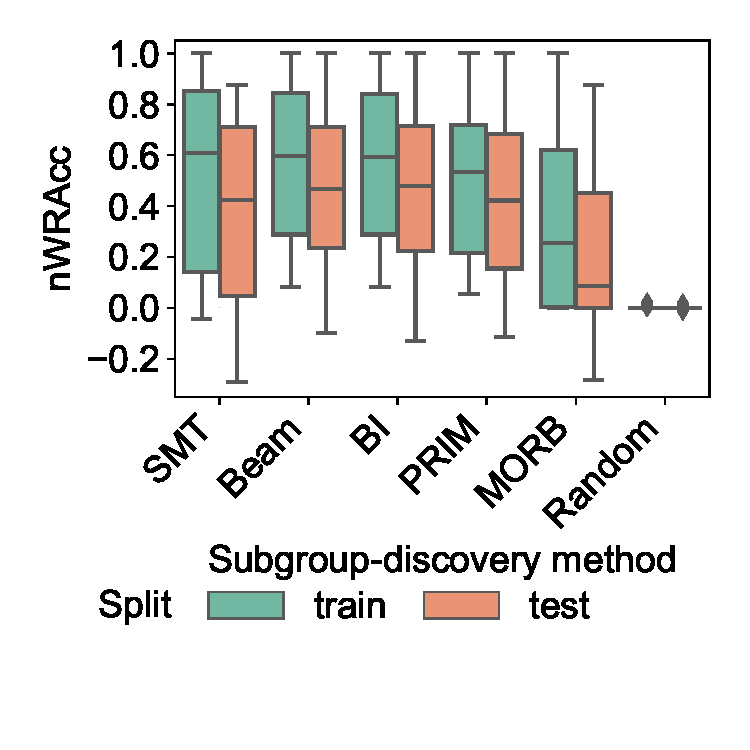
\includegraphics[width=\textwidth, trim=20 60 15 15, clip]{plots/csd-unconstrained-methods-nwracc-all-datasets.pdf}
		\caption{All datasets.}
		\label{fig:csd:unconstrained-methods-nwracc-all-datasets}
	\end{subfigure}
	\hfill
	\begin{subfigure}[t]{0.48\textwidth}
		\centering
		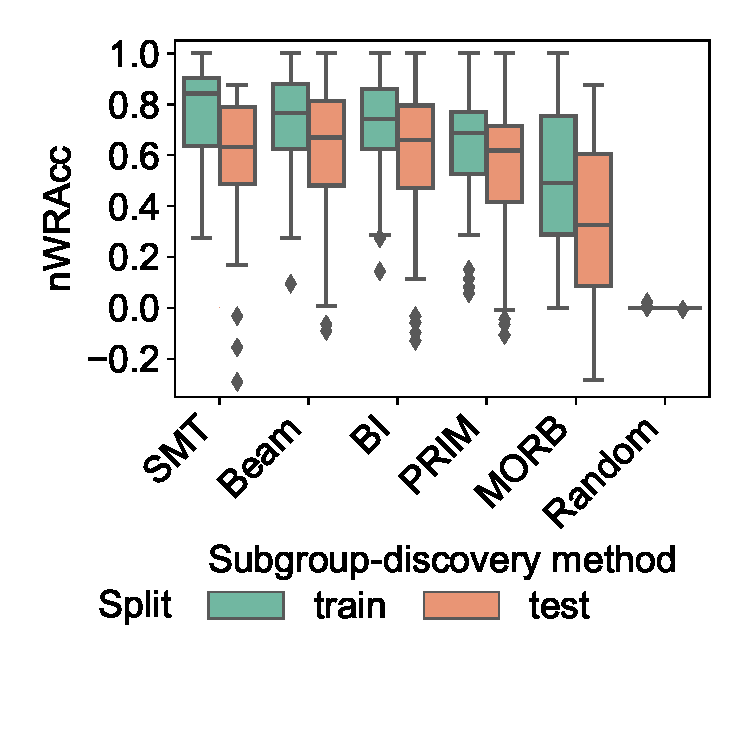
\includegraphics[width=\textwidth, trim=20 60 15 15, clip]{plots/csd-unconstrained-methods-nwracc-no-timeout-datasets.pdf}
		\caption{Datasets without \emph{SMT} timeouts.}
		\label{fig:csd:unconstrained-methods-nwracc-no-timeout-datasets}
	\end{subfigure}
	\caption{
		Subgroup quality (nWRAcc, cf.~Equation~\ref{eq:csd:wracc-normalized}) over datasets and cross-validation folds, by subgroup-discovery method.
		Results from the unconstrained experimental scenario.
	}
	\label{fig:csd:unconstrained-methods-nwracc}
\end{figure}

\paragraph{Subgroup quality}

Figure~\ref{fig:csd:unconstrained-methods-nwracc-all-datasets} compares subgroup quality on the training set and test set for the six subgroup-discovery methods.
On the training set, the two heuristic search methods \emph{Beam} and \emph{BI} have roughly the same median nWRAcc as the solver-based search method \emph{SMT}.
In particular, the heuristics are even better than \emph{SMT} on some datasets but worse on others.
The former can only happen because \emph{SMT} may run into timeouts and therefore not yield the exact optimum, as we analyze later (cf.~Section~\ref{sec:csd:evaluation:timeouts}).
However, even if we limit our analysis to the datasets without \emph{SMT} timeouts, \emph{Beam} and \emph{BI} are still remarkably close to the optimum quality (cf.~Figure~\ref{fig:csd:unconstrained-methods-nwracc-no-timeout-datasets}).
Note that this result is not specific to \emph{SMT} but also holds for any other exhaustive search method.
On the test set, \emph{Beam} and \emph{BI} are even better than \emph{SMT} on median, also excluding timeout datasets, since their training-test nWRAcc difference is smaller.
This result indicates that \emph{Beam} and \emph{BI} are less susceptible to overfitting and their solutions generalize better.
In detail, the average difference between training-set nWRAcc and test-set nWRAcc is 0.125 for \emph{SMT}, 0.101 for \emph{BI}, 0.095 for \emph{Beam}, 0.094 for \emph{MORS}, 0.068 for \emph{PRIM}, and 0.001 for \emph{Random}.

The heuristic search method \emph{PRIM} yields slightly worse subgroup quality than \emph{Beam} and \emph{BI}.
Although it follows an iterative subgroup-refinement procedure like the latter two methods, it is more limited regarding its refinement options.
In particular, \emph{PRIM} always has to remove a fixed fraction~$\alpha$ of data objects from the subgroup, while \emph{Beam} and \emph{BI} can remove more or less data objects.
On the test, \emph{PRIM} yields a median nWRAcc only slightly worse than \emph{SMT}, on all datasets as well as after excluding timeout datasets.

All three heuristic search methods clearly beat the two baselines \emph{MORS} and \emph{Random}.
While \emph{Random} yields the same quality as not restricting the subgroup at all, i.e., an nWRACC of~0, \emph{MORS} is considerably better and therefore a suitable baseline for future studies comparing subgroup-discovery methods.

\begin{table}[t]
	\centering
	\begin{subtable}{\textwidth}
		\centering
		\begin{tabular}{lrrrrrr}
			\toprule
			Aggregate & SMT & Beam & BI & PRIM & MORS & Random \\
			\midrule
			Mean & 855.45~s & 33.03~s & 34.95~s & 1.27~s & 0.01~s & 0.91~s \\
			Standard dev. & 931.85~s & 97.06~s & 103.25~s & 1.54~s & 0.00~s & 1.05~s \\
			Median & 248.88~s & 2.53~s & 2.40~s & 0.69~s & 0.01~s & 0.49~s \\
			\bottomrule
		\end{tabular}
		\caption{
			All datasets.
		}
		\label{tab:csd:unconstrained-runtime-all-datasets}
	\end{subtable}
	\\ \vspace{\baselineskip}
	\begin{subtable}{\textwidth}
		\centering
		\begin{tabular}{lrrrrrr}
			\toprule
			Aggregate & SMT & Beam & BI & PRIM & MORS & Random \\
			\midrule
			Mean & 179.18~s & 11.39~s & 12.36~s & 1.32~s & 0.01~s & 0.86~s \\
			Standard dev. & 295.20~s & 19.82~s & 21.37~s & 1.70~s & 0.00~s & 1.08~s \\
			Median & 57.02~s & 2.53~s & 2.40~s & 0.80~s & 0.01~s & 0.55~s \\
			\bottomrule
		\end{tabular}
		\caption{
			Datasets without \emph{SMT} timeouts.
		}
		\label{tab:csd:unconstrained-runtime-no-timeout-datasets}
	\end{subtable}
	\caption{
		Aggregated runtime over datasets and cross-validation folds, by subgroup-discovery method.
		Results from the unconstrained experimental scenario.
	}
	\label{tab:csd:unconstrained-runtime}
\end{table}

\paragraph{Runtime}

Table~\ref{tab:csd:unconstrained-runtime} summarizes the runtimes of the subgroup-discovery methods.
On average, \emph{SMT} is an order of magnitude slower than \emph{Beam} and \emph{BI}, which are an order of magnitude slower than \emph{PRIM} and the baseline \emph{Random}.
The baseline \emph{MORS} runs in negligible time and therefore is a good tool to obtain a lower bound on subgroup quality instantaneously.
Taking subgroup quality into consideration, the heuristic search methods offer a reasonable quality in a reasonable time, while \emph{SMT} incurs a high cost for its optimal solutions.
Among the three heuristics, \emph{PRIM} is fastest but also yields the lowest subgroup quality, so users should decide which runtime is acceptable.

For \emph{SMT}, the overall runtime not only comprises optimization but also formulating the optimization problem.
Since the latter depends on the dataset size, e.g., involves $O(m)$ constraints with length $O(n)$ each to define the subgroup-membership variables~$b_i$ (cf.~Equation~\ref{eq:csd:smt-constraint-subgroup-membership}), the preparation time can become considerable for large datasets.
In our experiments, formulating the \emph{SMT} problem took 41.4~s on average, with a maximum of 317.6~s.
This average preparation time already is greater than the average total runtime of the heuristics.

\begin{table}[t]
	\centering
	\begin{tabular}{lrrrr}
		\toprule
		Method & $\Sigma n^u$ & $m \cdot n$ & $m$ & $n$ \\
		\midrule
		SMT & 0.40 & 0.72 & 0.69 & 0.22 \\
		Beam & 0.96 & 0.48 & 0.29 & 0.66 \\
		BI & 0.96 & 0.52 & 0.33 & 0.67 \\
		PRIM & 0.84 & 0.57 & 0.31 & 0.76 \\
		MORS & 0.54 & 0.52 & 0.41 & 0.46 \\
		Random & 0.60 & 0.71 & 0.44 & 0.76 \\
		\bottomrule
	\end{tabular}
	\caption{
		Spearman correlation between runtime and metrics for dataset size,
		over datasets and cross-validation folds, by subgroup-discovery method.
		Results from the unconstrained experimental scenario, using datasets without \emph{SMT} timeouts.
	}
	\label{tab:csd:unconstrained-runtime-correlation}
\end{table}

To determine which factors influence runtime, we analyze the Spearman correlation between runtime and four simple metrics for dataset size.
In particular, Table~\ref{tab:csd:unconstrained-runtime-correlation} considers the number of data objects~$m$, the number of features~$n$, the product of these two quantities~$m \cdot n$, and the number of unique values per feature summed over the features~$\Sigma n^u$.
For the three heuristic search methods, the latter metric shows a high correlation to runtime, while \emph{SMT} exhibits the highest runtime correlation to~$m \cdot n$.

\subsection{Solver Timeouts}
\label{sec:csd:evaluation:timeouts}

In this section, we evaluate the impact of solver timeouts for \emph{SMT} search.

\begin{figure}[t]
	\centering
	\begin{subfigure}[t]{0.48\textwidth}
		\centering
		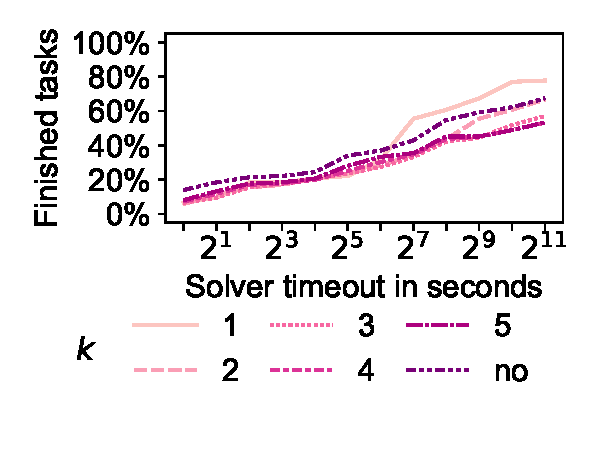
\includegraphics[width=\textwidth, trim=15 25 15 10, clip]{plots/csd-timeouts-finished-tasks.pdf}
		\caption{
			Frequency of finished \emph{SMT} tasks by feature-cardinality threshold~$k$.
		}
		\label{fig:csd:timeouts-finished-tasks}
	\end{subfigure}
	\hfill
	\begin{subfigure}[t]{0.48\textwidth}
		\centering
		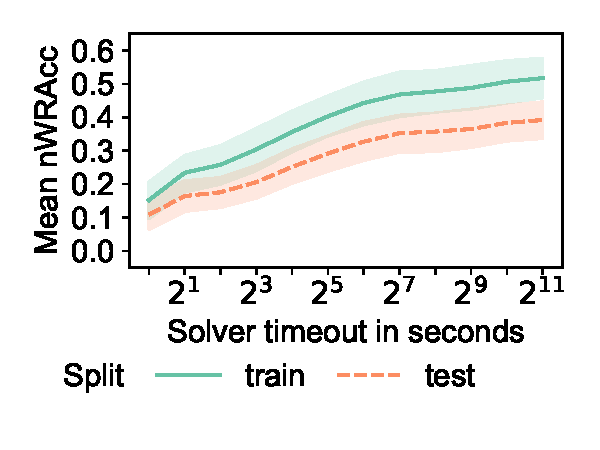
\includegraphics[width=\textwidth, trim=15 25 15 10, clip]{plots/csd-timeouts-nwracc.pdf}
		\caption{
			Mean subgroup quality with 95\% confidence intervals based on datasets and cross-validation folds.
			Results from the unconstrained experimental scenario.
		}
		\label{fig:csd:timeouts-nwracc}
	\end{subfigure}
	\caption{
		Impact of solver timeouts for \emph{SMT} as the subgroup-discovery method.
		Results from the search for original subgroups.
	}
	\label{fig:csd:timeouts}
\end{figure}

\paragraph{Finished tasks}

Figure~\ref{fig:csd:timeouts-finished-tasks} graphs how many of the \emph{SMT} optimization tasks for original subgroups finished within the evaluated solver timeouts.
Besides the unconstrained tasks, we also consider tasks with different feature-cardinality thresholds, though the overall trend is the same.
In particular, the number of finished tasks only increases slowly over time and some tasks take orders of magnitude longer than others.
E.g., in the unconstrained experimental scenario, 19.3\% of the \emph{SMT} tasks finished within 4~s, 25.9\% within 16~s, 36.3\% within 64~s, 55.6\% within 256~s, and 63.0\% within 1024~s.
For the maximum timeout setting of 2048~s, 68.9\% of the \emph{SMT} tasks finished and 17 out of 27 datasets did not encounter timeouts (cf.~Table~\ref{tab:csd:datasets}).

\paragraph{Subgroup quality}

Figure~\ref{fig:csd:timeouts-nwracc} visualizes the subgroup quality over solver timeouts for unconstrained \emph{SMT} search.
This plot shows the quality of the optimal solution for finished tasks and of the currently best solution for unfinished tasks.
As for the number of finished tasks (cf.~Figure~\ref{fig:csd:timeouts-finished-tasks}), the largest gains occur in the first minute.
E.g., the mean test-set nWRAcc over datasets and cross-validation folds is 0.11 for 1~s, 0.18 for 4~s, 0.25 for 16~s, 0.33 for 64~s, and 0.39 for the maximum timeout of 2024~s.
The main cause for this trend is that if a task finishes within a certain timeout, its quality cannot improve for higher timeouts, and a considerable number of tasks does finish relatively early indeed (cf.~Figure~\ref{fig:csd:timeouts-finished-tasks}).
In contrast, if we only consider the tasks where the solver did not finish even within the maximum timeout, the quality increase of the currently best solution over time is marginal.

Further, even \emph{SMT} with a timeout does not compare favorable to fast heuristic search methods.
E.g., with a solver timeout of 64~s, corresponding to an average overall runtime of 89~s, \emph{SMT} achieves a mean training-set nWRAcc of 0.44, compared to 0.56 for \emph{Beam} with an average runtime of 33~s (cf.~Table~\ref{tab:csd:unconstrained-runtime-all-datasets}).

Finally, note that setting a lower solver timeout decreases overfitting, i.e., the difference between training-set nWRAcc and test-set nWRAcc increases over time (cf.~Figure~\ref{fig:csd:timeouts-nwracc}).
However, since the test-set nWRAcc still increases with the timeout as well, choosing lower timeouts does not help quality-wise.

\subsection{Feature-Cardinality Constraints}
\label{sec:csd:evaluation:cardinality}

In this section, we compare all six subgroup-discovery methods in an experimental scenario with feature-cardinality constraints.
The solver-based search method \emph{SMT} uses its default maximum timeout of 2048~s.

\begin{figure}[t]
	\centering
	\begin{subfigure}[t]{0.48\textwidth}
		\centering
		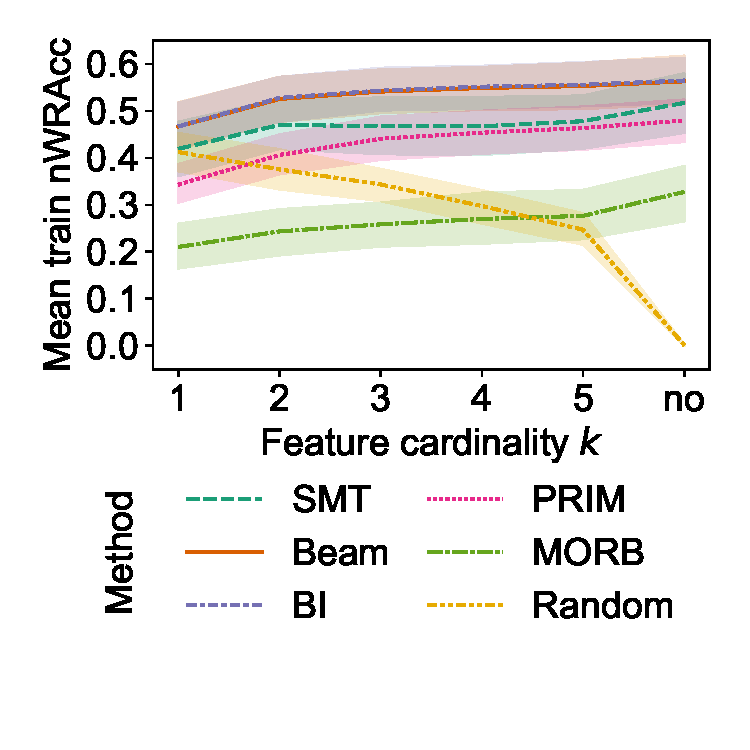
\includegraphics[width=\textwidth, trim=20 60 15 15, clip]{plots/csd-cardinality-methods-train-nwracc.pdf}
		\caption{Training set.}
		\label{fig:csd:cardinality-methods-train-nwracc}
	\end{subfigure}
	\hfill
	\begin{subfigure}[t]{0.48\textwidth}
		\centering
		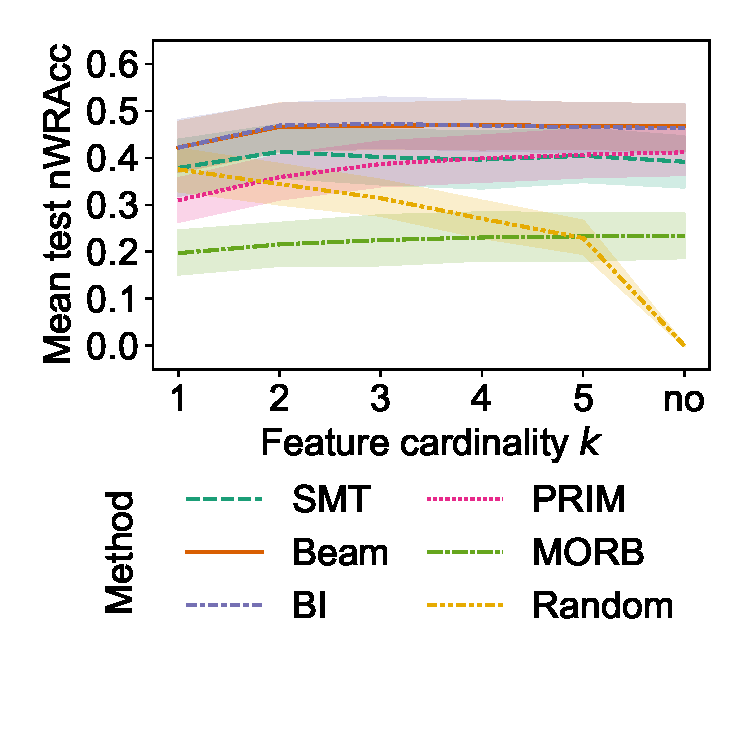
\includegraphics[width=\textwidth, trim=20 60 15 15, clip]{plots/csd-cardinality-methods-test-nwracc.pdf}
		\caption{Test set.}
		\label{fig:csd:cardinality-methods-test-nwracc}
	\end{subfigure}
	\caption{
		Mean subgroup quality with 95\% confidence intervals based on datasets and cross-validation folds, over feature-cardinality threshold~$k$, by subgroup-discovery method.
		Results from the search for original subgroups.
	}
	\label{fig:csd:cardinality-methods-nwracc}
\end{figure}

\paragraph{Subgroup quality}

Figure~\ref{fig:csd:cardinality-methods-nwracc} displays the mean subgroup quality, averaging over datasets and cross-validation folds, for different values of the feature-cardinality threshold~$k$.
For most subgroup-discovery methods, mean training-set nWRACC (cf.~Figure~\ref{fig:csd:cardinality-methods-train-nwracc}) increases with~$k$, though the marginal utility decreases.
In particular, even with $k=1$, the mean nWRAcc is already clearly above 50\% of the nWRAcc achieved without a feature-cardinality constraint.
Further, the quality increase between $k=1$ and $k=2$ is usually the largest.
On the test set (cf.~Figure~\ref{fig:csd:cardinality-methods-test-nwracc}), the benefit of setting a larger~$k$ is even smaller.
E.g., the mean test-set nWRAcc of \emph{Beam}, \emph{BI}, and \emph{SMT} barely improves beyond $k=2$.
These results indicate that sparse subgroup descriptions, which tend to be more interpretable, already yield a high subgroup quality.

The baseline \emph{Random} differs from the other subgroup-discovery methods since its subgroup quality clearly decreases over~$k$.
This behavior results from \emph{Random}'s design (cf.~Algorithm~\ref{al:csd:random-search}).
In particular, it randomly samples bounds independently for each feature.
Thus, each feature excludes a certain fraction of data objects from the subgroup.
The more features are used in the subgroup description, the smaller becomes the expected number of data objects in the subgroup.
Since the number of subgroup members is one factor in WRAcc (cf.~Equation~\ref{eq:csd:wracc}), quality naturally decreases for smaller subgroups.

Figure~\ref{fig:csd:cardinality-methods-nwracc} also reveals that the heuristic search methods \emph{Beam} and \emph{BI} still yield higher average subgroup quality than the solver-based search \emph{SMT} with timeouts, for any feature-cardinality setting.
Further, the heuristic \emph{PRIM} exhibits a larger increase of subgroup quality over~$k$ than \emph{Beam} and \emph{BI}, thereby narrowing the quality gap to the latter.
The baseline \emph{MORS} displays the least effect of~$k$ on mean test-set nWRAcc, showing very stable subgroup quality.

Finally, the results indicate that limiting~$k$ reduces overfitting.
For example, for \emph{Beam}, the mean difference between training-set and test-set nWRAcc is 0.095 without a feature-cardinality constraint, 0.073 for $k=3$, and 0.045 for $k=1$.
The increasing tendency to overfit with larger~$k$ explains why mean training-set nWRAcc increases more than mean test-set nWRAcc over~$k$ in Figure~\ref{fig:csd:cardinality-methods-nwracc}.
From the six subgroup-discovery methods, \emph{PRIM} shows the smallest increase of overfitting over~$k$, \emph{MORS} and \emph{SMT} the largest.

\begin{table}[t]
	\centering
	\begin{tabular}{lrrrrrr}
		\toprule
		$k$ & BI & Beam & MORS & PRIM & Random & SMT \\
		\midrule
		1 & 8.02~s & 7.12~s & 0.01~s & 0.08~s & 0.66~s & 640.79~s \\
		2 & 11.89~s & 10.44~s & 0.01~s & 0.17~s & 0.66~s & 911.66~s \\
		3 & 14.53~s & 13.23~s & 0.01~s & 0.25~s & 0.68~s & 1079.53~s \\
		4 & 16.88~s & 15.21~s & 0.01~s & 0.35~s & 0.68~s & 1128.76~s \\
		5 & 18.82~s & 16.87~s & 0.01~s & 0.46~s & 0.70~s & 1128.38~s \\
		no & 34.95~s & 33.03~s & 0.01~s & 1.27~s & 0.91~s & 855.45~s \\
		\bottomrule
	\end{tabular}
	\caption{
		Mean runtime over datasets and cross-validation folds, by subgroup-discovery method and feature-cardinality threshold~$k$.
		Results from the search for original subgroups.
	}
	\label{tab:csd:cardinality-runtime}
\end{table}

\paragraph{Runtime}

As Table~\ref{tab:csd:cardinality-runtime} displays, the heuristic search methods \emph{Beam}, \emph{BI}, and \emph{PRIM} become faster the smaller~$k$ is.
The baseline \emph{Random} shows a similar trend, though less prominent, while \emph{MORS} yields results instantaneously in any case.
In contrast, the picture for the solver-based search method \emph{SMT} is less clear.
While its average runtime clearly increases over~$k$ till $k=4$, it remains constant for $k=5$ and even decreases without a feature-cardinality constraint, though remaining higher than for $k \leq 2$.

\subsection{Alternative Subgroup Descriptions}
\label{sec:csd:evaluation:alternatives}

In this section, we analyze alternative subgroup descriptions for the subgroup-discovery methods \emph{Beam} and \emph{SMT}.
The solver-based search method \emph{SMT} uses its default maximum timeout of 2048~s.
Both search methods employ a feature-cardinality threshold of~$k=3$.


\begin{figure}[t]
	\centering
	\begin{subfigure}[t]{0.48\textwidth}
		\centering
		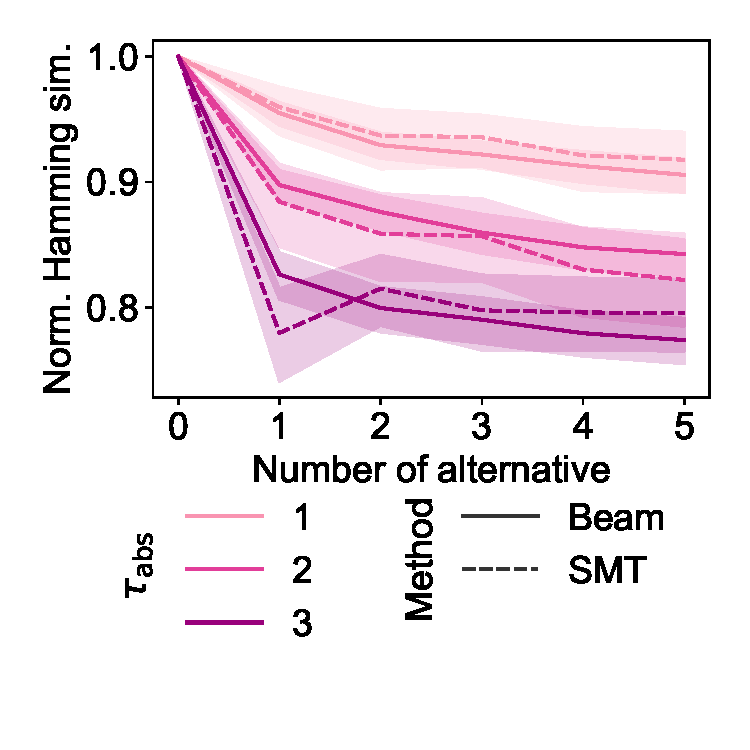
\includegraphics[width=\textwidth, trim=20 50 15 15, clip]{plots/csd-alternatives-similarity-hamming.pdf}
		\caption{Normalized Hamming similarity.}
		\label{fig:csd:alternatives-similarity-hamming}
	\end{subfigure}
	\hfill
	\begin{subfigure}[t]{0.48\textwidth}
		\centering
		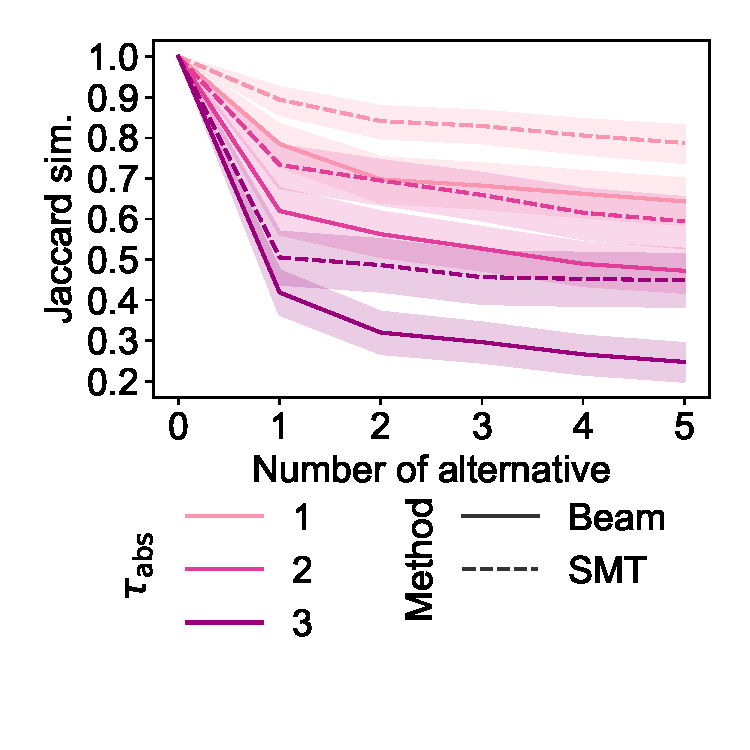
\includegraphics[width=\textwidth, trim=20 50 15 15, clip]{plots/csd-alternatives-similarity-jaccard.pdf}
		\caption{Jaccard similarity.}
		\label{fig:csd:alternatives-similarity-jaccard}
	\end{subfigure}
	\caption{
		Mean subgroup similarity of alternative subgroup descriptions to the original subgroup with 95\% confidence intervals based on datasets and cross-validation folds, over the number of alternatives, by subgroup-discovery method and dissimilarity threshold~$\tau_{\text{abs}}$.
	}
	\label{fig:csd:alternatives-similarity}
\end{figure}

\paragraph{Subgroup similarity}

Figure~\ref{fig:csd:alternatives-similarity} visualizes the average similarity between the original subgroup and the subgroups induced by alternative subgroup descriptions.
As one would expect, the subgroup similarity decreases the more alternatives one desires and the more the selected features in subgroup descriptions should differ.
Further, the decrease is strongest from the original subgroup, i.e., the zeroth alternative, to the first alternative but smaller beyond.
This observation indicates that one may find several alternative subgroup descriptions of comparable similarity to the original.

These trends holds for both similarity measures, i.e., the normalized Hamming similarity we use as optimization objective (cf.~Equation~\ref{eq:csd:hamming-general} and Figure~\ref{fig:csd:alternatives-similarity-hamming}) as well as the Jaccard similarity (cf.~Equation~\ref{eq:csd:jaccard} and Figure~\ref{fig:csd:alternatives-similarity-jaccard}).
The latter yields lower similarity values than the former since it ignores data objects that are not contained in either of the two compared subgroups.
Further, the observed trends exist for the solver-based search method \emph{SMT} as well as the heuristic search method \emph{Beam}.
\emph{SMT} yields clearly more similar subgroups than \emph{Beam} for the Jaccard similarity, while the normalized Hamming similarity does not show a clear winner.

\begin{figure}[t]
	\centering
	\begin{subfigure}[t]{0.48\textwidth}
		\centering
		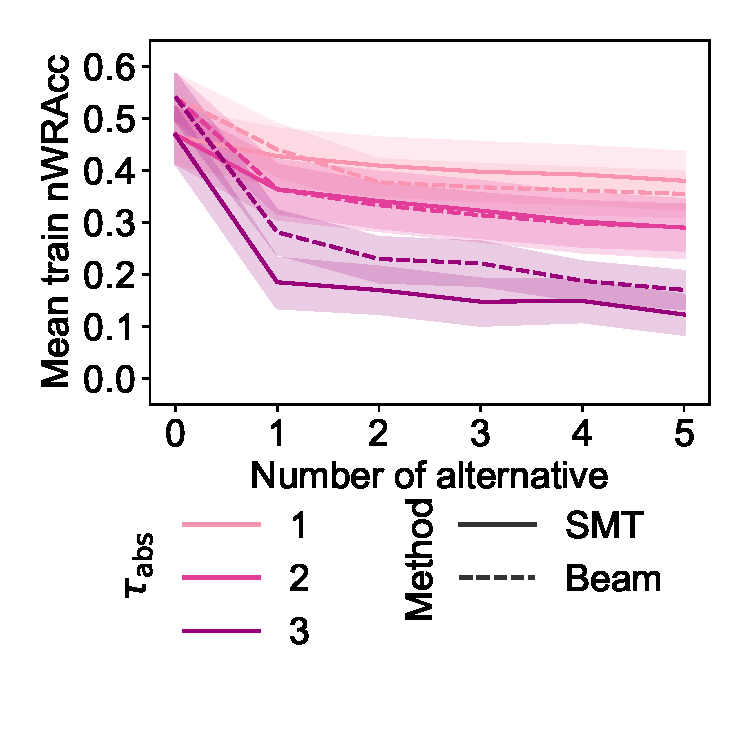
\includegraphics[width=\textwidth, trim=20 50 15 15, clip]{plots/csd-alternatives-train-nwracc.pdf}
		\caption{Training set.}
		\label{fig:csd:alternatives-train-nwracc}
	\end{subfigure}
	\hfill
	\begin{subfigure}[t]{0.48\textwidth}
		\centering
		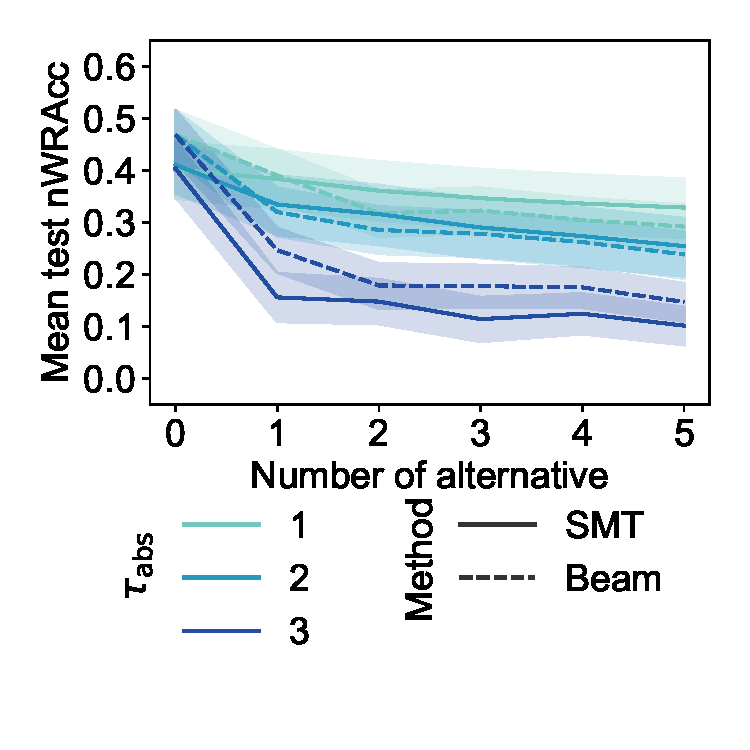
\includegraphics[width=\textwidth, trim=20 50 15 15, clip]{plots/csd-alternatives-test-nwracc.pdf}
		\caption{Test set.}
		\label{fig:csd:alternatives-test-nwracc}
	\end{subfigure}
	\caption{
		Mean subgroup quality with 95\% confidence intervals based on datasets and cross-validation folds, over the number of alternatives, by subgroup-discovery method and dissimilarity threshold~$\tau_{\text{abs}}$.
		Results from the search for alternative subgroup descriptions.
	}
	\label{fig:csd:alternatives-nwracc}
\end{figure}

\paragraph{Subgroup quality}

The average subgroup quality of alternative subgroup descriptions (cf.~Figure~\ref{fig:csd:alternatives-nwracc}) shows similar trends as subgroup similarity (cf.~Figure~\ref{fig:csd:alternatives-similarity}).
In particular, quality decreases over the dissimilarity threshold~$\tau_{\text{abs}}$ and over the number of alternatives~$a$, with the largest decrease to the first alternative.
For the highest dissimilarity threshold~$\tau_{\text{abs}} = 3$, \emph{Beam} consistently yields higher average quality than \emph{SMT} for the original subgroup and each alternative, while the other two values of the dissimilarity threshold do not clearly favor either subgroup-discovery method.
The observed trends on the test set (cf.~Figure~\ref{fig:csd:alternatives-test-nwracc}) are very similar to those on the training set (cf.~Figure~\ref{fig:csd:alternatives-train-nwracc}).
For both subgroup-discovery methods, overfitting as measured by the train-test difference in nWRAcc is lower for the alternative subgroup descriptions than for the original subgroups.
This may be a consequence of the alternative subgroup descriptions not directly optimizing subgroup quality.

\begin{table}[t]
	\centering
	\begin{tabular}{llrrrrrr}
		\toprule
		\multirow{2}{*}{Method} & \multirow{2}{*}{$\tau_{\text{abs}}$} & \multicolumn{6}{c}{Number of alternative} \\
		\cmidrule(lr){3-8}
		& &  0 & 1 & 2 & 3 & 4 & 5 \\
		\midrule
		\multirow[t]{3}{*}{Beam} & 1 & 13.2~s & 8.3~s & 7.9~s & 7.9~s & 7.7~s & 7.6~s \\
		& 2 & 13.3~s & 7.9~s & 7.6~s & 7.5~s & 7.2~s & 7.0~s \\
		& 3 & 13.4~s & 6.1~s & 5.2~s & 4.8~s & 4.1~s & 3.5~s \\
		\multirow[t]{3}{*}{SMT} & 1 & 1079.5~s & 158.7~s & 198.7~s & 219.3~s & 237.2~s & 283.0~s \\
		& 2 & 1100.3~s & 410.8~s & 477.2~s & 527.9~s & 637.2~s & 662.4~s \\
		& 3 & 1104.2~s & 913.4~s & 693.2~s & 629.2~s & 616.7~s & 577.9~s \\
		\bottomrule
	\end{tabular}
	\caption{
		Mean runtime over datasets and cross-validation folds, by subgroup-discovery method, dissimilarity threshold~$\tau_{\text{abs}}$, and number of alternative.
		Results from the search for alternative subgroup descriptions.
	}
	\label{tab:csd:alteratives-runtime}
\end{table}

\paragraph{Runtime}

Table~\ref{tab:csd:alteratives-runtime} displays the average runtime for searching original subgroups and alternative subgroup descriptions.
The search for alternatives is faster for both analyzed search methods, i.e., \emph{Beam} and \emph{SMT}.
As for the original subgroups, \emph{Beam} search for alternative subgroup descriptions is one to two orders magnitude faster than the solver-based \emph{SMT} search.
For \emph{Beam}, runtime tends to decrease over the number of alternatives, while \emph{SMT} shows less clear behavior.
In particular, its runtime increases over alternatives for~$\tau_{\text{abs}} \in \{1, 2\}$, i.e., settings that allow reusing features from previous subgroup descriptions.
In contrast, runtime decreases over alternatives for $\tau_{\text{abs}} = k = 3$, which forbids selecting any feature used in a previous subgroup description.
Finally, the number of \emph{SMT} tasks finished within the solver timeout shows trends corresponding to the runtime.
In particular, there are more finished tasks when searching for alternative subgroup descriptions rather than original subgroups.

\subsection{Summary}
\label{sec:csd:evaluation:summary}

\paragraph{Unconstrained subgroup discovery (cf.~Section~\ref{sec:csd:evaluation:unconstrained})}

We recommend using heuristic search methods rather than solver-based search.
In particular, \emph{Beam} and \emph{BI} were an order of magnitude faster than \emph{SMT} and still yielded higher test-set subgroup quality since they were less prone to overfitting.
The latter result not only impedes \emph{SMT} but exhaustive algorithmic search methods as well.
\emph{PRIM} was faster than \emph{Beam} and \emph{BI} but yielded lower subgroup quality.
The same insights applied even more to our novel baseline \emph{MORS}, which provided instantaneous, non-trivial lower bounds for subgroup quality.

\paragraph{Solver timeouts (cf.~Section~\ref{sec:csd:evaluation:timeouts})}

Setting larger solver timeouts showed a decreasing marginal utility regarding the number of finished \emph{SMT} tasks and subgroup quality i.e., most gains occurred within the first few seconds or dozens of seconds.
About half the \emph{SMT} tasks that finished at all finished in under a minute.
However, the average training-set subgroup quality for this solver timeout was lower than for heuristic search methods with even lower runtime.

\paragraph{Feature-cardinality constraints (cf.~Section~\ref{sec:csd:evaluation:cardinality})}

Using more features in subgroup descriptions showed a decreasing marginal utility regarding subgroup quality.
For \emph{Beam}, \emph{BI}, and \emph{SMT}, test-set subgroup-quality was already close to the unconstrained scenario at $k=2$, while \emph{PRIM} benefited more from larger~$k$.
A smaller~$k$ made the heuristic search methods faster and generally reduced overfitting.
The baseline \emph{MORS} showed stable test-set subgroup quality regarding~$k$, while \emph{Random} even increased subgroup quality with smaller~$k$.

\paragraph{Alternative subgroup descriptions (cf.~Section~\ref{sec:csd:evaluation:alternatives})}

The heuristic \emph{Beam} was one to two orders of magnitude faster than solver-based \emph{SMT} when searching for alternative subgroup descriptions, while both search methods found alternatives faster than original subgroups.
The quality and similarity of alternative subgroup descriptions strongly depended on two user parameters, i.e., the number of alternatives~$a$ and the dissimilarity threshold on feature selection~$\tau_{\text{abs}}$.
The quality and similarity difference between the original and the first alternative was higher than among the first few alternatives.

\section{Related Work}
\label{sec:csd:related-work}

In this section, we review related work.
Next to literature on subgroup discovery (cf.~Section~\ref{sec:csd:related-work:subgroup-discovery}), we also discuss relevant work from the adjacent field of feature selection (cf.~Section~\ref{sec:csd:related-work:feature-selection}) and other related areas (cf.~Section~\ref{sec:csd:related-work:other}).

\subsection{Subgroup Discovery}
\label{sec:csd:related-work:subgroup-discovery}

In this section, we present related work from the field of subgroup discovery.
First, we discuss algorithmic search methods (cf.~Section~\ref{sec:csd:related-work:subgroup-discovery:algorithmic-methods}) as well as white-box formulations (cf.~Section~\ref{sec:csd:related-work:subgroup-discovery:white-box}) for this problem.
Second, we cover constrained subgroup discovery in general (cf.~Section~\ref{sec:csd:related-work:subgroup-discovery:constraints}) and for the two constraint types we focus on, i.e., feature-cardinality constraints (cf.~Section~\ref{sec:csd:related-work:subgroup-discovery:cardinality}) and alternative subgroup descriptions (cf.~Section~\ref{sec:csd:related-work:subgroup-discovery:alternatives}).

\subsubsection{Algorithmic Search Methods}
\label{sec:csd:related-work:subgroup-discovery:algorithmic-methods}

Nearly all existing subgroup-discovery methods are algorithmic.
In particular, there are heuristic search methods like PRIM~\cite{friedman1999bump} and BI~\cite{mampaey2012efficient} as well as exhaustive search methods, potentially with pruning to cut down the search space, like SD-Map~\cite{atzmueller2009fast, atzmueller2006sd}, MergeSD~\cite{grosskreutz2009subgroup}, and BSD~\cite{lemmerich2016fast, lemmerich2010fast}.
See~\cite{atzmueller2015subgroup, helal2016subgroup, herrera2011overview, ventura2018subgroup} for surveys of subgroup-discovery methods.
To the best of our knowledge, optimizing subgroup discovery with an SMT solver is novel.
There are a few other white-box formulations of particular variants of subgroup discovery, which differ from our work in several aspects, as we discuss in the following.

\subsubsection{White-Box Formulations}
\label{sec:csd:related-work:subgroup-discovery:white-box}

\paragraph{Maximum box problem}

\cite{eckstein2002maximum}~formulates an integer program for the \textsc{Maximum Box} problem, which is about finding a hyperrectangle containing as many positive data objects as possible but no negative data objects, i.e., no false positives.
This problem is an intermediate between subgroup discovery (cf.~Definition~\ref{def:csd:subgroup-discovery}), which allows false positives and false negatives, and perfect-subgroup discovery (cf.~Definition~\ref{def:csd:perfect-subgroup-discovery}), which allows neither.
Also, it has some similarity to minimal-optimal-recall-subgroup discovery (cf.~Definition~\ref{def:csd:minimal-optimal-recall-subgroup-discovery}), which is about finding a subgroup with as \emph{few negative} data objects as possible but \emph{all positive} data objects.
While the latter problem is in~$\mathcal{P}$ (cf.~Proposition~\ref{prop:csd:complexity-unconstrained-minimal-optimal-recall-subgroup-discovery}), \cite{eckstein2002maximum}~proves $\mathcal{NP}$-hardness of the \textsc{Maximum Box} problem by reduction from the \textsc{Maximum Independent Set}~\cite{tarjan1977finding} problem.
In their evaluation, the authors only use a customized branch-and-bound algorithm but neither solver-based search nor heuristic search methods.
Further, they consider neither feature-cardinality constraints nor alternative descriptions.

\paragraph{Maximum $\alpha$ pattern problem}

\cite{bonates2008maximum}~investigates the \textsc{Maximum $\alpha$-Pattern} problem.
This problem is similar to the \textsc{Maximum Box} problem but involves a binary dataset and requires a user-selected data object~$\alpha$ to be member of the subgroup.
Again, cardinality constraints or alternative descriptions are not considered.
The authors formulate two integer programs as well as two heuristics.
They evaluate their approaches, but no existing subgroup-discovery methods, on generated and benchmark datasets, comparing subgroup quality as well as runtime.
Similar to us, they find that heuristics  may reach a subgroup quality similar to a solver-based search with orders of magnitude less runtime.

\paragraph{Box search problem}

\cite{louveaux2014combinatorial}~proposes two integer-programming formulation for the \textsc{Box Search} problem, which is about finding a hyperrectangle that optimizes the sum of the target variable of all contained data objects.
In particular, the target variable is continuous rather than binary and the chosen objective differs from ours.
Further, there are no constraints on feature cardinality or for alternative descriptions.
In their evaluation, the authors compare solver-based search to multiple versions of a new branch-and-bound approach but not heuristic search methods.
They use synthetically generated datasets rather than typical machine-learning benchmark datasets.

\paragraph{Closed discriminative itemset mining problem}

Besides five other related problems, \cite{koccak2020exploiting}~formulates \textsc{Closed Discriminative Itemset Mining} with the constraint-specification language \emph{Essence}~\cite{frisch2008ssence}.
In particular, this formulation is close to frequent itemset mining, where items correspond to binary features and the subgroup description is an itemset.
There is no optimization objective but constraints on the frequency of itemsets and on their relevance, excluding dominated solutions.
The authors propose a transformation of their problem specification to enable using standard propositional-satisfiability (SAT) or constraint-programming (CP) solvers.
Their evaluation exclusively analyzes solver runtime rather than subgroup quality and does not compare against heuristic search methods.
Finally, they do not search for alternative descriptions and instead of feature-cardinality constraints, they randomly generate costs and values for items and according lower and upper bounds for itemsets.

\cite{guns2011itemset} also provides a constraint-programming formulation of \textsc{Discriminative Itemset Mining}.
The authors compare two configurations of a constraint solver against two existing itemset-mining algorithms.
They evaluate runtime but not quality, as they enumerate all non-redundant itemsets, and do not include constraints for feature cardinality or alternative descriptions.

\subsubsection{Constrained Subgroup Discovery}
\label{sec:csd:related-work:subgroup-discovery:constraints}

Section~\ref{sec:csd:approach:constraint-types} has already discussed various constraint types in subgroup discovery.
Typically, constraints are not formulated declaratively for solver-based optimization but integrated into algorithmic search methods.
\cite{atzmueller2007using}~expresses domain knowledge with the logic programming language Prolog, creating a knowledgebase composed of facts and rules.
However, the authors do not use a solver to optimize subgroup discovery.

In the following, we discuss particular related work for the two constraint types we analyze in detail.

\subsubsection{Feature-Cardinality Constraints}
\label{sec:csd:related-work:subgroup-discovery:cardinality}

\paragraph{Formulation}

Feature cardinality is a common constraint type~\cite{meeng2021real} and a well-known metric for subgroup complexity~\cite{atzmueller2015subgroup, helal2016subgroup, herrera2011overview, ventura2018subgroup}.
However, our SMT formulation of this constraint type is novel.
\cite{li2015efficient}~formulates a quadratic program to select non-redundant features for subgroups, but this is only a subroutine within an algorithmic search for subgroups.
Also, the authors define a continuous optimization problem with real-valued feature weights as decision variables, while feature selection within our SMT formulation is discrete (cf.~Equation~\ref{eq:csd:smt-constraint-feature-selection}).

\paragraph{Empirical studies}

While several articles on subgroup discovery use a feature-cardinality constraint in their experiments~\cite{arzamasov2022pedagogical, mampaey2012efficient, lavrac2006relevancy, leeuwen2012diverse, leeuwen2013discovering}, there are only few studies that analyze the impact of different feature-cardinality thresholds on different subgroup-discovery methods broadly and systematically.
\cite{friedman1999bump} analyzes the subgroup quality over eliminating a different number of redundant features as a post-processing step for PRIM, but only for one dataset.
\cite{lemmerich2010fast} evaluates different search depths for their algorithm BSD but only regarding runtime and number of subgroups after quality-based pruning, not subgroup quality itself.
\cite{proencca2022robust} compares multiple search depths for their algorithm SSD++, which returns a list of multiple subgroups, regarding an information-theoretic quality measure.
\cite{helal2016subgroup} compares five subgroup-discovery methods with categorical datasets and also evaluates feature cardinality but does not systematically constrain the latter to different values.
\cite{meeng2021real} evaluates three subgroup-discovery methods, including a beam search and an exhaustive search, with numeric datasets.
The authors use feature-cardinality constraints with~$k \in \{1, 2, 3, 4\}$ but mainly focus their evaluation on comparing strategies for handling numeric data.
Also, they only use six datasets, five of them with at most ten features, while we employ more and higher-dimensional datasets.
Additionally, we compare subgroup discovery with feature-cardinality constraints to an unconstrained setting.

\subsubsection{Alternative Subgroup Descriptions}
\label{sec:csd:related-work:subgroup-discovery:alternatives}

To the best of our knowledge, alternative subgroup descriptions in the sense of this paper are a novel concept.
In particular, we aim to maximize the set similarity of contained data objects relative to an original subgroup while using a different subgroup description (cf.~Definition~\ref{def:csd:alternative-subgroup-description-discovery}).
In contrast, there are various existing approaches striving for alternatives in the sense of diverse or non-redundant sets of subgroups, which aim to minimize rather than maximize the overlap of contained data objects~\cite{atzmueller2015subgroup} (cf.~Section~\ref{sec:csd:approach:constraint-types}).
In the following, we discuss approaches that focus on subgroup descriptions.

\paragraph{Description-based diverse subgroup set selection}

\cite{leeuwen2012diverse} introduces six strategies to foster diversity while searching for multiple subgroups simultaneously.
Besides strategies assessing the contained data objects and the compression achieved by subgroups, two strategies refer to the subgroup description.
The first strategy excludes subgroup descriptions that have the same quality and differ in only one condition from an existing subgroup description.
The second strategy uses a global upper bound on how often a feature may be selected in a set of subgroup descriptions rather than controlling pairwise dissimilarity.
Both these strategies give users less control on the overlap of subgroup descriptions than our dissimilarity parameter~$\tau$ does.
Further, \cite{leeuwen2012diverse} targets at simultaneous beam search, optimizing subgroup quality and using the diversity strategies only to prune certain solution candidates.
In contrast, we search for alternative descriptions sequentially, optimize similarity to the original subgroup, and also consider a solved-based search method besides heuristic search.

\paragraph{Diverse top-k characteristics lists}

\cite{lopez2023discovering}~introduces the notion of \emph{diverse top-k characteristic lists}, which is a set of lists each containing multiple patterns, e.g., subgroups.
Within each list, the subgroups should be alternative to each other in terms of data objects contained.
Between lists, subgroup descriptions should be diverse.
However, the latter goal is implemented with a very simple notion of diversity, i.e., exactly the same subgroup description must not appear in two lists but any other overlap is allowed.

\paragraph{Equivalent subgroup descriptions of minimal length}

\cite{boley2009non}~introduces the notion of \emph{equivalent subgroup descriptions of minimal length}, which is stricter than our notion of alternative subgroup descriptions.
In particular, the former descriptions need to cover exactly the same set of data objects, like our notion of perfect alternative subgroup descriptions (cf.~Definition~\ref{def:csd:perfect-alternative}), instead of maximizing similarity.
Further, the original feature set should be minimized, i.e., a subset be found, instead of using a different feature set subject to a dissimilarity constraint.
The authors prove $\mathcal{NP}$-hardness and propose two algorithms for their problem but do not pursue a solver-based search.
We adapt their hardness proof to the perfect-subgroup-discovery problem with a feature-cardinality constraint (cf.~Proposition~\ref{prop:csd:complexity-cardinality-np-perfect-subgroup}), based on which we derive further proofs for problems with feature-cardinality constraints and alternative subgroup descriptions.

\subsection{Feature Selection}
\label{sec:csd:related-work:feature-selection}

Both constraint types we analyze, i.e., feature-cardinality constraints and alternative subgroup descriptions, relate to the features used in the subgroup description.
In the field of feature selection~\cite{guyon2003introduction, li2017feature}, constraints are a topic as well~\cite{bach2023finding, bach2024alternative, bach2022empirical}.
While limiting feature-set cardinality is very common in feature-selection methods, \cite{bach2023finding, bach2024alternative} are unique in that they propose a white-box formulation of alternative feature selection.
Similar to Equation~\ref{eq:csd:smt-constraint-dissimilarity}, they use a threshold-based dissimilarity constraint on feature selection, though with a different dissimilarity measure.
Besides sequential search for alternatives, which we use as well, they also analyze simultaneous search.

Despite the similarities, feature selection generally tackles a fundamentally different optimization problem than subgroup discovery.
In particular, the former problem is `only' about selecting the features instead of also determining bounds on them.
The selected features do not form a prediction model per se but are used in another machine-learning model afterwards.
For feature selection itself, a notion of feature-set quality serves as the objective function.
The latter depends on the feature-selection method but typically assesses features globally, while subgroups describe a particular region in the data.

\subsection{Other Fields}
\label{sec:csd:related-work:other}

\paragraph{Classification}

There are white-box formulations for various types of classification models~\cite{ignatiev2021reasoning}.
E.g., there are formulations in propositional logic (SAT) for optimal decision trees, decision sets, and decision lists~\cite{narodytska2018learning, shati2021sat, yu2021learning}.
Similar to subgroup descriptions, these three model types also use conjunctions of conditions to form decision rules.
Creating sparse models to reduce model complexity, as we do with feature-cardinality constraints, is an issue for such models as well~\cite{yu2021learning}.
However, these model types use multiple rules to classify data globally, while subgroup discovery employs one rule to describe an interesting region.
Further, some of these particular white-box formulations target at perfect predictions rather than optimizing a notion of prediction quality.

\paragraph{Constrained data mining}

\cite{grossi2017survey} provides a broad survey on constraints in various fields of data mining, i.e., classification, clustering, and pattern mining.

\paragraph{Counterfactual explanations}

Searching for counterfactual explanations is an explainable-AI paradigm that targets at data objects with feature values as similar as possible to a given data object but with a different prediction of a given classifier~\cite{guidotti2022counterfactual}.
Thus, counterfactuals provide alternative explanations on the local level, i.e., for individual data objects.
In contrast, alternative subgroup descriptions aim to reproduce subgroup membership globally, striving for a similar prediction but a different feature selection.
Approaches yielding multiple counterfactuals often foster diversity, e.g., by extending the optimization objective~\cite{mothilal2020explaining} or introducing constraints~\cite{karimi2020model, mohammadi2021scaling, russell2019efficient}.
However, only some approaches have a user-friendly parameter to actively control the diversity of solutions.
In particular, \cite{mohammadi2021scaling} offers a dissimilarity threshold comparable to our parameter~$\tau$ for alternative subgroup descriptions.

\paragraph{Redescription mining}

Redescription mining aims to find pairs or sets of descriptions that cover exactly or approximately the same data objects~\cite{galbrun2017redescription, ramakrishnan2004turning}.
Our notion of alternative subgroup descriptions pursues a similarity goal.
However, we search for alternative descriptions sequentially instead of simultaneously.
Also, the original subgroup description usually optimizes subgroup quality, while redescription mining has no target variable, i.e., is unsupervised~\cite{ramakrishnan2004turning}.
Further, redescription mining works with different dissimilarity criteria than we do, e.g., having features pre-partitioned into non-overlapping sets~\cite{galbrun2017redescription, gallo2008finding, mihelcic2023complexity} or requiring only one arbitrary part of the description to differ~\cite{parida2005redescription}.
In contrast, we allow users controlling the overlap between feature sets with the parameter~$\tau$ (cf.~Equation~\ref{eq:csd:smt-constraint-dissimilarity}).
Also, the language for redescriptions may be more complex than for subgroups, e.g., also involve logical negation ($\lnot$) and disjunction ($\lor$)~\cite{galbrun2017redescription, gallo2008finding}, while subgroup descriptions only use the logical AND ($\land$) over features.
Finally, most existing approaches for redescription mining are algorithmic rather than using white-box optimization~\cite{galbrun2017redescription, mihelcic2023complexity}, though~\cite{guns2013kpattern} provides a constraint-programming formulation of this problem and other pattern-set mining problems.
Several formulations and parametrizations of the redescription-mining problem are $\mathcal{NP}$-hard; see \cite{mihelcic2023complexity} for a detailed analysis.

\section{Conclusions and Future Work}
\label{sec:csd:conclusion}

In this section, we recap our article (cf.~Section~\ref{sec:csd:conclusion:conclusion}) and propose directions for future work (cf.~Section~\ref{sec:csd:conclusion:future-work}).

\subsection{Conclusions}
\label{sec:csd:conclusion:conclusion}

Subgroup-discovery methods constitute an important category of interpretable machine-learning models.
In this article, we analyzed constrained subgroup discovery as another step to improve interpretability.
First, we formalized subgroup discovery as an SMT optimization problem.
This formulation supports a variety of user constraints and enables solver-based search for subgroups.
In particular, we studied two constraint types, i.e., limiting the number of features used in subgroups and searching for alternative subgroup descriptions.
For the latter constraint type, we let users control the number of alternatives and a dissimilarity threshold.
We showed how to integrate these constraint types into our SMT formulation as well as existing heuristic search methods for subgroup discovery.
Further, we proved $\mathcal{NP}$-hardness of the optimization problem with constraints.
Finally, we evaluated heuristic and solver-based search with 27 binary-classification datasets.
In particular, we analyzed four experimental scenarios:
unconstrained subgroup discovery, our two constraint types, and timeouts for solver-based search.

\subsection{Future Work}
\label{sec:csd:conclusion:future-work}

\paragraph{Datasets}

Our evaluation used over two dozen generic benchmark datasets (cf.~Section~\ref{sec:csd:experimental-design:datasets}).
While such an evaluation shows general trends, the impact of constraints naturally depends on the dataset.
Thus, our results may not transfer to each particular scenario.
This caveat calls for domain-specific case studies.
In such studies, one could also interpret alternative subgroup descriptions qualitatively, i.e., from the domain perspective.

\paragraph{Constraint types}

We formalized, analyzed, and evaluated two constraint types, i.e., feature-cardinality constraints (cf.~Sections~\ref{sec:csd:approach:cardinality} and~\ref{sec:csd:evaluation:cardinality}) and alternative subgroup descriptions (cf.~Sections~\ref{sec:csd:approach:alternatives} and~\ref{sec:csd:evaluation:alternatives}).
As mentioned in Section~\ref{sec:csd:approach:constraint-types}, there are further constraint types one could investigate, e.g., domain-specific constraints, secondary objectives, or alternatives in the sense of covering different data objects rather than covering the same data objects differently.

For our constraint type for alternative subgroup descriptions, one could analyze other dissimilarities, e.g., symmetric ones rather than the asymmetric one we used (cf.~Equation~\ref{eq:csd:constraint-dissimilarity}).
While the SMT encoding of subgroup discovery is relatively flexible regarding dissimilarities, integrating them into heuristic search methods may be challenging, e.g., if they are not antimonotonic.

\paragraph{Formalization}

In solver-based search for subgroups, we used an SMT encoding (cf.~Section~\ref{sec:csd:approach:smt}) and one particular solver.
Different white-box encodings or solvers may speed up the search and lead to less timeouts, potentially improving the subgroup quality.
We already proposed MILP and MaxSAT encodings of subgroup discovery (cf.~Appendix~\ref{sec:csd:appendix:further-encodings}), though without evaluation.

Two assumptions for subgroup discovery in our article were numerical features and a binary target (cf.~Section~\ref{sec:csd:fundamentals:problem}).
One could adapt the SMT encoding to multi-valued categorical features (cf.~Appendix~\ref{sec:csd:appendix:further-encodings}) and continuous targets.

\paragraph{Computational complexity}

We established $\mathcal{NP}$-hardness for optimizing subgroups with a feature-cardinality constraint (cf.~Propositions~\ref{prop:csd:complexity-cardinality-np-perfect-subgroup} and~\ref{prop:csd:complexity-cardinality-np}).
While the search problem admits a polynomial-time algorithm for perfect subgroups without such constraints (cf.~Proposition~\ref{prop:csd:complexity-unconstrained-perfect-subgroup}), we did not analyze the general unconstrained optimization problem, i.e., including imperfect subgroups.

Further, we showed $\mathcal{NP}$-hardness for finding alternative subgroup descriptions for perfect and imperfect subgroups (cf.~Propositions~\ref{prop:csd:complexity-perfect-alternatives-np-perfect-subgroup} and~\ref{prop:csd:complexity-perfect-alternatives-np-imperfect-subgroup}).
In both cases, our proofs tackle perfect alternatives (cf.~Definition~\ref{def:csd:perfect-alternative}), i.e., alternative descriptions that entail exactly the same subgroup membership of data objects as the original subgroup.
One could try to extend these proofs to imperfect alternatives.
Also, our proofs focused on scenarios where all originally selected features must not be selected in the alternative subgroup description, i.e., a specific value of dissimilarity threshold~$\tau$.
One could analyze scenarios with overlapping feature sets explicitly.

Regarding parameterized complexity for the unconstrained scenario, feature-cardinality constraints, and alternative subgroup descriptions, we proved membership in the relatively broad complexity class $\mathcal{XP}$ (cf.~Propositions~\ref{prop:csd:complexity-unconstrained-xp}, \ref{prop:csd:complexity-cardinality-xp}, and~\ref{prop:csd:complexity-alternatives-xp}).
One may attempt to tighten these results.

Finally, while we described how one can integrate feature-cardinality constraints and alternative subgroup descriptions into heuristic search methods (cf.~Sections~\ref{sec:csd:approach:cardinality:heuristics} and~\ref{sec:csd:approach:alternatives:heuristics}), we did not provide quality guarantees relative to the exact optimum.
In that regard, one could seek for an approximation complexity result, e.g., membership in the complexity class~$\mathcal{APX}$.

%~\\
%\noindent \textsc{Acknowledgments}\quad
%This work was supported by the Ministry of Science, Research and the Arts Baden-Württemberg, project \emph{Algorithm Engineering for the Scalability Challenge (AESC)}.

\appendix

\section{Appendix}
\label{sec:csd:appendix}

In this section, we provide supplementary materials.
Appendix~\ref{sec:csd:appendix:further-encodings} describes further encodings of the subgroup-discovery problem, complementing the SMT encoding from Section~\ref{sec:csd:approach:smt}.
Appendix~\ref{sec:csd:appendix:proofs} contains proofs for propositions from Section~\ref{sec:csd:approach}.

\subsection{Further Problem Encodings of Subgroup Discovery}
\label{sec:csd:appendix:further-encodings}

In this section, we provide additional encodings of subgroup-discovery as a white-box optimization problem.
First, we describe how to encode categorical features within the SMT formulation (cf.~Section~\ref{sec:csd:appendix:further-encodings:smt-categorical}).
Next, we discuss encodings as a mixed-integer linear program (cf.~Section~\ref{sec:csd:appendix:further-encodings:milp}) and a maximum-satisfiability problem (cf.~Section~\ref{sec:csd:appendix:further-encodings:max-sat}).

\subsubsection{Handling Categorical Features in SMT Encoding}
\label{sec:csd:appendix:further-encodings:smt-categorical}

In general, there are many different options to numerically encode categorical data in machine learning~\cite{matteucci2023benchmark}.
Similarly, there are also multiple options to consider categorical features in the SMT formulation of subgroup discovery.
We present three of them in the following.

\paragraph{Two variables per categorical feature}

As a straightforward option, one may map all categories, i.e., unique values, of each categorical feature to distinct integers before instantiating the optimization problem.
This so-called ordinal encoding allows us to directly apply our existing SMT formulation (cf.~Equation~\ref{eq:csd:smt-problem-unconstrained-complete}) to the dataset, at least technically.
Consequently, there are two integer-valued bound variables for each encoded categorical feature.
However, the ordering of categories should be semantically meaningful since it influences which categories may jointly be included in the subgroup.
In particular, only sets of categories that form contiguous integer ranges in the ordinal encoding may define subgroup membership.
I.e., the subgroup may comprise the encoded categories~$\{3,4,5\}$, but not only~$\{3,5 \}$ since it needs to include all values between a lower and an upper bound.
If there is no meaningful ordering of categories, one should choose a different encoding.

\paragraph{Two variables per categorical feature value}

One can achieve more flexibility by introducing separate bound variables for each category of a feature rather than only for each feature.
This approach corresponds to a one-hot encoding of the dataset, which creates one new binary feature for each category.
Thus, the bound variables effectively are binary as well.
By default in our SMT encoding, there is a logical AND ($\land$) over the binary features, i.e., categories.
The interpretation of bound values for one binary Feature~$j$ is as follows:

(Case 1) $\mathit{lb}_j = \mathit{ub}_j = 1$ means that data objects that assume the corresponding category for Feature~$j$ are members of the subgroup.
This case should apply to at most one category of each feature.
Otherwise, the AND operator would require each data object to assume multiple categories for one feature, which is unsatisfiable.
Thus, this encoding cannot directly express that a set of categories is included the subgroup.

(Case 2) $\mathit{lb}_j = \mathit{ub}_j = 0$ means that data objects that do \emph{not} assume the corresponding category for Feature~$j$ are members of the subgroup.
I.e., data objects assuming the corresponding category are not members of the subgroup.
Other than Case~1, this case can apply to multiple categories of each feature, i.e., the subgroup may directly exclude multiple categories.
Further, if one category is actively included in the subgroup, i.e., falls into Case~1, then Case-2 bounds on other categories are redundant since they are implied by the former.

(Case 3) $\mathit{lb}_j = 0,~\mathit{ub}_j = 1$ explicitly deselects a binary feature, i.e., both binary values do not restrict subgroup membership.

(Case 4) $\mathit{lb}_j = 1,~\mathit{ub}_j = 0$ cannot occur since it violates the bound constraints (cf.~Equation~\ref{eq:csd:smt-constraint-bounds-monotonic}).

Finally, note that binary features allow us to slightly simplify the subgroup-membership expression (cf.~Equation~\ref{eq:csd:smt-constraint-subgroup-membership}).
In general, we need to check lower bound and upper bound for a feature.
However, if a binary feature assumes the value~0 for a data object, checking the upper bound is unnecessary since it is always satisfied.
Similarly, if a binary feature assumes the value~1 for a data object, checking the lower bound is unnecessary since it is always satisfied.
Both these simplifications assume that the bounds are explicitly defined as binary or at least in $[0, 1]$, which can be enforced with straightforward constraints.
Otherwise, the bounds may theoretically be placed outside the feature's range and exclude all data objects, producing an empty subgroup.

\paragraph{One variable per categorical feature value}

In some scenario, it does not make sense to include the absence of a category in the subgroup, i.e., to permit $\mathit{lb}_j = \mathit{ub}_j = 0$.
In particular, some existing subgroup-discovery methods for categorical data assume that only the presence of categories is interesting~\cite{atzmueller2015subgroup}.
In this case, introducing one instead of two bound variable(s) for each category suffices.
Assume the categorical Feature~$j$ has $|c_j| \in \mathbb{N}$ different categories~$\{c^1_j, \dots, c^{|c_j|}_j\}$.
Let $\mathit{cb}_j \in \{0, 1\}^{|c_j|}$ denote the corresponding bound variables, which denote whether a category is included in the subgroup.
The ordering of categories in this vector is arbitrary but fixed.

As a difference to previously described encodings, the subgroup-membership expression (cf.~Equation~\ref{eq:csd:smt-constraint-subgroup-membership}) should still use a logical AND ($\land$) over features but not over categories belonging to the same feature.
Otherwise, the expression would be unsatisfiable, since each data object only assumes one category for each feature.
Instead, we replace the numeric bound check~$\left( X_{ij} \geq \mathit{lb}_j \right) \land \left( X_{ij} \leq \mathit{ub}_j \right)$ for Feature~$j$ with the following OR ($\lor$) expression:
%
\begin{equation}
	\bigvee_{l \in \{1, \dots, |c_j|\}} \left( \mathit{cb}^l_j \land \left(  X_{ij} = c^l_j \right) \right)
	\label{eq:csd:category-constraint:or}
\end{equation}
%
Since the equality holds for exactly one category, all conjunctions except one are false and the expression simplifies to one variable~$\mathit{cb}^{l'}_j$, where $l'$ is the index of the category~$X_{ij}$.
I.e., for each categorical feature, a data object can only be member of the subgroup if the variable belonging to its category is~1.

In general, multiple $\mathit{cb}^l_j$ for Feature~$j$ may be~1, representing multiple categories included in the subgroup, which is an advantage over the previous encoding.
If all categories are in the subgroup, the feature becomes deselected.
Thus, for a categorical Feature~$j$, Equation~\ref{eq:csd:smt-constraint-feature-selection} for feature selection becomes:
%
\begin{equation}
	s_j \leftrightarrow \lnot \bigwedge_{l \in \{1, \dots, |c_j|\}} \mathit{cb}^l_j
	\label{eq:csd:category-constraint:feature-selection}
\end{equation}
%
One can also constrain the number of categories in the subgroup, e.g., to either include one category of Feature~$j$ in the subgroup or deselect the feature altogether by including all categories:
%
\begin{equation}
	 \left( \left( \sum_{l=1}^{|c_j|} \mathit{cb}^l_j \right) = 1 \right) \lor \left( \left( \sum_{l=1}^{|c_j|} \mathit{cb}^l_j \right) = |c_j| \right)
	\label{eq:csd:category-constraint:cardinality}
\end{equation}

\subsubsection{Mixed-Integer Linear Programming (MILP)}
\label{sec:csd:appendix:further-encodings:milp}

The MILP formulation extends the SMT formulation.
Additional variables and constraints are necessary to linearize certain logical expressions and operators.

\paragraph{Unconstrained subgroup discovery}

From the corresponding SMT formulation (cf.~Equation~\ref{eq:csd:smt-problem-unconstrained-complete}), we can keep all decision variables:
the binary variables~$b_i$ for subgroup membership and the real-valued bound variables~$\mathit{lb}_j$ and~$\mathit{ub}_j$.
The bound constraints (cf.~Equation~\ref{eq:csd:smt-constraint-bounds-monotonic}) remain unchanged as well.
Further, we retain the optimization objective, which already is linear in~$b_i$ (cf.~Equations~\ref{eq:csd:smt-wracc} and~\ref{eq:csd:smt-constraint-m-as-sum}).
However, we need to linearize the logical AND operators ($\land$) in the definition of subgroup membership~$b_i$ (cf.~Equation~\ref{eq:csd:smt-constraint-subgroup-membership}) by introducing auxiliary variables and further constraints.
In particular, we supplement the variables~$b \in \{0, 1\}^m$ by $b^{\text{lb}} \in \{0, 1\}^{n \times m}$ and $b^{\text{ub}} \in \{0, 1\}^{n \times m}$.
These new binary variables indicate whether a particular data object satisfies the lower respectively upper bound for a particular feature.
Using linearization techniques for constraint satisfaction and AND operators from~\cite{mosek2022modeling}, we obtain the following set of constraints to replace Equation~\ref{eq:csd:smt-constraint-subgroup-membership}:
%
\begin{equation}
	\begin{aligned}
		\forall i~\forall j: & & X_{ij} + m_j \cdot b^{\text{lb}}_{ij} &\leq \mathit{lb}_j - \varepsilon_j \\
	 	\forall i~\forall j: & & \mathit{lb}_j &\leq X_{ij} + M_j \cdot \left(1 - b^{\text{lb}}_{ij} \right) \\
	 	\forall i~\forall j: & & \mathit{ub}_j + m_j \cdot b^{\text{ub}}_{ij} &\leq X_{ij} - \varepsilon_j \\
	 	\forall i~\forall j: & & X_{ij} &\leq \mathit{ub}_j + M_j \cdot \left(1 - b^{\text{ub}}_{ij} \right) \\
	 	\forall i~\forall j: & & b_i &\leq b^{\text{lb}}_{ij} \\
	 	\forall i~\forall j: & & b_i &\leq b^{\text{ub}}_{ij} \\
	 	\forall i: & & \sum_{j=1}^{n} \left( b^{\text{lb}}_{ij} + b^{\text{ub}}_{ij} \right) &\leq b_i + 2n - 1 \\
		\text{with indices:} & & i &\in \{1, \dots, m\} \\
		& & j &\in \{1, \dots, n\}
	\end{aligned}
	\label{eq:csd:milp-constraint-subgroup-membership}
\end{equation}
%
The first two inequalities ensure that $b^{\text{lb}}_{ij} = 1$ if and only if $\mathit{lb}_j \leq X_{ij}$.
The next two inequalities perform a corresponding check for~$b^{\text{ub}}_{ij}$.
The values~$\varepsilon_j \in \mathbb{R}_{> 0}$ are small constants that turn strict inequalities into non-strict inequalities since a MILP solver may only be able to handle the latter.
One possible choice, which we used in a demo implementation, is sorting all unique feature values and taking the minimum difference between two consecutive values in that order.

The values~$M_j \in \mathbb{R}_{> 0}$ and $m_j \in \mathbb{R}_{< 0}$ are large positive and negative constants, respectively.
They allow us to express logical implications between real-valued and binary-valued expressions, compensating for the fact that the latter may have a considerably smaller range.
One potential choice for~$M_j$ is taking a value larger than the difference between the feature's minimum and maximum, which can be pre-computed before optimization:
%
\begin{equation}
	\begin{aligned}
		\forall j \in \{1, \dots, n\} & & M_j &:= 2 \cdot \left( \max_{i \in \{1, \dots, m\}} X_{ij} - \min_{i \in \{1, \dots, m\}} X_{ij} \right) \\
		\forall j \in \{1, \dots, n\} & & m_j &:= 2 \cdot \left( \min_{i \in \{1, \dots, m\}} X_{ij} - \max_{i \in \{1, \dots, m\}} X_{ij} \right) \\
	\end{aligned}
	\label{eq:csd:milp-big-m}
\end{equation}
%
In particular, the difference between the subgroup's bounds and arbitrary feature values must be smaller than $M_j$ and larger than $m_j$, unless the bounds are placed outside the feature's value range.
Since the latter does not improve the subgroup's quality in any case, we prevent it with additional constraints on the bound variables~$\mathit{lb}_j$ and~$\mathit{ub}_j$:
%
\begin{equation}
	\begin{aligned}
		\forall j \in \{1, \dots, n\} & & \min_{i \in \{1, \dots, m\}} X_{ij} &\leq \mathit{lb}_j &\leq \max_{i \in \{1, \dots, m\}} X_{ij} \\
		\forall j \in \{1, \dots, n\} & & \min_{i \in \{1, \dots, m\}} X_{ij} &\leq \mathit{ub}_j &\leq \max_{i \in \{1, \dots, m\}} X_{ij} \\
	\end{aligned}
	\label{eq:csd:milp-constraint-bounds-in-range}
\end{equation}
%
Finally, the last three inequalities in Equation~\ref{eq:csd:milp-constraint-subgroup-membership} tie $b^{\text{lb}}_{ij}$ and $b^{\text{ub}}_{ij}$ to $b_i$ and linearize the logical AND operators ($\land$) from Equation~\ref{eq:csd:smt-constraint-subgroup-membership}.
In particular, these constraints ensure that a object is a member of the subgroup, i.e., $b_i = 1$, if and only if all feature values of the data object observe the lower and upper bounds, i.e., all corresponding $b^{\text{lb}}_{ij} = 1$ and $b^{\text{ub}}_{ij} = 1$.

\paragraph{Feature-cardinality constraints}

The feature-cardinality constraint of the SMT formulation (cf.~Equation~\ref{eq:csd:smt-constraint-feature-cardinalty}) already is a linear expression in the feature-selection variables~$s_j$, so we can keep it as-is.
However, the constraints defining~$s_j$ (cf.~Equation~\ref{eq:csd:smt-constraint-feature-selection}) contain a logical OR operator ($\lor$) and comparison ($<$) expressions.
We linearize these constraints as follows:
%
\begin{equation}
	\begin{aligned}
		\forall i~\forall j: & & 1 - b^{\text{lb}}_{ij} &\leq s^{\text{lb}}_j \\
		\forall i~\forall j: & & 1 - b^{\text{ub}}_{ij} &\leq s^{\text{ub}}_j \\
		\forall j: & & s^{\text{lb}}_j &\leq s_j \\
		\forall j: & & s^{\text{ub}}_j &\leq s_j \\
		\forall j: & & s_j &\leq 2m - \sum_{i=1}^{m} \left( b^{\text{lb}}_{ij} + b^{\text{ub}}_{ij} \right) \\
		\text{with indices:} & & i &\in \{1, \dots, m\} \\
		& & j &\in \{1, \dots, n\}
	\end{aligned}
	\label{eq:csd:milp-constraint-feature-selection}
\end{equation}
%
The first four inequalities ensure that a feature is selected, i.e., $s_j = 1$, if any data object's feature value lies outside the subgroup's bounds, i.e., any $b^{\text{lb}}_{ij} = 0$ or $b^{\text{ub}}_{ij} = 0$.
The last inequality covers the other direction of the logical equivalence, i.e., if a feature is selected, then at least one data object's feature value lies outside the subgroup's bounds.

\paragraph{Alternative subgroup descriptions}

The objective function for alternative subgroup descriptions in the SMT formulation (cf.~Equation~\ref{eq:csd:smt-hamming}) already is linear.
We only need to replace the logical negation operators ($\lnot$):
%
\begin{equation}
	\text{sim}_{\text{nHamm}}(b^{(a)}, b^{(0)}) = \frac{1}{m} \cdot \left( \sum\limits_{\substack{i \in \{1, \dots, m\} \\ b_i^{(0)} = 1}} b_i^{(a)} + \sum\limits_{\substack{i \in \{1, \dots, m\} \\ b_i^{(0)} = 0}} \left( 1 - b_i^{(a)} \right) \right)
	\label{eq:csd:mip-hamming}
\end{equation}
%
The same replacement also applies to the dissimilarity constraints (cf.~Equation~\ref{eq:csd:smt-constraint-dissimilarity}), which now look as follows:
%
\begin{equation}
	\forall l \in \{0, \dots, a-1\}:~ \text{dis}_{\text{des}}(s^{(a)}, s^{(l)}) = \sum_{\substack{j \in \{1, \dots, n\} \\ s^{(l)}_j = 1}} \left(1 - s^{(a)}_j \right) \geq \min \left( \tau_{\text{abs}},~k^{(l)} \right)
	\label{eq:csd:mip-constraint-dissimilarity}
\end{equation}
%
Otherwise, this expression is linear as well, so no further auxiliary variables or constraints are necessary.

\paragraph{Implementation}

Our published code contains a MILP implementation for unconstrained and feature-cardinality-constrained subgroup discovery.
We use the package \emph{OR-Tools}~\cite{perron2022or-tools} with \emph{SCIP}~\cite{bestuzheva2021scip} as the optimizer.
However, in preliminary experiments, this implementation was (on average) slower than the SMT implementation or yielded worse subgroup quality in the same runtime, sometimes finished considerably after the prescribed timeout, and sometimes ran out of memory after consuming dozens of gigabytes.
Thus, we stuck to the SMT implementation for our main experiments (cf.~Section~\ref{sec:csd:experimental-design:methods}).

\subsubsection{Maximum Satisfiability (MaxSAT)}
\label{sec:csd:appendix:further-encodings:max-sat}

Our SMT formulation of subgroup discovery with and without constraints uses a combination of propositional logic and linear arithmetic.
However, if all feature values are binary, i.e., $X \in \{0, 1\}^{m \times n}$, we can also define a partial weighted MaxSAT problem \cite{bacchus2021maximum, li2021maxsat}.
This formulation involves hard constraints in propositional logic and an objective function containing weighted clauses, i.e., OR terms.
In our case, it even is a \textsc{Max One}~\cite{khanna1997complete} problem since the `clauses' in the objective are plain binary variables.

\paragraph{Unconstrained subgroup discovery}

For binary feature values, the bound variables $\mathit{lb}_j$ and $\mathit{ub}_j$ become binary rather than real-valued as well.
The subgroup membership variables~$b_i$ were binary already (cf.~Equation~\ref{eq:csd:smt-problem-unconstrained-complete}).
In the hard constraints, all less-or-equal inequalities ($\leq$) become logical implications ($\rightarrow$).
Thus, the bound constraints (cf.~Equation~\ref{eq:csd:smt-constraint-bounds-monotonic}) become:
%
\begin{equation}
	\forall j \in \{1, \dots, n\}:~ \mathit{lb}_j \rightarrow \mathit{ub}_j
	\label{eq:csd:maxsat-constraint-bounds-monotonic}
\end{equation}
%
I.e., if the lower bound is~1, then the upper bound also needs to be~1; otherwise, the upper bound may be~0 or~1.

The subgroup-membership expressions (cf.~Equation~\ref{eq:csd:smt-constraint-subgroup-membership}) turn into:
%
\begin{equation}
	\forall i \in \{1, \dots, m\}:~ b_i\leftrightarrow \bigwedge_{j \in \{1, \dots, n\}} \left( \left( \mathit{lb}_j \rightarrow X_{ij} \right) \land \left( X_{ij} \rightarrow \mathit{ub}_j \right) \right)
	\label{eq:csd:maxsat-constraint-subgroup-membership}
\end{equation}
%
Since all values~$X_{ij}$ are known, we can remove and simplify terms in the definition of~$b_i$.
In particular, if $X_{ij} = 1$, then $\mathit{lb}_j \rightarrow X_{ij}$ is a tautology, which we can remove, and $X_{ij} \rightarrow \mathit{ub}_j$ becomes $\mathit{ub}_j$.
Vice, versa, if $X_{ij} = 0$, then $X_{ij} \rightarrow \mathit{ub}_j$ is a tautology and $\mathit{lb}_j \rightarrow X_{ij}$ becomes $\lnot \mathit{lb}_j$.

Further, having determined the bound values, the final subgroup description can be expressed as a plain conjunction of propositional literals, e.g., $b_i \leftrightarrow \left( X_{i2} \land \lnot X_{i5} \land X_{i6} \right)$.
In particular, there are four cases:
(1)~If $\mathit{lb}_j = 0$ and $\mathit{ub}_j = 1$, then the feature's value does not restrict subgroup membership and therefore does not need to be checked in the final subgroup description.
(2)~If $\mathit{lb}_j = \mathit{ub}_j = 0$, then only $X_{ij} = 0$ is in the subgroup, i.e., a negative literal becomes part of the final subgroup description.
(3)~If $\mathit{lb}_j = \mathit{ub}_j = 1$, then only $X_{ij} = 1$ is in the subgroup, i.e., a positive literal becomes part of the final subgroup description.
(4)~The combination $\mathit{lb}_j = 1$ and $\mathit{ub}_j = 0$ violates the bound constraints and will therefore not appear in a valid solution.

Finally, the objective function already is a weighted sum of the subgroup-membership variables~$b_i$, which form the soft constraints for the problem.
In particular, we can re-formulate Equation~\ref{eq:csd:smt-wracc} as follows:
%
\begin{equation}
	\text{WRACC} = \frac{1}{m} \cdot \sum_{\substack{i \in \{1, \dots, m\} \\ y_i = 1 }} b_i - \frac{m^+}{m^2} \cdot \sum_{i=1}^{m} b_i
	\label{eq:csd:maxsat-wracc}
\end{equation}
%
Thus, for negative data objects, i.e., with $y_i = 0$, the weight is $-m^+ / m^2$.
For positive data objects, i.e., with $y_i = 1$, the weight is $(m - m^+) / m^2$.
Since~$m$ is a constant, we can also multiply with~$m^2$ to obtain integer-valued weights.

\paragraph{Feature-cardinality constraints}

For binary features, the definition of the feature selection variables~$s_j$ (cf.~Equation~\ref{eq:csd:smt-constraint-feature-selection}), which are binary by default, amounts to:
%
\begin{equation}
	\begin{aligned}
		\forall j: & & s^{\text{lb}}_j &\leftrightarrow \left( \mathit{lb}_j \land \lnot \left( \bigwedge_{i \in \{1, \dots, m\}} X_{ij} \right) \right) \\
		\forall j: & &s^{\text{ub}}_j &\leftrightarrow \left( \lnot \mathit{ub}_j \land \left( \bigvee_{i \in \{1, \dots, m\}} X_{ij} \right) \right) \\
		\forall j: & & s_j &\leftrightarrow \left( s^{\text{lb}}_j \lor s^{\text{ub}}_j \right) \\
		\text{with index:} & & j &\in \{1, \dots, n\}
	\end{aligned}
	\label{eq:csd:maxsat-constraint-feature-selection}
\end{equation}
%
I.e., a feature is selected regarding its lower bound if the lower bound is set to~1 and and at least one feature value is~0, i.e., at least one feature value is excluded from the subgroup.
Vice versa, a feature is selected regarding its upper bound if the upper bound is set to~0 and and at least one feature value is~1, i.e., at least one feature value is excluded from the subgroup.
Since all values~$X_{ij}$ are known, we can evaluate the corresponding AND and OR term before optimization.
If a feature is~0 and~1 for at least one data object each, which should usually be the case, Equation~\ref{eq:csd:maxsat-constraint-feature-selection} becomes a much simpler expression:
%
\begin{equation}
		s_j \leftrightarrow \left( \mathit{lb}_j\lor \lnot \mathit{ub}_j \right)
	\label{eq:csd:maxsat-constraint-feature-selections-simplified}
\end{equation}
%

To transform the actual feature-cardinality constraint (cf.~Equation~\ref{eq:csd:smt-constraint-feature-cardinalty}), which sums up the variables~$s_j$ and compares them to a user-defined~$k$, into propositional logic, we can use a cardinality encoding from the literature~\cite{sinz2005towards}.

\paragraph{Alternative subgroup descriptions}

The objective function for alternative subgroup descriptions (cf.~Equation~\ref{eq:csd:smt-hamming}) already is a weighted sum of the subgroup-membership variables~$b_i^{(a)}$.
In particular, for negative data objects, i.e., with $y_i = 0$, the weight of $\lnot b_i^{(a)}$ is~$1 / m$.
For positive data objects, i.e., with $y_i = 1$, the weight of $b_i^{(a)}$ is~$1 / m$.
Since~$m$ is a constant, we can also use~1 as the weight.

We can encode the dissimilarity constraint on the feature selection (cf.~Equation~\ref{eq:csd:smt-constraint-dissimilarity}) with a cardinality encoding from the literature~\cite{sinz2005towards}.

\paragraph{Non-binary features}

While we discussed binary features up to now, we can also encode multi-valued features in a way suitable for a MaxSAT formulation.
In Section~\ref{sec:csd:appendix:further-encodings:smt-categorical}, we already addressed how categorical features may be represented binarily.
For numeric features, we can introduce two binary variables for each numeric value:
Let the numeric Feature~$j$ have $|v_j| \in \mathbb{N}$ distinct values~$\{v^1_j, \dots, v^{|v_j|}_j\}$, with higher superscripts denoting higher values.
Next, let $\mathit{lb}_j \in \{0, 1\}^{|v_j|}$ and $\mathit{ub}_j \in \{0, 1\}^{|v_j|}$ denote the corresponding binary bound variables.
I.e., instead of two bound variables per feature, there are two bound variables for each unique feature value now.
$\mathit{lb}^l_j$ indicates whether the $l$-th unique value of Feature~$j$ is the lower bound.
Vice versa, $\mathit{ub}^l_j$ indicates whether the $l$-th unique value of Feature~$j$ is the upper bound.
In case this encoding generates too many variables, we may discretize the feature first, e.g., by binning its values, and representing each bin by one value, e.g., the bin's mean.

The bound constraints (cf.~Equations~\ref{eq:csd:smt-constraint-bounds-monotonic} and~\ref{eq:csd:maxsat-constraint-bounds-monotonic}) take the following form:
%
\begin{equation}
	\begin{aligned}
		\forall j: & & \sum_{l=1}^{|v_j|} \mathit{lb}^l_j &= 1 \\
		\forall j: & & \sum_{l=1}^{|v_j|} \mathit{ub}^l_j &= 1 \\
		\forall j~ \forall l_1 \in \{1, \dots, |v_j|\}: & & \mathit{ub}^{l_1}_j &\rightarrow \bigvee_{l_2 \in \{1, \dots, l_1\}} \mathit{lb}^{l_2}_j \\
		\text{with index:} & & j &\in \{1, \dots, n\}
	\end{aligned}
	\label{eq:csd:maxsat-numeric-constraint-bounds-monotonic}
\end{equation}
%
The first two constraints ensure that exactly one value of Feature~$j$ is chosen as lower bound and upper bound respectively.
These constraints can be encoded into propositional logic with a cardinality encoding from the literature~\cite{sinz2005towards}.
The third constraint enforces that the value chosen as the lower bound is less than or equal to the value chosen as the upper bound.
Alternatively, one could also formulate that the value chosen as the upper bound is greater than or equal to the value chosen as the lower bound.

We formulate the subgroup-membership expressions (cf.~Equations~\ref{eq:csd:smt-constraint-subgroup-membership} and~\ref{eq:csd:maxsat-constraint-subgroup-membership}) as follows:
%
\begin{equation}
	\forall i \in \{1, \dots, m\}:~ b_i\leftrightarrow \bigwedge_{j \in \{1, \dots, n\}} \left( \left( \bigvee_{\substack{l \in \{1, \dots, \bar{l}\} \\ X_{ij} = v_{\bar{l}} }} \mathit{lb}^l_j \right) \land \left( \bigvee_{\substack{l \in \{\bar{l}, \dots, |v_j|\} \\ X_{ij} = v_{\bar{l}} }} \mathit{ub}^l_j \right) \right)
	\label{eq:csd:maxsat-numeric-constraint-subgroup-membership}
\end{equation}
%
In particular, for a data object to be a member of the subgroup, each feature's lower bound needs to be lower or equal to the actual value~$X_{ij}$, while the upper bound needs to be higher or equal.
For the binary lower-bound variables $\mathit{lb}^l_j$, this means that any of the bound variables representing values lower or equal to $X_{ij}$ needs to be~1; vice versa for the upper bounds.

Finally, for feature-cardinality constraints, we express the definitions of the feature-selection variables~$s_j$ (cf.~Equations~\ref{eq:csd:smt-constraint-feature-selection} and~\ref{eq:csd:maxsat-constraint-feature-selection}) as follows:
%
\begin{equation}
	\begin{aligned}
		\forall j, \text{ with } \max_{i \in \{1, \dots, m\}} X_{ij} = v_{l^{\text{min}}}: & & s^{\text{lb}}_j &\leftrightarrow \left( \bigvee_{l \in \{l^{\text{min}} + 1, \dots, |v_j|\}} \mathit{lb}^l_j \right) \\
		\forall j, \text{ with } \min_{i \in \{1, \dots, m\}} X_{ij} = v_{l^{\text{max}}}: & & s^{\text{ub}}_j &\leftrightarrow \left( \bigvee_{l \in \{ 1, \dots, l^{\text{max}} - 1\}} \mathit{ub}^l_j \right) \\
		\forall j: & & s_j &\leftrightarrow \left( s^{\text{lb}}_j \lor s^{\text{ub}}_j \right) \\
		\text{with index:} & & j &\in \{1, \dots, n\}
	\end{aligned}
	\label{eq:csd:maxsat-numeric-constraint-feature-selection}
\end{equation}
%
In particular, we check whether the bounds correspond to a feature value that is larger than the minimum or smaller than the maximum value of that feature, which indicates whether the bounds exclude at least one data object from the subgroup or not.
The actual feature-cardinality constraint (cf.~Equation~\ref{eq:csd:smt-constraint-feature-cardinalty}) does not need to be specifically adapted for non-binary features in MaxSAT.
The same goes for the definition of alternative subgroup descriptions (cf.~Equations~\ref{eq:csd:smt-hamming} and Equation~\ref{eq:csd:smt-constraint-dissimilarity}).

\subsection{Proofs}
\label{sec:csd:appendix:proofs}

In this section, we provide proofs for propositions from Section~\ref{sec:csd:approach}, particularly the complexity results for subgroup discovery with a feature-cardinality constraint and for searching alternative subgroup descriptions.

\subsubsection{Proof of Proposition~\ref{prop:csd:complexity-cardinality-np-perfect-subgroup}}
\label{sec:csd:appendix:proofs:complexity-cardinality-np-perfect-subgroup}

\begin{proof}
Let an arbitrary problem instance~$I$ of the decision problem \textsc{Set Covering}~\cite{karp1972reducibility} be given.
$I$ consists of a set of elements~$E = \{e_1, \dots, e_m\}$, a set of sets~$\mathbb{S} = \{S_1,  \dots, S_n\}$ with $E = \bigcup_{S \in \mathbb{S}} S$, and a cardinality~$k \in \mathbb{N}$.
The  decision problem \textsc{Set Covering} asks whether a subset $\mathbb{C} \subseteq \mathbb{S}$ exists with $|\mathbb{C}| \leq k$ and $E = \bigcup_{S \in \mathbb{C}} S$, i.e., a subset of~$\mathbb{S}$ which contains (= covers) each element in at least one set and consist of at most $k$~sets.

We transform~$I$ into a problem instance~$I'$ of the perfect-subgroup-discovery problem (cf.~Definition~\ref{def:csd:perfect-subgroup-discovery}) with a feature-cardinality constraint (cf.~Definition~\ref{def:csd:feature-cardinality-constraint}).
We define a binary dataset~$X \in \{0, 1\}^{(m + 1) \times n}$, prediction target~$y \in \{0, 1\}^{m+1}$, and retain the set cardinality~$k \in \mathbb{N}$ as feature cardinality~$k$.
In particular, data objects represent elements from~$E$ and features represent sets from~$\mathbb{S}$.
I.e., $X_{ij}$ denotes $e_i \in S_j$, i.e., membership of Element~$i$ in Set~$j$.
The additional index $i = m + 1$ represents a \emph{dummy element} that is not part of any set, so all feature values~$X_{ij}$ are set to~0.
Further, we define the prediction target~$y \in \{0, 1\}^{m+1}$ as $y_{m+1} = 1$ and $y_i = 0$ for all other indices $i \in \{1, \dots, m\}$.
This prediction target represents whether an element should \emph{not} be covered by the set of sets~$\mathbb{C} \subseteq \mathbb{S}$.
In particular, all actual elements from~$E$ should be covered but not the new dummy element.
The `inverted' definition of the prediction target stems from the different nature of set covers and subgroups:
Set covers include elements from selected sets, with the empty cover $\mathbb{C} = \emptyset$ containing no elements.
There is a logical OR ($\lor$) respectively set union over the selected sets.
In contrast, subgroups exclude data objects based on their selected features, i.e., bounds, with the unrestricted subgroup containing all data objects.
There is a logical AND ($\land$) over the bounds of the selected features.

A perfect subgroup (cf.~Definition~\ref{def:csd:perfect-subgroup}) exactly replicates the prediction target as subgroup membership.
Here, it only contains the data object representing the dummy element but zero data objects representing actual elements.
Further, as all feature values of this dummy data object are~0, the subgroup description only consists of the bounds $\mathit{lb}_j = \mathit{ub}_j = 0$ for selected features and $\mathit{lb}_j = 0 < 1 = \mathit{ub}_j$ for unselected features.
The data objects described by the selected features therefore represent elements not contained in any of the selected sets, which only applies to the dummy element.
Vice versa, all remaining data objects represent elements that are part of at least one selected set, which applies to all actual elements from~$E$.
Further, the feature-cardinality constraint (cf.~Definition~\ref{def:csd:feature-cardinality-constraint}) ensures that at most $k$~features are selected, which means that at most $k$~sets are selected.
Thus, if the feature-cardinality constraint is satisfied in the perfect subgroup, the selected features represent sets forming a valid set cover~$\mathbb{C}$.

In contrast, if no feature set of the desired size~$k$ can describe a perfect subgroup, then at least one data object with prediction target~$y_j = 0$ has to be part of the subgroup.
Thus, at least one element is not contained in any set forming the set cover, so no valid set cover of size~$k$ exists.

Overall, a solution to the instance~$I'$ of the perfect-subgroup discovery problem (cf.~Definition~\ref{def:csd:perfect-subgroup-discovery}) with a feature-cardinality constraint (cf.~Definition~\ref{def:csd:feature-cardinality-constraint}) also solves the instance~$I$ of the decision problem \textsc{Set Covering} ~\cite{karp1972reducibility} with negligible computational overhead.
In particular, an efficient solution algorithm for the former would also efficiently solve the latter.
However, since the latter problem is $\mathcal{NP}$-hard~\cite{karp1972reducibility}, the former is as well.
To be more precise, the perfect-subgroup-discovery problem with feature-cardinality constraint resides in complexity class $\mathcal{NP}$ and therefore is $\mathcal{NP}$-complete.
In particular, checking a solution induces a polynomial cost of~$O(m \cdot n)$, requiring one pass over the dataset to determine subgroup membership and feature selection.
\end{proof}
%
This proof is an adaptation of the proof of \cite{boley2009non} for minimizing the feature cardinality of a given subgroup description.
The latter proof reduces from the optimization problem \textsc{Minimum Set Cover}, while we use the decision problem \textsc{Set Covering} since perfect-subgroup discovery (cf.~Definition~\ref{def:csd:perfect-subgroup-discovery}) is not an optimization problem.
Further, we replace the notion of a given subgroup description~\cite{boley2009non} with the notion of a perfect subgroup.
Also, we employ inequalities with lower and upper bounds in the subgroup description, while \cite{boley2009non}~uses `feature=value' conditions.
However, this difference is not relevant for binary datasets, where selected features have $\mathit{lb}_j = \mathit{ub}_j$ bounds and thereby implicitly select a feature value instead of a range.
The hardness results naturally extends to real-valued datasets, which are a generalization of binary datasets.

Note that the hardness reduction does not work for the special case $k=n$.
For \textsc{Set Covering}, this case allows all sets to be selected, which leads to a trivial solution since the complete set of sets~$\mathbb{S}$ contains all elements from~$E$ by definition.
Vice versa, being able to use all features in the subgroup description leads to the unconstrained problem of perfect-subgroup discovery (cf.~Definition~\ref{def:csd:perfect-subgroup-discovery}), which admits a polynomial-time solution (cf.~Proposition~\ref{prop:csd:complexity-unconstrained-perfect-subgroup}).

\subsubsection{Proof of Proposition~\ref{prop:csd:complexity-cardinality-np}}
\label{sec:csd:appendix:proofs:complexity-cardinality-np}

\begin{proof}
Let an arbitrary problem instance~$I$ of the perfect-subgroup-discovery problem (cf.~Definition~\ref{def:csd:perfect-subgroup-discovery}) with a feature-cardinality constraint (cf.~Definition~\ref{def:csd:feature-cardinality-constraint}) be given.
We transform~$I$ into a problem instance~$I'$ of the feature-cardinality-constrained subgroup-discovery problem (cf.~Definition~\ref{def:csd:feature-cardinality-constrained-subgroup-discovery}).
In particular, we define the objective as optimizing a subgroup-quality function~$Q(\mathit{lb}, \mathit{ub}, X, y)$ rather than searching for a perfect subgroup (cf.~Definition~\ref{def:csd:perfect-subgroup}) that may or may not exist.
The other inputs of the problem instance remain the same.

Based on the assumption we made on~$Q(\mathit{lb}, \mathit{ub}, X, y)$ in Proposition~\ref{prop:csd:complexity-cardinality-np}, the optimal solution for~$I'$ is a perfect subgroup if the latter exists.
Thus, if the optimal subgroup for~$I'$ is not perfect, then a perfect subgroup does not exist at all.
Checking whether a subgroup is perfect entails a cost of $O(n \cdot m)$, i.e., computing subgroup membership of all data objects and checking whether there are no false positives and no false negatives.
Overall, an algorithm for feature-cardinality-constrained subgroup-discovery (cf.~Definition~\ref{def:csd:feature-cardinality-constrained-subgroup-discovery}) solves perfect-subgroup discovery (cf.~Definition~\ref{def:csd:perfect-subgroup-discovery}) with a feature-cardinality constraint (cf.~Definition~\ref{def:csd:feature-cardinality-constraint}) with negligible overhead.
Since the latter problem is $\mathcal{NP}$-complete (cf.~Proposition~\ref{prop:csd:complexity-cardinality-np-perfect-subgroup}) and the former resides in complexity class $\mathcal{NP}$, the former is $\mathcal{NP}$-complete as well.
\end{proof}
%
As an alternative proof, one could reduce from the optimization problem \textsc{Maximum Coverage}~\cite{chekuri2004maximum} instead of the search problem of perfect subgroup discovery (cf.~Definition~\ref{def:csd:perfect-subgroup-discovery}) with a feature-cardinality constraint (cf.~Definition~\ref{def:csd:feature-cardinality-constraint}).
This proof idea is strongly related to the proof for Proposition~\ref{prop:csd:complexity-cardinality-np-perfect-subgroup} (cf.~Section~\ref{sec:csd:appendix:proofs:complexity-cardinality-np-perfect-subgroup}), which reduces from the decision problem \textsc{Set Covering}~\cite{karp1972reducibility} to perfect subgroup discovery (cf.~Definition~\ref{def:csd:perfect-subgroup-discovery}) with a feature-cardinality constraint (cf.~Definition~\ref{def:csd:feature-cardinality-constraint}).
In contrast to \textsc{Set Covering}, the $k \in \mathbb{N}$~selected subsets in \textsc{Maximum Coverage} need not cover all elements but should cover as many elements as possible.
In the terminology of subgroup discovery, the latter objective corresponds to a particular notion of subgroup quality:
maximizing the number of true negatives or minimizing the number of false positives, i.e., excluding as many negative data objects from the subgroup as possible.
We introduced this problem as minimal-optimal-recall-subgroup discovery (cf.~Definition~\ref{def:csd:minimal-optimal-recall-subgroup-discovery}), which resides in~$\mathcal{P}$ without a feature-cardinality constraint (cf.~Proposition~\ref{prop:csd:complexity-unconstrained-minimal-optimal-recall-subgroup-discovery}) due to the baseline \emph{MORS} (cf.~Algorithm~\ref{al:csd:mors}).
When equipping \emph{MORS} with feature-cardinality constraints (cf.~Section~\ref{sec:csd:approach:cardinality:baselines}), existing heuristics for the \textsc{Maximum Coverage} problem may provide approximation guarantees.

However, minimizing the number of false positives is a simpler objective than WRAcc (cf.~Equation~\ref{eq:csd:wracc}), which we focus on in this article.
Our proof approach chosen above is more general regarding the notion of subgroup quality, but more narrow in the sense that it reduces from a search problem, assuming a particular value of the objective function, instead of an optimization problem.

\subsubsection{Proof of Proposition~\ref{prop:csd:complexity-perfect-alternatives-np-perfect-subgroup}}
\label{sec:csd:appendix:proofs:complexity-perfect-alternatives-np-perfect-subgroup}

\begin{proof}
Let an arbitrary problem instance~$I$ of the perfect-subgroup-discovery problem (cf.~Definition~\ref{def:csd:perfect-subgroup-discovery}) with a feature-cardinality constraint (cf.~Definition~\ref{def:csd:feature-cardinality-constraint}) be given.	
We transform~$I$ into a problem instance~$I'$ of the perfect-alternative-subgroup-description-discovery problem (cf.~Definition~\ref{def:csd:perfect-alternative-subgroup-description-discovery}), also with a feature-cardinality constraint (cf.~Definition~\ref{def:csd:feature-cardinality-constraint}).
In particular, we retain the prediction target~$y \in \{0,1\}^m$ and the feature-cardinality threshold~$k \in \mathbb{N}$.
We will slightly modify the dataset~$X \in \mathbb{R}^{m \times n}$, as explained later.

We define the original subgroup for~$I'$ to be perfect (cf.~Definition~\ref{def:csd:perfect-subgroup}), i.e., having subgroup membership $b^{(0)} = y$.
Also, we choose the dissimilarity threshold~$\tau \in \mathbb{R}_{\geq 0}$ high enough such that the alternative subgroup description may not select any features that were selected in the original subgroup description.
The choice of~$\tau$ therefore depends on the choice of the dissimilarity measure~$\text{dis}(\cdot)$ for feature-selection vectors.
However, any reasonable dissimilarity measure in this context should have such a threshold that enforces zero overlap between the sets of selected features.
E.g., we can choose the deselection dissimilarity used in our article (cf.~Equation~\ref{eq:csd:constraint-dissimilarity}) and $\tau_{\text{abs}} = k$.
Note that we do not even need to explicitly define the actual feature selection for the original subgroup description since we must not select these features in the alternative subgroup description anyway.
For the sake of completeness, we can define dataset~$X' \in \mathbb{R}^{m \times (n+k)}$ of problem instance~$I'$ as dataset~$X \in \mathbb{R}^{m \times n}$ of problem instance~$I$ with $k$~extra \emph{perfect features} added.
In particular, we define the Features $n+1, \dots, n+k$ to be identical to the binary prediction target~$y$.
Choosing the bounds $\mathit{lb}_j = \mathit{ub}_j = 1$ on any of these extra features produces the desired original subgroup membership $b^{(0)} = y$.
We further assume that all extra features were selected in the original subgroup description but none of the actual features from~$X$, i.e., $\forall j \in \{1, \dots, n\}:~ s^{(0)}_j = 0$ and $\forall j \in \{n+1, \dots, n+k\}:~ s^{(0)}_j = 1$.

A solution for problem instance~$I'$ also is a solution for problem instance~$I$.
In particular, the perfect alternative subgroup description (cf.~Definition~\ref{def:csd:perfect-alternative}) defines a perfect subgroup since it perfectly replicates the original subgroup membership, which is a perfect subgroup.
I.e., $b^{(a)} = b^{(0)} = y$.
Due to the dissimilarity constraint, the alternative subgroup description only selects features from dataset~$X$, not the ones newly added to create~$X'$.
Finally, both~$I$ and~$I'$ use a feature-cardinality constraint with threshold~$k$.
Thus, if a perfect alternative subgroup description for~$I'$ exists, it also solves~$I$.
If it does not exist, then there also is no other perfect subgroup for~$I$.

Thus, an efficient solution algorithm for the perfect-alternative-subgroup-description-discovery problem (cf.~Definition~\ref{def:csd:perfect-alternative-subgroup-description-discovery}) with a feature-cardinality constraint (cf.~Definition~\ref{def:csd:feature-cardinality-constraint}) would also efficiently solve the problem of perfect subgroup discovery (cf.~Definition~\ref{def:csd:perfect-subgroup-discovery}) with a feature-cardinality constraint (cf.~Definition~\ref{def:csd:feature-cardinality-constraint}).
However, we already established that the latter problem is $\mathcal{NP}$-complete (cf.~Proposition~\ref{prop:csd:complexity-cardinality-np-perfect-subgroup}).
Further, evaluating a solution for the former problem entails a polynomial cost of $O(m \cdot n)$ for checking subgroup membership, the bound constraints, the feature-cardinality constraint, and the dissimilarity constraint, placing the problem in complexity class~$\mathcal{NP}$.
Thus, perfect-alternative-subgroup-description discovery (cf.~Definition~\ref{def:csd:perfect-alternative-subgroup-description-discovery}) with a feature-cardinality constraint (cf.~Definition~\ref{def:csd:feature-cardinality-constraint}) is $\mathcal{NP}$-complete.
\end{proof}

\subsubsection{Proof of Proposition~\ref{prop:csd:complexity-perfect-alternatives-np-imperfect-subgroup}}
\label{sec:csd:appendix:proofs:complexity-perfect-alternatives-np-imperfect-subgroup}

\begin{proof}
Let an arbitrary problem instance~$I$ of the perfect-alternative-subgroup-description-discovery problem (cf.~Definition~\ref{def:csd:perfect-alternative-subgroup-description-discovery}) with a feature-cardinality constraint (cf.~Definition~\ref{def:csd:feature-cardinality-constraint}) and a perfect original subgroup (cf.~Definition~\ref{def:csd:perfect-subgroup}) be given.
We transform~$I$ into a problem instance~$I'$ of the same problem but with an imperfect original subgroup.
In particular, we retain all inputs of the problem as-is except defining dataset~$X' \in \mathbb{R}^{(m + 1) \times n}$ of problem instance~$I'$ as dataset~$X \in \mathbb{R}^{m \times n}$ of problem instance~$I$ plus an additional \emph{imperfect data object}.
This special data object has the label $y_{m+1}=0$ but exactly the same feature values as an arbitrary existing data object~$X_{i\cdot}$ with $y_i=1$.
In particular, such a data object makes it impossible to find a perfect subgroup.
However, we assume this data object to be a member of the original subgroup, i.e., $b^{(0)}_{m+1} = 1$, while subgroup membership of all other data objects corresponds to their prediction target, i.e., $\forall i \in \{1, \dots, m\}:~ b^{(0)}_i = y_i$.

If there is a solution for problem instance~$I'$, we can easily transform it to a solution for~$I$.
In particular, since the solution is a perfect alternative subgroup description (cf.~Definition~\ref{def:csd:perfect-alternative}), it replicates~$b^{(0)}$, i.e., assigns all positive data objects of~$I$ to the alternative subgroup and places all negative data objects of~$I$ outside the subgroup.
The additional imperfect data object also is a member of the alternative subgroup in~$I'$ but does not exist in~$I$.
Thus, the solution is a perfect subgroup for~$I$.
On the other hand, if no solution for problem instance~$I'$ exists, then there is also no solution for~$I$.

Overall, an efficient solution algorithm for the problem of perfect-alternative-subgroup-description discovery (cf.~Definition~\ref{def:csd:perfect-alternative-subgroup-description-discovery}) with a feature-cardinality constraint (cf.~Definition~\ref{def:csd:feature-cardinality-constraint}) and an imperfect original subgroup (cf.~Definition~\ref{def:csd:perfect-subgroup}) could also be used to efficiently solve this problem for a perfect original subgroup.
However, we proved that the latter problem is $\mathcal{NP}$-complete (cf.~Proposition~\ref{prop:csd:complexity-perfect-alternatives-np-perfect-subgroup}), making the former, which resides in $\mathcal{NP}$ as well, also $\mathcal{NP}$-complete.
\end{proof}

\subsubsection{Proof of Proposition~\ref{prop:csd:complexity-alternatives-np}}
\label{sec:csd:appendix:proofs:complexity-alternatives-np}

The following proof is similar to the proof of Proposition~\ref{prop:csd:complexity-cardinality-np}
(cf.~Section~\ref{sec:csd:appendix:proofs:complexity-cardinality-np}), which reduced the search problem of perfect-subgroup discovery with a feature-cardinality constraint (cf.~Definitions~\ref{def:csd:perfect-subgroup-discovery} and ~\ref{def:csd:feature-cardinality-constraint}) to the optimization problem of feature-cardinality-constrained subgroup discovery (cf.~Definition~\ref{def:csd:feature-cardinality-constrained-subgroup-discovery}).
%
\begin{proof}
Let an arbitrary problem instance~$I$ of the perfect-alternative-subgroup-description-discovery problem (cf.~Definition~\ref{def:csd:perfect-alternative-subgroup-description-discovery}) with a feature-cardinality constraint (cf.~Definition~\ref{def:csd:feature-cardinality-constraint}) be given.
We transform~$I$ into a problem instance~$I'$ of the alternative-subgroup-description-discovery problem (cf.~Definition~\ref{def:csd:alternative-subgroup-description-discovery}) with a feature-cardinality constraint (cf.~Definition~\ref{def:csd:feature-cardinality-constraint}).
In particular, we define the objective as optimizing subgroup-membership similarity~$\text{sim}(\cdot)$ rather than asking for a perfect alternative subgroup description (cf.~Definition~\ref{def:csd:perfect-alternative}) that may or may not exist.
The other inputs of the problem instance remain the same.

Based on the assumption we made on~$\text{sim}(\cdot)$ in Proposition~\ref{prop:csd:complexity-alternatives-np}, the optimal solution for~$I'$ is a perfect alternative subgroup description if the latter exists.
Thus, if the optimal alternative subgroup description for~$I'$ is not a perfect alternative, then a perfect alternative subgroup description does not exists at all.
Overall, an algorithm for alternative-subgroup-description discovery (cf.~Definition~\ref{def:csd:alternative-subgroup-description-discovery}) with a feature-cardinality constraint (cf.~Definition~\ref{def:csd:feature-cardinality-constraint}) solves perfect-alternative-subgroup-description discovery (cf.~Definition~\ref{def:csd:perfect-alternative-subgroup-description-discovery}) with a feature-cardinality constraint (cf.~Definition~\ref{def:csd:feature-cardinality-constraint}) with negligible overhead.
Since the latter problem is $\mathcal{NP}$-complete (cf.~Propositions~\ref{prop:csd:complexity-perfect-alternatives-np-perfect-subgroup} and~\ref{prop:csd:complexity-perfect-alternatives-np-imperfect-subgroup}) and the former resides in complexity class $\mathcal{NP}$, the former is $\mathcal{NP}$-complete as well.
\end{proof}

\renewcommand*{\bibfont}{\small} % use a smaller font for bib than for main text
\printbibliography

\end{document}
